%% Use short name MACS, MIS, CIMET, MTDMT, MIXD or MIS  
%% Language english or norsk
%% b5paper with oneside or twoside, you can set A4 if you want but you submit in b5

%% If you want print with the heading material on a4 paper you can use this format
%% \documentclass[MACS,english,a4paper,oneside,12pt]{ntnuthesis/ntnuthesis}

%% with the change to using DAIM we have a new option. include DAIM after english below removes the front page material so that you can then submit in the DAIM system. If you are wanting the front material remove DAIM and make sure you fill in the DaimData.tex file.
\documentclass[MIXD,english,DAIM]{ntnuthesis/ntnuthesis}

\usepackage[T1]{fontenc}
\usepackage[utf8]{inputenc}     % For utf8 encoded .tex files allows norwegian characters in the files. This can be dangerous if you change to a differnt editor.
%\usepackage[pdftex]{graphicx, hyperref}   % For cross references in pdf
\usepackage{graphicx}
\usepackage{hyperref}   % For cross references in pdf


\usepackage{color}              % For colouring text 
\hypersetup{colorlinks=true,     
		linkcolor=blue,          % color of internal links (change box color with linkbordercolor)
    citecolor=blue,        % color of links to bibliography
    filecolor=blue,      % color of file links
    urlcolor=blue           % color of external links
		}
\usepackage{csvsimple}  % for simple table reading and display
\usepackage{url}
\usepackage{booktabs}
\usepackage{gnuplottex} %miktex option if using miktex on windows

\usepackage{enumitem} % package for managing the style of the list counters
\usepackage{import} % package for importing sections from files
\usepackage{pdfpages}  % package for including PDFs in the document

\definecolor{darkgreen}{rgb}{0,0.5,0}
\definecolor{darkred}{rgb}{0.5,0.0,0}

\lstset{        basicstyle=\ttfamily,
                keywordstyle=\color{blue}\ttfamily,
                stringstyle=\color{darkred}\ttfamily,
                commentstyle=\color{darkgreen}\ttfamily,
}


%Typesetting of C++ but not always stable in titles etc...
\newcommand{\CPP}[0]{{C\nolinebreak[4]\hspace{-.1em}\raisebox{.1ex}{\small\bf +\hspace{-.1em}+\ }}}

\newcommand{\com}[1]{{\color{red}#1}} % supervisor comment
%\renewcommand{\com}[1]{} %remove starting % to remove supervisor comments
% This will appear in text \com{Lecuters comment} and be visible unless you uncomment
% the renewcommand line.

\newcommand{\todo}[1]{{\color{green}#1}} % items to do
%\renewcommand{\todo}[1]{} %remove starting % to remove items to do

\newcommand{\n}[1]{{\color{blue}#1}} % other comment
%\renewcommand{\n}[1]{} %remove starting % to remove notes

\newcommand{\dn}[1]{} % add the d to a note to say that you have finished with it.





% Set to true ONLY if using Harvard citation style
\newboolean{HarvardCitations}
\setboolean{HarvardCitations}{true} % false for computer science, true for interaction design and harvard style


\ifthenelse{\boolean{HarvardCitations}}{%
	\usepackage{natbib} % for Harvard names as citations.
	\setcitestyle{aysep={,},yysep={;}} % custom code for separating the author from the year with a comma, and more references with a semicolon
}{%
	\usepackage[numbers]{natbib} % for Vancover numbers in bibliography
}

\newcommand{\q}[1]{\leavevmode\marginpar{\small\em #1}}
\renewcommand{\q}[1]{}


\begin{document} %% START OF THE BUILDING BLOCKS -----------------------------

% for students submitting in the DAIM system this information will not be used.
% their is an option for DAIM submission which removes this information and checks it is B5.
% Removing the DAIM option on the document type will use this material.

\setthesistitle{Example Masters Thesis. With a long title to test the wrapping of the box}
\setthesisshorttitle{Example Masters Thesis} % a short version for the page headers if your normal title is too long to fit
\setthesisauthor{Simon McCallum}
\setthesissupervisor{Assoc. Prof. Nils Kalstad Svendsen}
\setthesissupervisorA{Prof. Jon Yngve Hardeberg}  % if you have a second supervisor add it like this
%\setthesissupervisorB{Prof. Smart Guy}  % if you have a second supervisor add it like this


\nmtkeywords{Thesis, Latex, Template, IMT}
%\nmtdesc{This is the short description of a masters thesis}


\setthesisdate{01-06-2017}
\setthesisyear{2017}



%for CIMET theses you need to see all of these as well

%\setthesiscampus{Gj\o{}vik}
%\setthesisHostInstitution{\NTNU}
%\setthesisHostInstitution{University of Eastern Finland}
%\setthesisHostInstitution{Universit\'e Jean Monnet Saint-Etienne}

%\setthesisjuryA{} %jury names
%\setthesisjuryB{} %jury names
%\setthesisjuryC{} %jury names
%\setthesisjuryD{} %jury names


 % this is the file which contains all the details about your thesis
\makefrontpages % make the frontpages
%this is the intro to the thesis
%\thesistitlepage % make the ordinary titlepage
\hypersetup{pageanchor=false}
%\include{summary}

\chapter*{Preface}
The following thesis is submitted as final examination for the master programme in Interaction Design at NTNU Gjøvik. The research was conducted during the spring semester of 2018.
The idea from which this research started from was about understanding more about the cognitive features of autism (ASD), a complex neurodevelopmental disorder. In particular, the interest of the researcher was focused on the processing of visual stimuli in people with ASD. This interest was driven by the intent of designing more effective Augmentative and Alternative Communication (AAC) systems in the future. However, before thinking more about how AAC systems can support the potential particular visual processing needs of people with ASD, the researcher needed to carry out more information gathering and possibly more research on how this group seems to process the information visually.
In order to narrow down the topic, which could potentially span through several theses and also several years of research, the author and the thesis supervisor, Prof. Frode Volden, agreed that a good starting point would have been to investigate the oculomotor features of people with ASD. Eye movements in humans can highlight the strategies for visual processing of stimuli and also impairments in cognitive information processing. Nowadays, these movements can be recorded accurately and non invasively by high frequency remote eye trackers, an equipment which is available at the university institution.
The author, from his master studies, already knew that experiments with eye trackers can discern between different groups of people basing on their oculomotor performance. A further example of this concept was brought by Prof. Volden, who previously studied the oculomotor differences in people with schizophrenia. Following this reasoning, by studying the oculomotor features in people with ASD, it could be possible that there were particular eye parameters which could help in ASD detection.
The author in his study and professional career had already contacts with clinicians in the ASD field and healthcare institutions, therefore he already knew more or less what are the current diagnostic procedures, and how difficult is to detect symptoms of ASD, especially in small children. Moreover, he also kenw that the current procedures for ASD diagnosis are behavior based, therefore prone to clinicians' subjective point of view. Therefore, an objective measurement of the patients' gaze patterns could improve the reliability of the current diagnostic procedures.
Summarizing, the study of the oculomotor performance of people with ASD, and in particular of children, seemed to be the first step towards various goals: from a more reliable and quick diagnosis to the design of more effective AAC systems, to the design of interfaces (both analogical and digital ones) tailored on the specific needs of people with ASD.
The early diagnosis of ASD is the first research field which this preliminary study on oculomotor could have its application.
The author explored further this first intuition in the autumn semester studies in 2017, by conducting literature review about eye tracking parameters and methods for ASD investigations (for the IMT4898 Specialisation in Interaction Design course), and a series of interviews 
about eye tracking and ASD diagnosis (for the IMT4215 Specialization Project). From the data collected in these prevous courses, it was evident that, especially since a decade, there is a noticeable interest in the scientific community about the usage of eye tracking technologies as a support tool for early ASD diagnosis. However, the findings in literature seem to be still scattered and sometimes contradictory. For this reason, the main purpose of this master thesis is to build a framework which could put some order in the research field, by highlighting the eye tracking parameters and the procedures which show the most potential for ASD detection.

This research report could be written by researchers interested in eye movement tracking, specific features of ASD, new approaches to clinical practice and cognitive assessment.
Readers are assumed to have a basic background in scientific research, statistical analysis and some general knowledge about ASD.\\[2cm]

%\begin{center}
%\thesiscampus, 
\thesisdate \\[1pc]
\\[1pc]
%\thesisauthor
%\end{center}

\chapter*{Acknowledgments}
I would like to thank my supervisors, who helped me in refining my research questions, debated critically and constructively about the topic and guided me through the research ethics application. It was an honor working with you.\\
Thanks to the parents who kindly decided to participate in the study with their children. You have all my most sincere gratitude.\\
Thanks to my family, who supported me through my whole education path abroad. Nothing could have been really possible without you.\\
Thanks to my friends in Gjøvik and the others scattered all over the world, who kept me motivated in always doing my best. I love you all and I wish you all the best for your future.\\
Thanks to my colleagues at the Alpaca Cooperative, who have always shown me the highest respect as their peer, helping me to strengthen my confidence as a professional and as a researcher. It was a bumpy ride, but we made it.
\begin{flushright}
G.D.\\
\end{flushright}

\hypersetup{pageanchor=false}

\chapter*{Abstract}

This is a summary of the thesis including the conclusion of what was discovered.

\hypersetup{pageanchor=false}



\tableofcontents

\hypersetup{pageanchor=true}

% Comment with a percent to remove figures or tables:
\listoffigures
\listoftables


\chapter{Introduction}
\label{chap:introduction}

The aim of this Master Thesis is to understand how eye tracking technologies can be used for the detection of Autism Spectrum Disorders (ASD). The project methodology is near to a traditional Human-Computer Interaction experimentation, starting with an in-depth literature review about the eye tracking parameters which have already been detected in previous studies as potential markers of group differences between groups of people with Autism Spectrum Disorders (hereinafter: ASDg) and Typically Developing groups (hereinafter: TDg). An eye tracking framework grounded on literature is then developed, consisting of a rationale of relevant eye parameters and guidelines for measuring them. Basing on the framework, an experimental procedure for measuring specific eye parameters about saccades and smooth pursuit eye movement on small children (12-24 months of age) is developed. Appropriate visual stimuli for eliciting the eye parameters under investigation are generated programmatically using the Processing 3 software. A first experimental protocol is developed, guiding the researchers in the arrangement of the experimental facility and equipment, and the protocol is assessed in relation to a series of research questions. Three tests with small children (9, 15 and 24 months of age) are then performed and the results of the experiments are discussed

The American Psychological Association \citep{apa2017diagnosis} describes the Autism Spectrum Disorder as a complex neurodevelopmental condition that affects behavior, communication and social functioning. The Diagnostic and Statistical Manual of Mental Disorders (DSM-5) enlists the diagnostic criteria for ASD \citep{apa2013dsm5}, describing for example the presence of deficits in social-emotional reciprocity (e.g. failure of normal back-and-forth conversation), deficits in nonverbal communicative behaviors used for social interaction (e.g. abnormalities in eye contact and body language or deficits in understanding and use of gestures) and deficits in developing, maintaining, and understanding relationships (e.g. difficulties adjusting behavior to suit various social contexts). The neurodevelopmental abnormalities are present at birth and continue to evolve from the earliest months of life \citep{zwaigenbaum2005behaviorchildren}. Autism spectrum disorders are also described in the ICD-10 diagnostic manual \citep{who2016ICD10}, which also describes that the diagnosis of childhood autism (F84.0) implies “the presence of abnormal or impaired development that is manifest before the age of three years”.

As \cite{boraston2007eyetrackingASD} summarize, autism was first described in 1943 by the psychiatrist Leo Kanner, but in the past decade it has been suggested that autism is not a categorical disorder, but instead lies on the continuum of the autism spectrum disorders, along with Asperger syndrome and Pervasive Developmental Disorders not otherwise specified.
ASD manifestations can range from individuals with severe impairment (who may be silent, mentally disabled, and locked into repetitive behaviours) to less impaired individuals who have active but distinctly strange social approaches and communication style, and narrowly focused interests \citep{pensiero2009saccades}.

As \cite{wilkes2015oculomotor} describe, the oculomotor system controls volitional eye movements by incorporating visual information into appropriate motor outputs to the extraocular muscles. Therefore, assessing abnormal oculomotor performance of subjects is useful to investigate neurodevelopmental disorders, since the measurements can provide insights into aberrant neural circuitry.

As \cite{samad2017markers} report, currently there are no diagnostic biomarkers for ASD and, therefore, this disorder is commonly identified through direct visual observation of atypical behaviors. However,  these methods are limited in identifying subtle behavioral traits, which could be very relevant to identify specific abnormalities in behavior and social communication skills related to ASD. Automated computer vision-based tools, like eye tracking, may assist in detecting eye movement parameters. These technologies can reduce the time and expenses currently needed for screening behavioral markers in subjects with ASD and facilitate the computation of the severity and prognosis of the disorders. Associating oculomotor performance with core features of ASD can also provide suggestions for sensorimotor interventions on ASDg \citep{wilkes2015oculomotor}.

Current eye tracking systems capture the light reflected from eye cornea and feed raw data to the software components, in order to make heatmaps and plots (\citeauthor{subrahmaniam2013animation}, \citeyear{subrahmaniam2013animation}; \citeauthor{baxter2015understanding}, \citeyear{baxter2015understanding}, p.~437). This data provide objective and quantitative information about which parts of the scene the subject are orienting their gaze to \citep{pensiero2009saccades}, providing insights into the strategies the subjects could be using to complete tasks \citep{boraston2007eyetrackingASD}, cognitive responses to specific set of visual stimuli \citep{subrahmaniam2013animation} and provide information on the way the brain processes the visual environments at a relatively high spatial and temporal resolution \citep{vandergeest2002humanfigures}. As \cite{subrahmaniam2013animation} summarizes, eye trackers can measure several parameters of eye movements (e.g. timestamp of the gaze data, X-Y coordinates, distance of the eyes from the stimuli or display monitor, indexes of events, etc) which can be analyzed by softwares for making plots, graphs, heat maps etc. There are different kinds of eye tracking devices, each one with specific features best suited for specific experimental designs.
The Human-Computer Interaction research field, and in particular the development of technologies for diagnosis and intervention on disabilities, is strongly multidisciplinar. Cognitive sciences and software engineering are closely intertwined (\citeauthor{benyon2014designing}, \citeyear{benyon2014designing}, p.~13; \citeauthor{lazar2010researchmethods}, \citeyear{lazar2010researchmethods}, p.~17). Interaction designers are experts in developing interactive systems, both from the design and implementation perspectives. They can effectively contribute to the study of physical and cognitive impairments (ASD included), by developing practical research and assessment tools starting from reviewing scientific research and teaming up with clinicians in the field.

On a meta-research level, eye tracking can provide a way of communicating scientific results to non-specialist stakeholders. It is conceivable that eye tracking can be used as an integrated part of screening and diagnostic assessments in the future \citep{falck-ytter2013eyetrackingASD}. Technology-based research into ASD is more likely to drive awareness and policy changes, as it appears more rigorous and convincing to the public, and it has therefore more potential to receive media coverage  \citep{bolte2016detection}.

This study is not intended to be conclusive, but it is meant to provide a basis for further research about the usage of eye tracking technologies in the field of cognitive sciences and clinician-based practices.

A box with a list of the key points of the sections is provided in the first three chapters of this report. These chapters are particularly dense of contents and go very much in detail in some parts. A summary is provided in order help the reader to keep in mind the big picture.


\section{Eye tracking and early ASD detection}
\label{sec:earlyASD}

\fbox{\parbox{.95\textwidth}{
\begin{small}
    Section~\ref{sec:earlyASD} highlights
    \begin{itemize}
        \item Eye movement patterns could be considered as early indicators of atypical development.
        \item Early detection and intervention on impaired eye movement patterns could stop the divergent developmental cascade.
        \item Eye tracking methodologies shows potential in aiding early ASD diagnosis on small children since they are unobtrusive.
        \item Eye tracking, used in combination with traditional behavioral assessment, can lower the average age for ASD diagnosis.
    \end{itemize}
\end{small}}}
\newline


As \cite{bolte2016detection} summarize, eye tracking technologies have been becoming more viable during recent years and the number of published articles increased exponentially all over the world. The substantial interest in eye-tracking technology is due to the fact that this technology is currently viewed as having the highest direct clinical potential for early pediatric screening of ASD. This is possibly because it is not intrusive and can provide information on various aspects of development  \citep{bolte2016detection,falck-ytter2013eyetrackingASD,subrahmaniam2013animation,sasson2012children}.

\cite{sasson2012children} illustrate that eye tracking is an objective and accessible tool for examining perceptual characteristics of psychiatric disorders, which facilitates research into the abnormal visual attention and oculomotor patterns that contribute to clinical characteristics of ASD. A particularly promising application is the study on young children, in order to capture early-emerging developmental mechanisms in this critical period in the development and providing information about the early course and characteristics of ASD. Indeed eye tracking has already been largely used in studies on people with ASD (for some recent reviews, see \citealp{boraston2007eyetrackingASD,brenner2007visualsearch,falck-ytter2013eyetrackingASD,papagiannopoulou2014review,chitategmark2016socialattention,johnson2016review,bolte2016detection,frazier2017socialgaze}).

Diagnosing children with ASD means that, from that moment on, a rehabilitation and education path will be developed for the subjects \citep{apa2017diagnosis}. People with ASD, especially children, who had early diagnosis and intervention improve long-term prognosis \citep{vargas2016diagnosis}. Quicker and more thorough and evidence-based ASD diagnosis can lead to earlier treatment which can help the children to develop adaptation skills which allow them to attain a better level of integration into society, reducing the intensity of the condition \citep{martineau2011pupil,towie2016screening}. Not only the subjects with ASD would experience a better life experience, but also their families will improve the quality of their everyday life.

As \cite{anderson2006visualscanning} explain, early infancy can be a particularly advantageous time to investigate the primacy of deficits, since the deficits would presumably be less influenced by the environment and secondary deficits. For example, the preferential attention to social stimuli might be a precursor to joint attention (which seems to emerge between 6 and 12 months of age), which in turn might be a precursor to theory of mind (which seems to emerge during the fourth year of life). Differences in the neurological structures underlying a precursor could be the cause of impairments in later developing skills, therefore is important to identify early impairments in precursor skills. Various signs of diverging development in cognition and behaviors can be observed within the first 18 months of life (for a detailed description, see \citealp{shultz2015earlydepartures}). Indeed, researchers have become very interested in a downward age extension in ASD-specific detection tools that can be applied clinically \citep{towie2016screening}.

Analyzing specific eye movements could uncover when a child is missing valuable learning opportunities, and these kind of early indicators of atypical development are functional for research and for early interventions designed to improve social-communication in children with ASD \citep{birmingham2017gazeselection}. Impairments in ocular motor control in ASDg, such as planning, timing or accuracy of eye movements could have deep influence on visual perception, visual-motor integration, social imitation and social attention \citep{brenner2007visualsearch,johnson2016review}. Indeed, oculomotor studies provide a strategy for evaluating the functional integrity of several brain systems and cognitive processes in autism \citep{takarae2004smoothpursuit}.

Summarizing from \cite{kemner2004smoothpursuit} and \cite{smyrnis2008guidelines}, endophenotypic markers are measurable features (e.g. neurophysiological phenomena) which are intermediate variables measuring one aspect of the complex disorder and linking the phenotype of the disorder to the corresponding genotype. These markers can be measured in a relatively objective way and can provide insight into the underlying neurophysiology, and they are probably more associated with the biology of the disorder than clinical traits. Oculomotor function variables could serve as biomarkers of the disorder and they could be used in the evaluation and the development of treatments. So far, no neurophysiological abnormalities discovered in autism have fulfilled the criteria for being elected as an endophenotypic marker.
In this perspective, eye tracking investigations can provide a form of documentation aimed to understand if impairments in eye movements (as endophenotipic markers of different neurological functioning) have the potential to trigger the “developmental cascade” \citep{towie2016screening}  which leads the children with ASD to develop differently than TDg (as described further in Section~\ref{sec:fwkvalidity}). Therefore, detecting early markers of ASD can be crucial to implement treatments at earlier ages and to correct the identified causal developmental pathways \citep{young2009gazechildren}.

Even though literature highlights the need of early ASD diagnosis, as \cite{apa2017diagnosis} reports “Although ASD can be diagnosed as early as 15 to 18 months of age, the average age of diagnosis is about 4.5 years, and some people are not diagnosed until adulthood”. By the time most children with autism come into the clinic for an evaluation, they already have major problems with social engagement and language, as well as repetitive behaviors \citep{bourzac2012development}.
Several articles \citep{boraston2007eyetrackingASD,jones2008preferencesocial,zwaigenbaum2005behaviorchildren} point out that unobtrusive eye tracking tests done on babies could provide an effective tool for early diagnosis (even in the first 24 months), without waiting for the babies to develop further communication skills before undergoing an ASD evaluation, as well as understanding what are their opportunities for learning and development \citep{falck-ytter2013eyetrackingASD}.
Eye tracking can also provide information longitudinally \citep{zwaigenbaum2005behaviorchildren}, and it shows potential to highlight responses to intervention, such as occupational  or pharmacological therapies \citep{johnson2016review}.

As \cite{samad2017markers} discuss, placing electrophysiological sensors on different body parts can significantly constrain the natural body, hand, and head movements of the subjects. Many of the subjects diagnosed with ASD show anxiety and phobia related to novel experiences, therefore intrusive procedures and restrictions may overwhelm the subjects and eventually inhibit or bias their natural response data. Minimal intrusion and stress is necessary for a psychophysical studies on ASDg. In this regard, eye tracking technology shows potential in aiding early ASD diagnosis by virtue of the fact of being unobtrusive measurement technologies \citep{bolte2016detection,falck-ytter2013eyetrackingASD}, which not require electrodes positioned on eyes or head-mounted devices, record data in a relatively short time (few minutes instead of about one hour for EOG or VOG procedures) \citep{giordano2017eyetrackersystem}.

Even though there are many eye tracking studies done currently on ASDg, the methodologies, the paradigms and the results seems scattered and sometimes contradictory. Currently  it seems that no combination of technologies have improved the reliability or validity of diagnostic procedures or the efficacy or effectiveness of interventional practices in ASD \cite{bolte2016detection}. The framework developed in this Master Thesis (as described in detail in Chapter~\ref{chap:framework} attempts to assemble a cohesive procedure which can be applied in the clinical practice and provide more data about specific eye parameters which might prove to be related significantly with ASD when measured on large sample groups.

As described further in detail throughout the whole Section~\ref{sec:clinicalassessment}, currently the most widely used instruments for ASD detection and diagnosis are clinician-based behavioural methods. The framework developed in this Master Thesis aims to introduce a technology-based assessment for early ASD detection without completely replace traditional or gold-standard practices, acting as a supplement which benefits earlier and more accurate ASD diagnosis or even preliminary screening (as \citealp{liu2015machinelearning} also propose).

Summarizing, eye tracking has the potential to describe the complex picture of ASD by trying to explicitly connect the underlying neurocognitive networks to everyday function and dysfunction \citep{falck-ytter2013eyetrackingASD}, and indeed it shows significative results in distinguishing TDg and ASDg (e.g.  \citealp{boraston2007eyetrackingASD,papagiannopoulou2014review,bolte2016detection,johnson2016review}).






\section{Research questions}
\label{sec:researchquestions}

The research questions this study tries to answer, and the operationalization of them, are the following:
\begin{enumerate}
    \item Which eye tracking parameters, that so far have been investigated in literature, seem to be reliable for detecting ASD symptoms in small children (12-24 months)?
    \item What kind of experimental design (methods and stimuli) could reveal the eye tracking parameters of interest?
    \item Is the outlined procedure applicable to the target children?
    \begin{enumerate}[label*=\alph*.]
        \item It was possible to conduct it until the end.
        \item The percentage of tracking ratio for each visual stimuli is >50\% \citep{sasson2012children}.
        \item The percentage of repetitions performed entirely over the total number of repetition displayed is >50\%.
        \item The diagrams of the eye tracking data show qualitatively the gaze patterns which the methods were aimed to elicit.
    \end{enumerate}
\end{enumerate}

The research questions 1 and 2 find their answer in Chapter~\ref{chap:framework}. The research question 3 finds its answer in Chapter~\ref{chap:results} and Chapter~\ref{chap:discussion}. Given the abstract nature of question 3, an operationalization is needed. In order to consider the procedure as “applicable to the target children”, it has to:
\begin{enumerate}
    \item Be suitable to be performed from the beginning to the end (3.a), keeping the children interested
    \item Manage to provide enough eye tracking data to analyze (3.b). \cite{sasson2012children} indicate a 50\% proportion of missing data as signal of lack of overall attention to the stimuli.
    \item Provide data on a good amount of repetitions (3.c). Repetitions are important to assess the consistency of the eye movement data. If the tracking does not cover consistent parts of the recorded dataset, it would be difficult to assess the internal consistency of the data. The 50\% threshold is taken by affinity with 3.b;
    \item Elicit the expected gaze patterns, which should be similar to a reference measurement. For example, sinusoidal motion target should elicit sinusoidal eye movements.
\end{enumerate}



\chapter{Background}
\label{chap:background}
\q{What is the purpose of this document?}
The purpose of the current document is to provide an example of using the thesis template and a description on how to use \LaTeX. There are instructions that relate specifically to the template, and some which are generally useful for \LaTeX. 

\q{Where is the structure defined } 
The detailed typographical rules have been implemented in the
\texttt{ntnuthesis} \LaTeX\ document class, in the file 

This was updated by Simon McCallum.
The package has changed names and version number it is now called
\texttt{ntnuthesis}
v\ntnuthesisversion\ as of \ntnuthesisdate.

\q{what is a thesis about}
For many of you, this Master's thesis will be the most advanced academic document you ever write.  It needs to demonstrate both academic ability and clear thinking. You Master's should show that you are ready to lead other people, reflect more deeply, and have a professional attitude to your work and environment. 

\q{who cares}
When writing the thesis it is important to know who you are writing for. The target audience for this document is in layers:
\begin{enumerate}
    \item The marking committee
    \item Your supervisor
    \item Other students at the same level 
    \item Professionals \& Academics
    \item The general public.
\end{enumerate}

\chapter{Framework}
\label{chap:framework}


\chapter{Experimentation}
\label{chap:experimentation}

\chapter{Results of the eye tracking experiments}
\label{chap:results}

Here it follows the discussion about the data collected on the participants’ eye movement during the experiments. As explained previously in \todo{Section XX: Data analysis}, at the current state of this research is not possible to provide quantitative computations on the eye tracking data. Moreover, the eye tracker experiment software does not provide calculation modules for smooth pursuit eye movements. Complex algorithms need to be applied on the raw data in the future. For these reasons, the analysis is mainly based on the visual inspection of the graphs outputted by the eye tracker software. Therefore, the following analysis is qualitative, subjective and based on the researcher’s interpretation of the framework and of the measurements. Along with the eye tracker recordings, qualitative data were collected for each participant, in the form of written notes, about how they behaved in relation to the whole procedure.

The graphs shown in the following sections show a series of eye parameters, which are enlisted in the legend on the right side of the charts. In particular, the eye position is not shown by the composite cartesian coordinates (x,y), but the two coordinates are plotted separately. Therefore it is not possible to overlap the graphs with the visual stimuli. There are different units of measure on the chart’s axes for the eye positions (pixels), the pupil diameter (mm) and the eye velocity (deg/s). For each participant, a tracking ratio is provided, which reports the percentage of correctly recorded data over the trial total amount.

The eye tracker software also tags the eye movements depending on their features, creating events for fixations, saccades and blinks. However, lacking of the smooth pursuit tag, it is not possible to discern fixations from smooth pursuit eye movements at the moment.

\section{Pilot test [PT]: the reference dataset}
\label{sec:respilot}

Before conducting the experiment, the author conducted a pilot test in order to collect reference data. The data and the eye movement patterns shown in the following charts are the one which are expected to be elicited by the visual stimuli developed for the framework.
The author knows all the stimuli in detail, he does not have any clinical diagnosis, and his eyesight is corrected to normal by glasses. Therefore it can be assumed that his performance on tracking the targets is theoretically one of the best achievable. The tracking ratio for the pilot test is \(\geq\) 95.8\% (Tab.~\ref{tab:pilotsummary}).

\begin{table}[h]
  \centering
  \begin{tabular}{c|c}
    Age  & IQ  \\ 
    \hline
    10   & 100 \\
    20   & 100 \\
    30   & 150
  \end{tabular}
  \caption{Summary of pilot test trials}
  \label{tab:pilotsummary}
\end{table}


\subsection{PT\_T1 : Sinusoidal motion visual stimuli}
\label{sec:PT_T1}

\begin{figure}[h]
  \centering
  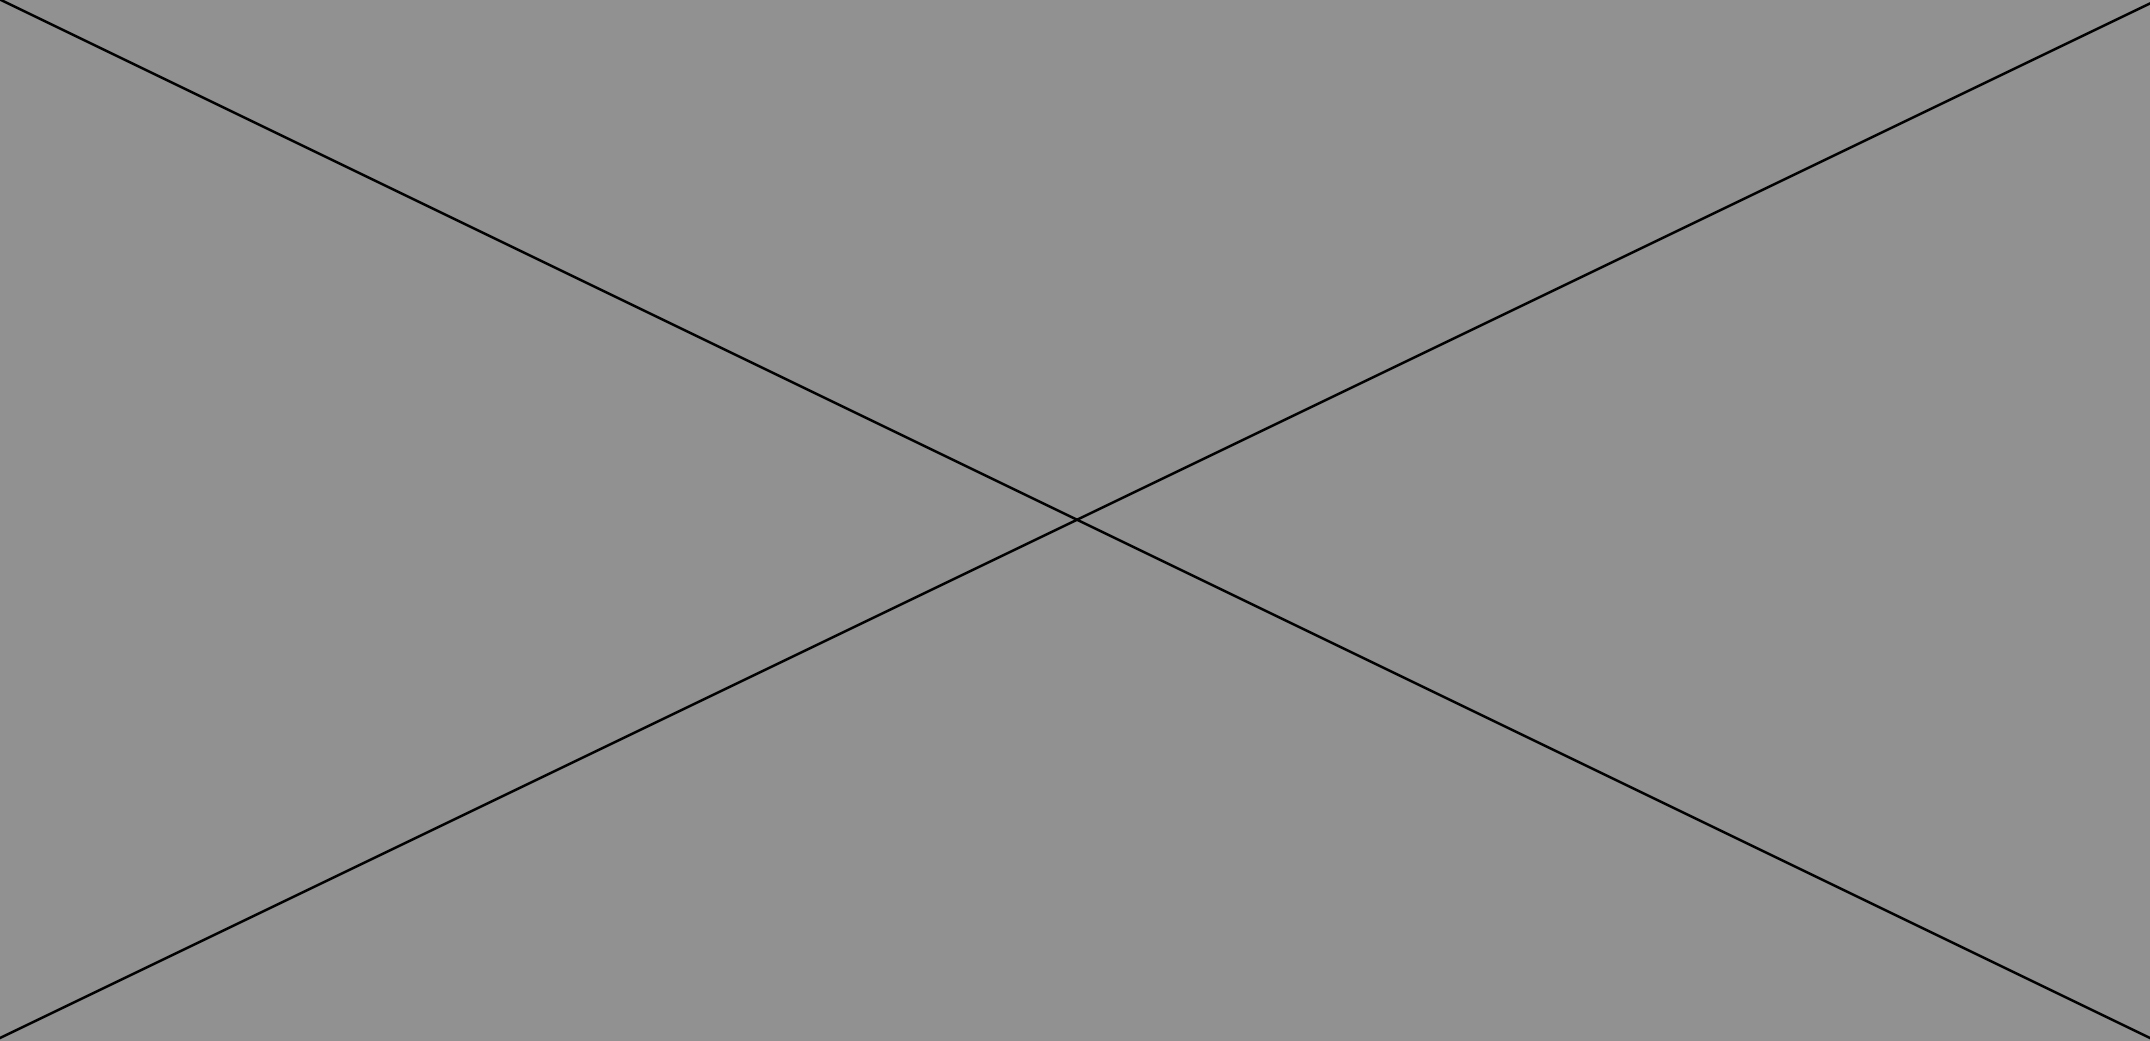
\includegraphics[width=.5\textwidth]{figures/placeholderImg.jpg}
  \caption[PT\_T1 Eye positioning]{PT\_T1 Eye positioning}
  \label{fig:PT_T1_pos}
\end{figure}

The sinusoidal tracking pattern (Fig.~\ref{fig:PT_T1_pos}) is evident from the plots of the y coordinate, while from the x coordinate plots it can be inferred that in the first half of the experiment the target moved from left to right (increase of x value) and then it travelled backwards (decrease of x value) following the same pattern (no disruption of the sinusoidal y pattern). The eye movements in the first 1000 ms are due to the focus-to-target routine in the stimuli. From the graph it can be seen that during two changes of directions (17.5 and 20 s) large saccades were performed, probably in the attempt to predict larger movements of the target. The left eye tracks smoothly the target sinusoidal movement with more precision, while the right eye is less precise. This is probably due to the dominance of the left eye over the right one in the subject.

\begin{figure}[h]
  \centering
  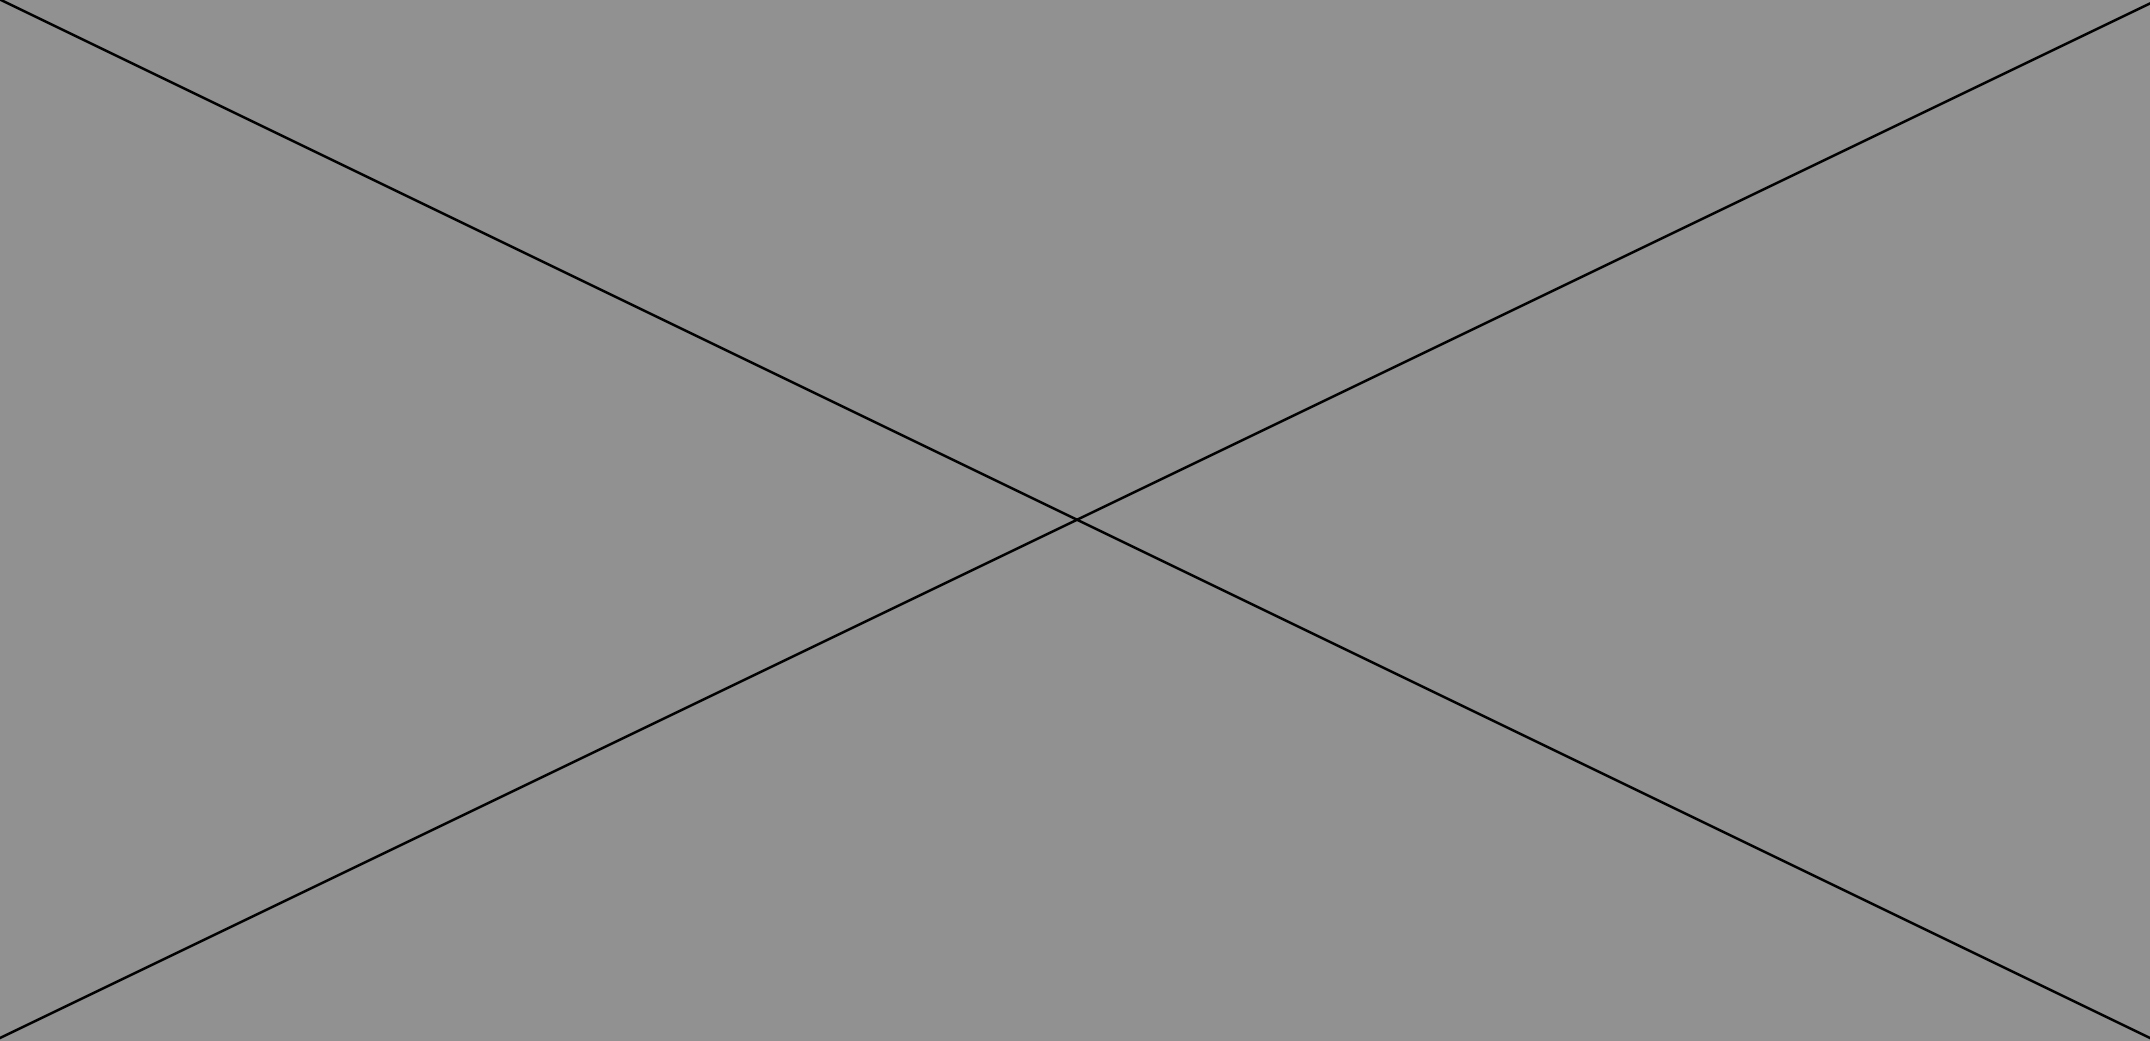
\includegraphics[width=.5\textwidth]{figures/placeholderImg.jpg}
  \caption[PT\_T1 pupil velocity]{PT\_T1 Pupil diameter and eye velocity}
  \label{fig:PT_T1_vel}
\end{figure}

Fig.~\ref{fig:PT_T1_vel} shows that a number of small saccades (the spikes in the eye velocity profile) were performed during the pursuit, and the two groups of larger saccades discussed in the chart Fig.~\ref{fig:PT_T1_pos} are well highlighted by high peaks of eye velocity.



\subsection{PT\_T2 : Triangular motion visual stimuli}
\label{sec:PT_T2}

\begin{figure}[h]
  \centering
  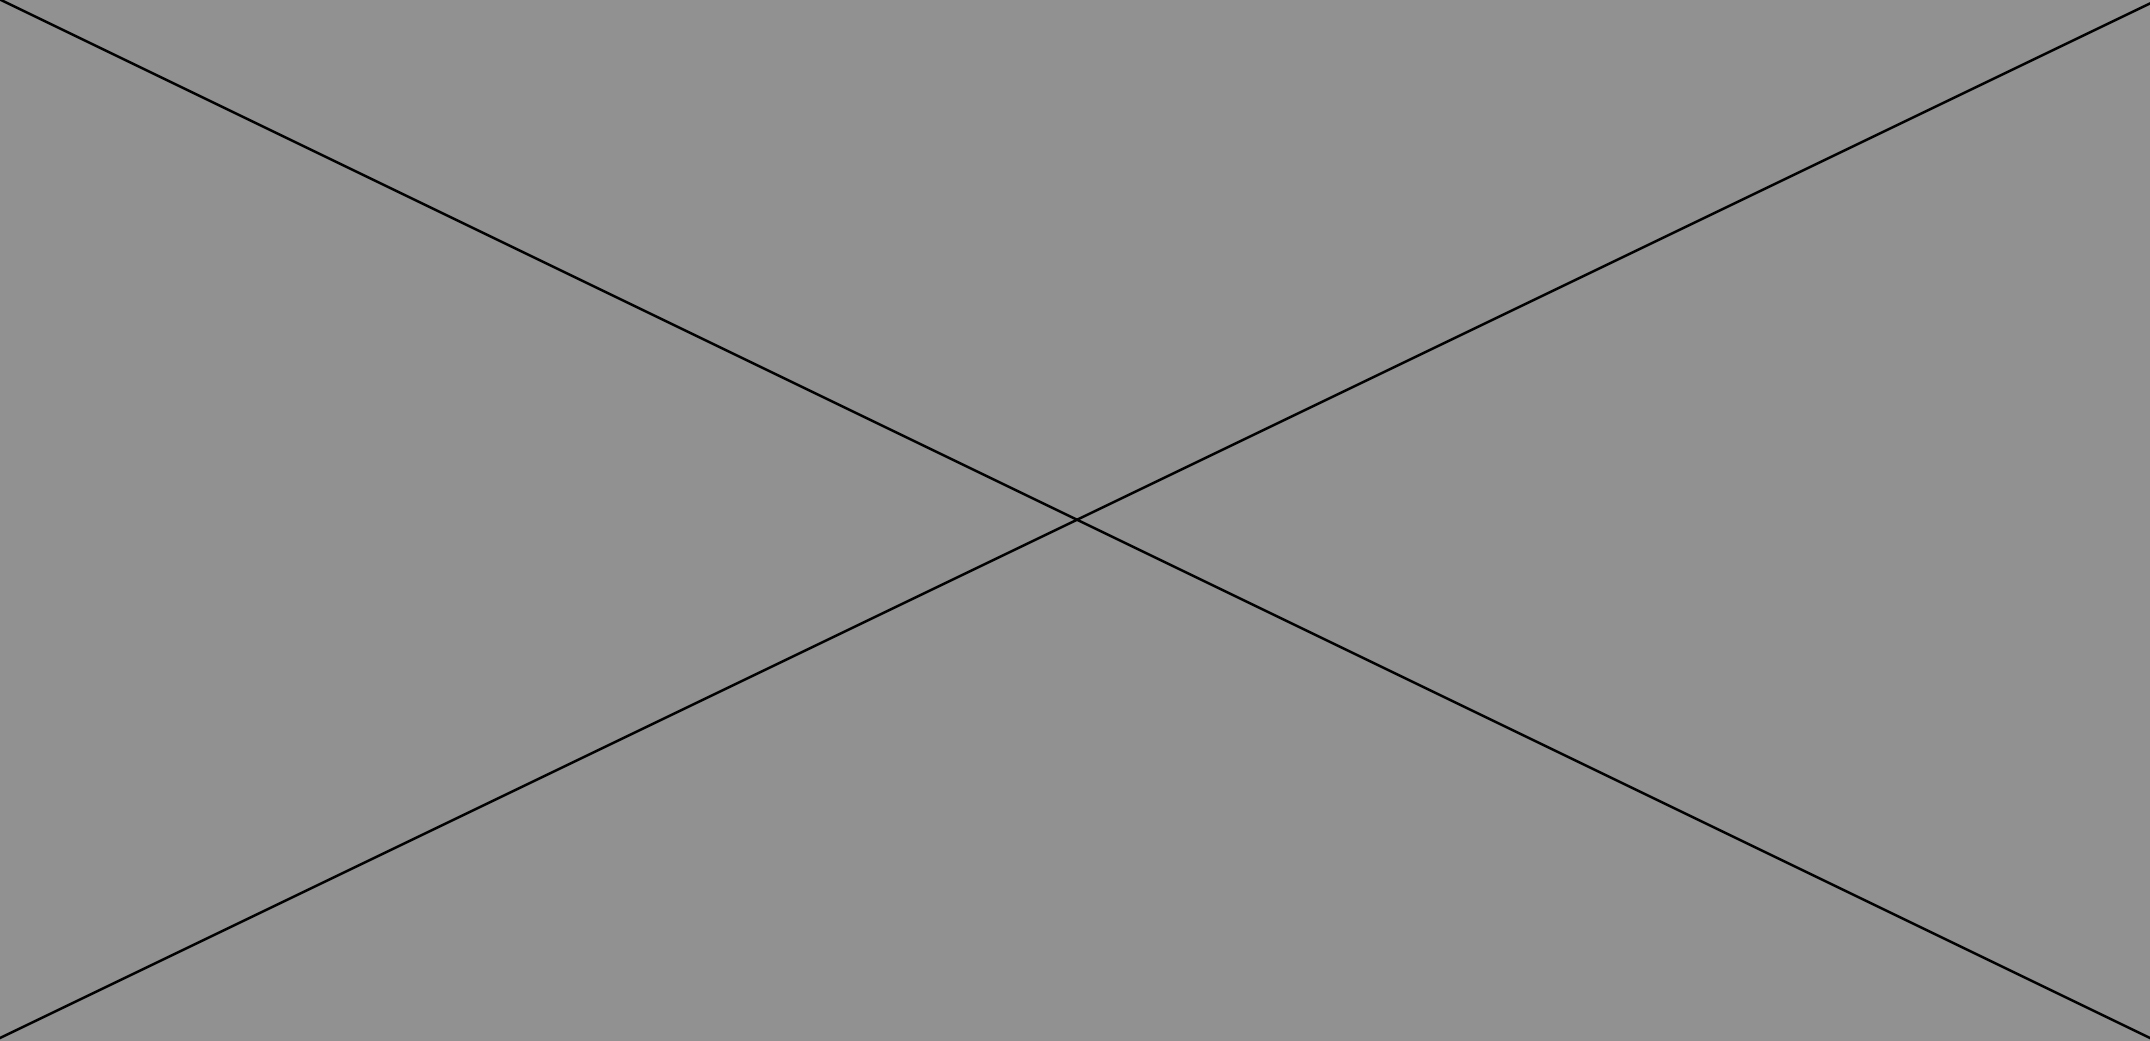
\includegraphics[width=.5\textwidth]{figures/placeholderImg.jpg}
  \caption[PT\_T2 Eye positioning]{PT\_T2 Eye positioning}
  \label{fig:PT_T2_pos}
\end{figure}

The considerations made for the sinusoidal motion chart (Fig.~\ref{fig:PT_T2_pos}) apply here to the triangular motion chart. Here it is even more evident the attempt to perform saccades at turning points of the target motion, which are indeed more abrupt than in the sinusoidal pattern.

\begin{figure}[h]
  \centering
  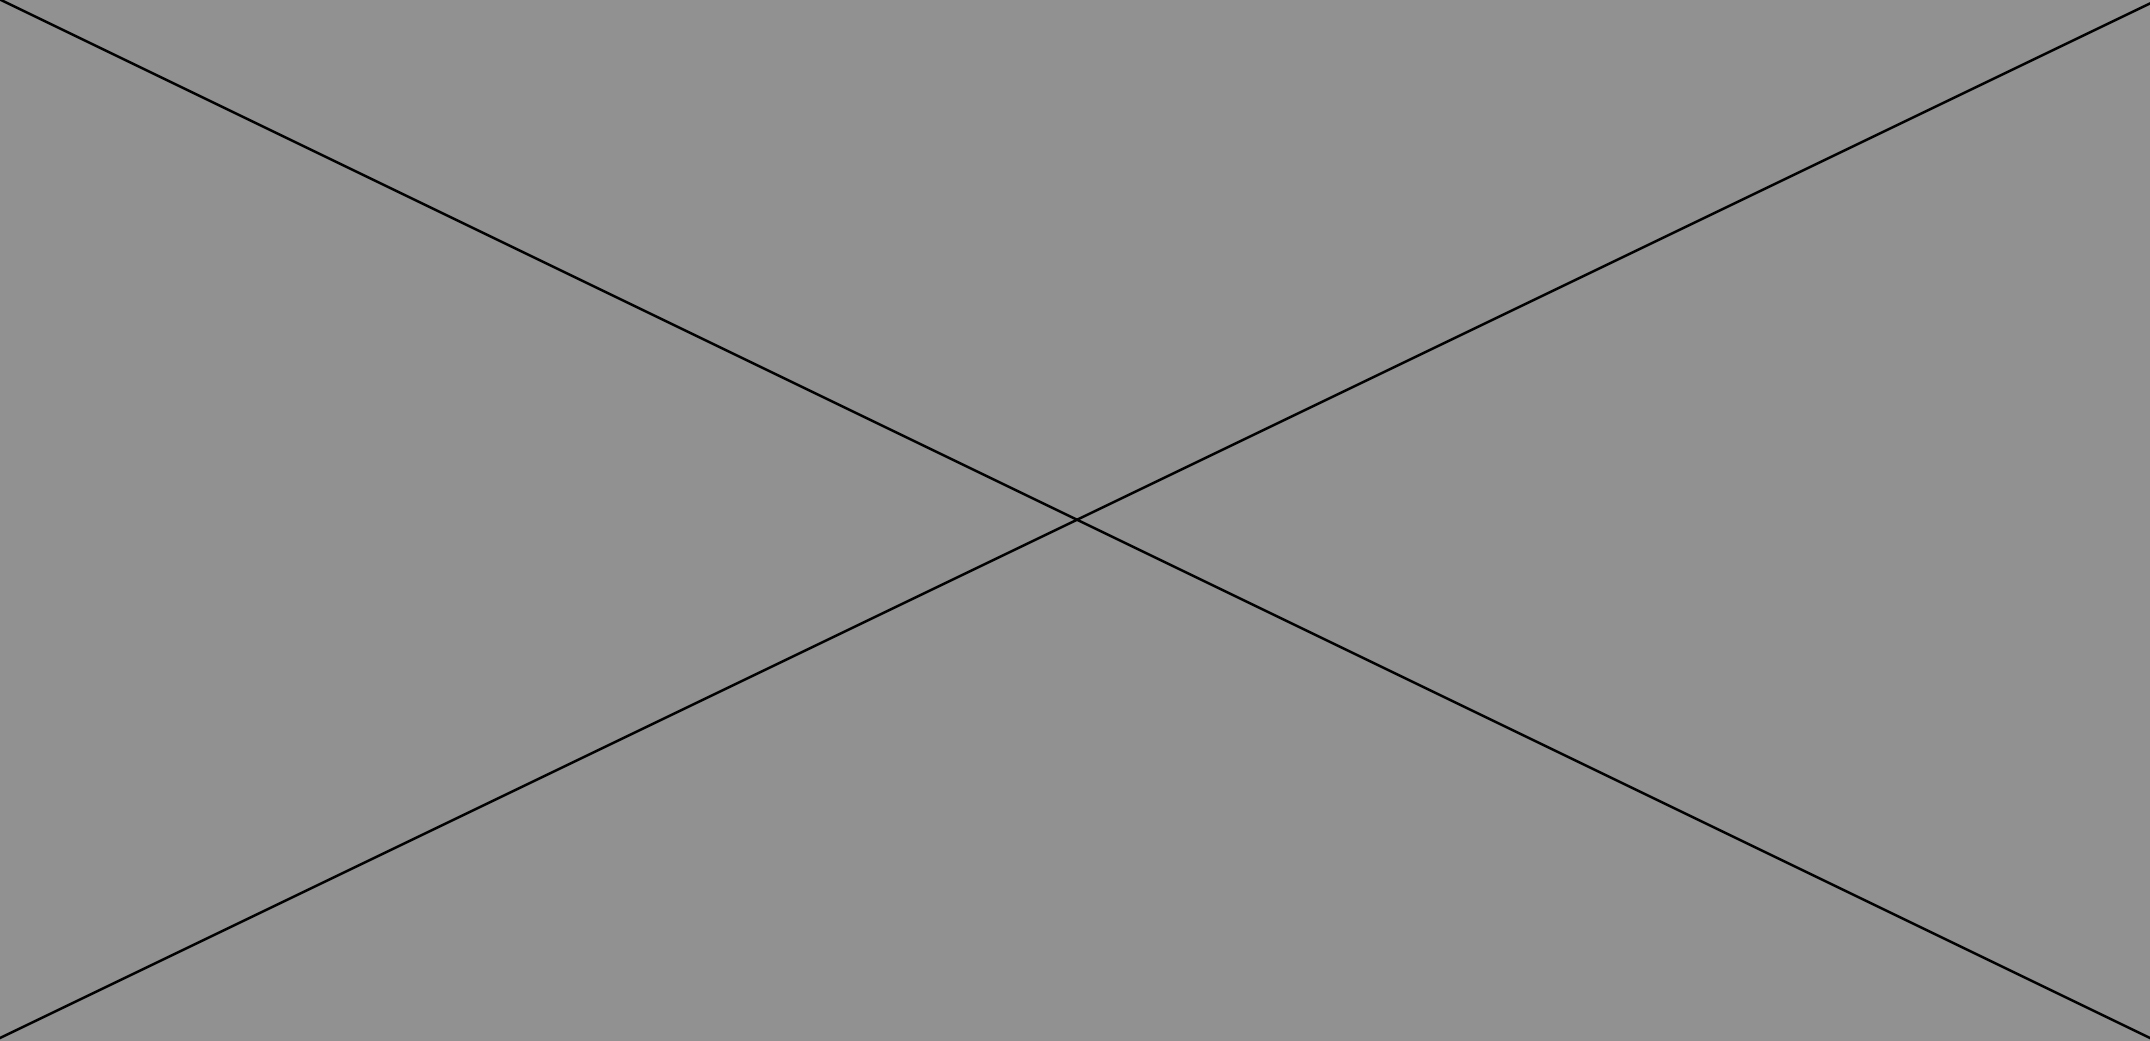
\includegraphics[width=.5\textwidth]{figures/placeholderImg.jpg}
  \caption[PT\_T2 Eye pupil velocity]{PT\_T2 Pupil diameter and eye velocity}
  \label{fig:PT_T2_vel}
\end{figure}

In Fig.~\ref{fig:PT_T2_vel}, it is possible to see that the during the smooth tracking the number of microsaccades appears to be lower than in the sinusoidal motion pattern. This is probably due to the fact that the triangular pattern has constant velocity, which should be easier for the oculomotor system to attune to. The three groups of large saccades are highlighted clearly by their peaks in velocity. The last peaks in velocity seem to be due more to a tracking loss.



\subsection{PT\_T3 : Step-Ramp pursuit visual stimuli}
\label{sec:PT_T3}

\begin{figure}[h]
  \centering
  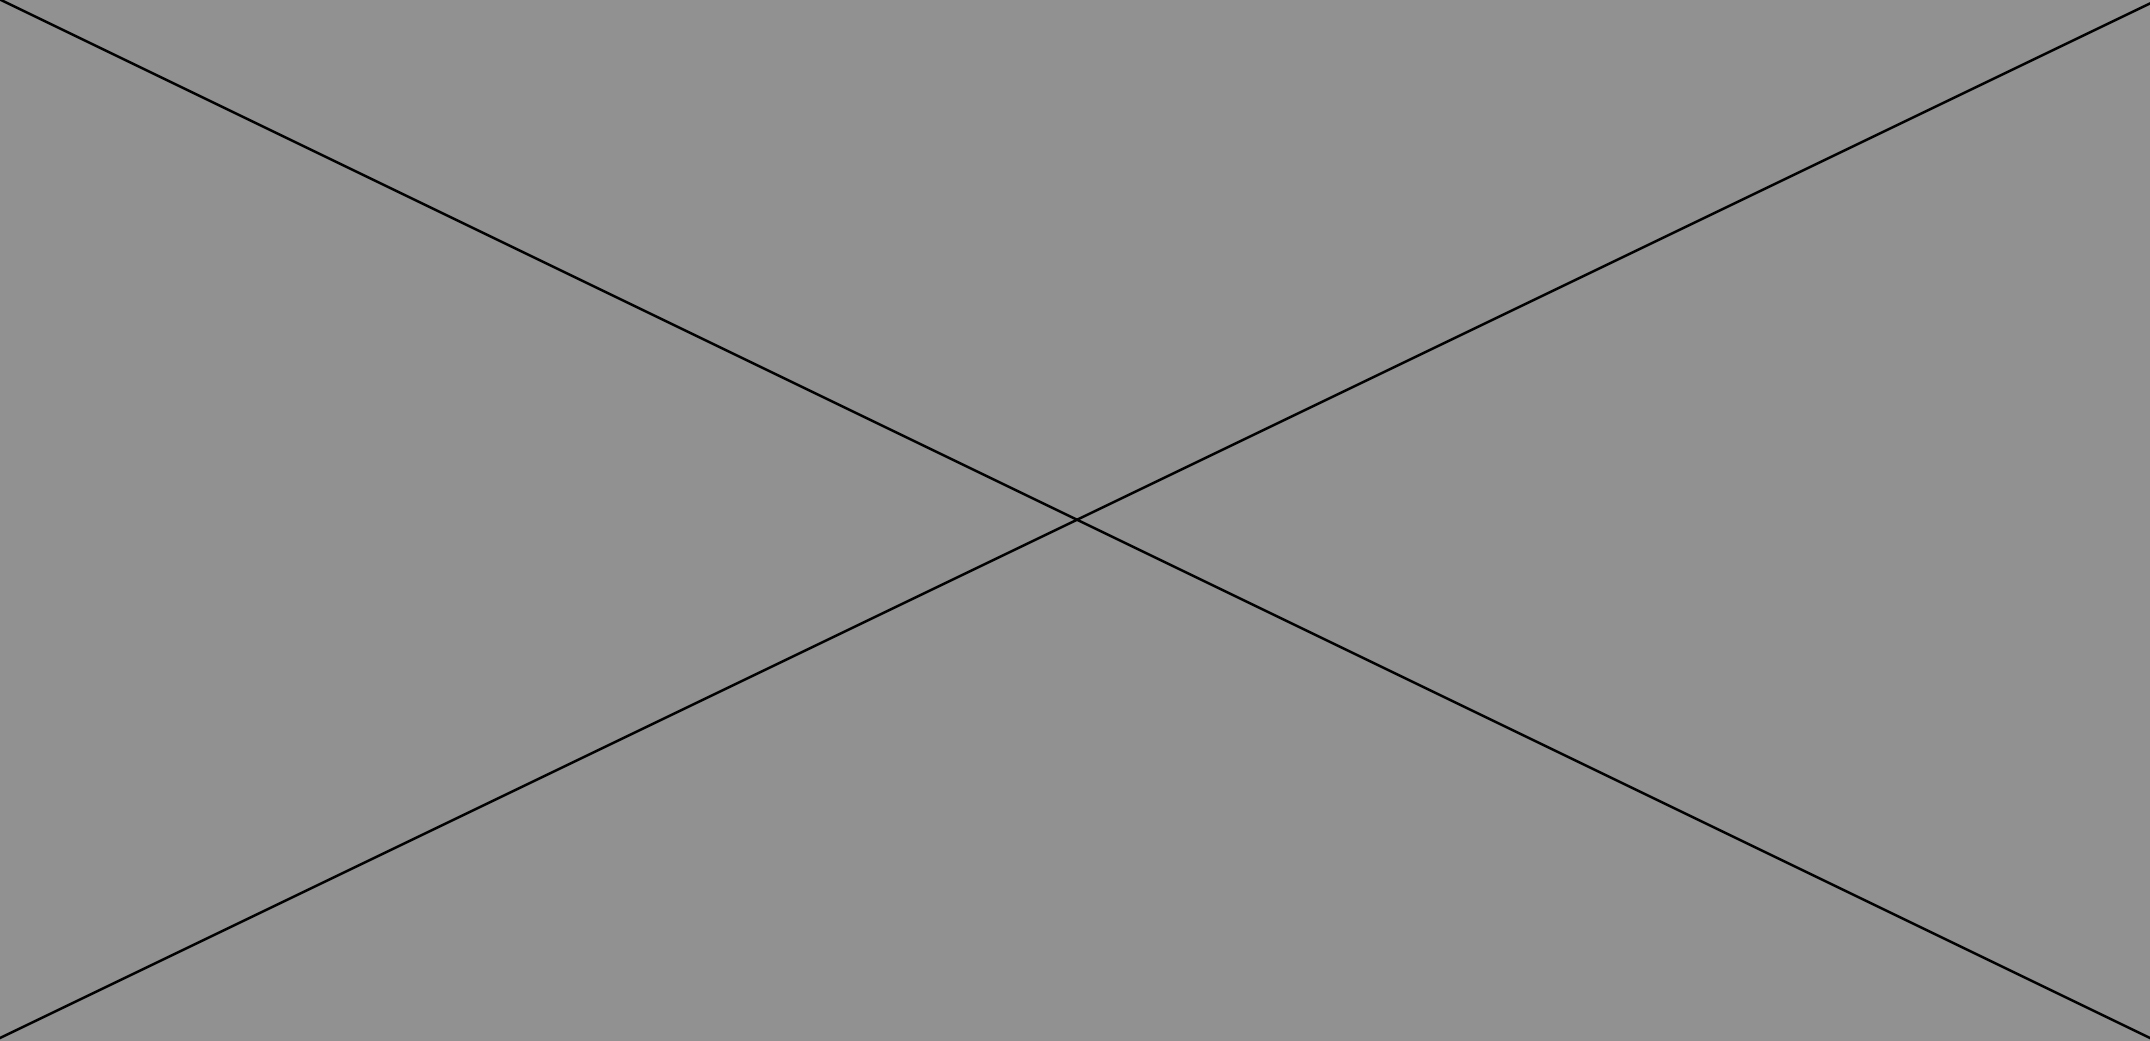
\includegraphics[width=.5\textwidth]{figures/placeholderImg.jpg}
  \caption[PT\_T3 Eye positioning]{PT\_T3 Eye positioning}
  \label{fig:PT_T3_pos}
\end{figure}

In Fig.~\ref{fig:PT_T3_pos} it is fairly clear to see the step-ramp paradigm in action. The x coordinate have a baseline of 960 px (since the target was displayed at the center of the screen, at half of the size of the stimuli, therefore 1920px/2). The eyes fixates at the baseline value, then they perform a rapid saccade towards the step location of 3 deg (positive or negative, either above or below the baseline), then they follow smoothly the target towards the final location of 15 deg (above or below the baseline depending on the direction) and finally they return to the baseline position at the start of the subsequent trial. The difference in time taken for completing the ramp pursuits is due to the different velocity profiles (4 or 8 deg/s).

The y coordinates of the eye movements are always equal, since the stimuli moves only on the horizontal axis. No large saccades or blinks are visible in the recorded data.

It is important to remind that even during fixations, a number of small eye movements are performed in order to prevent visual habituation \citep[p. 3]{leigh2015neurology}, therefore a completely flat velocity profile is not expected even during fixations.

\begin{figure}[h]
  \centering
  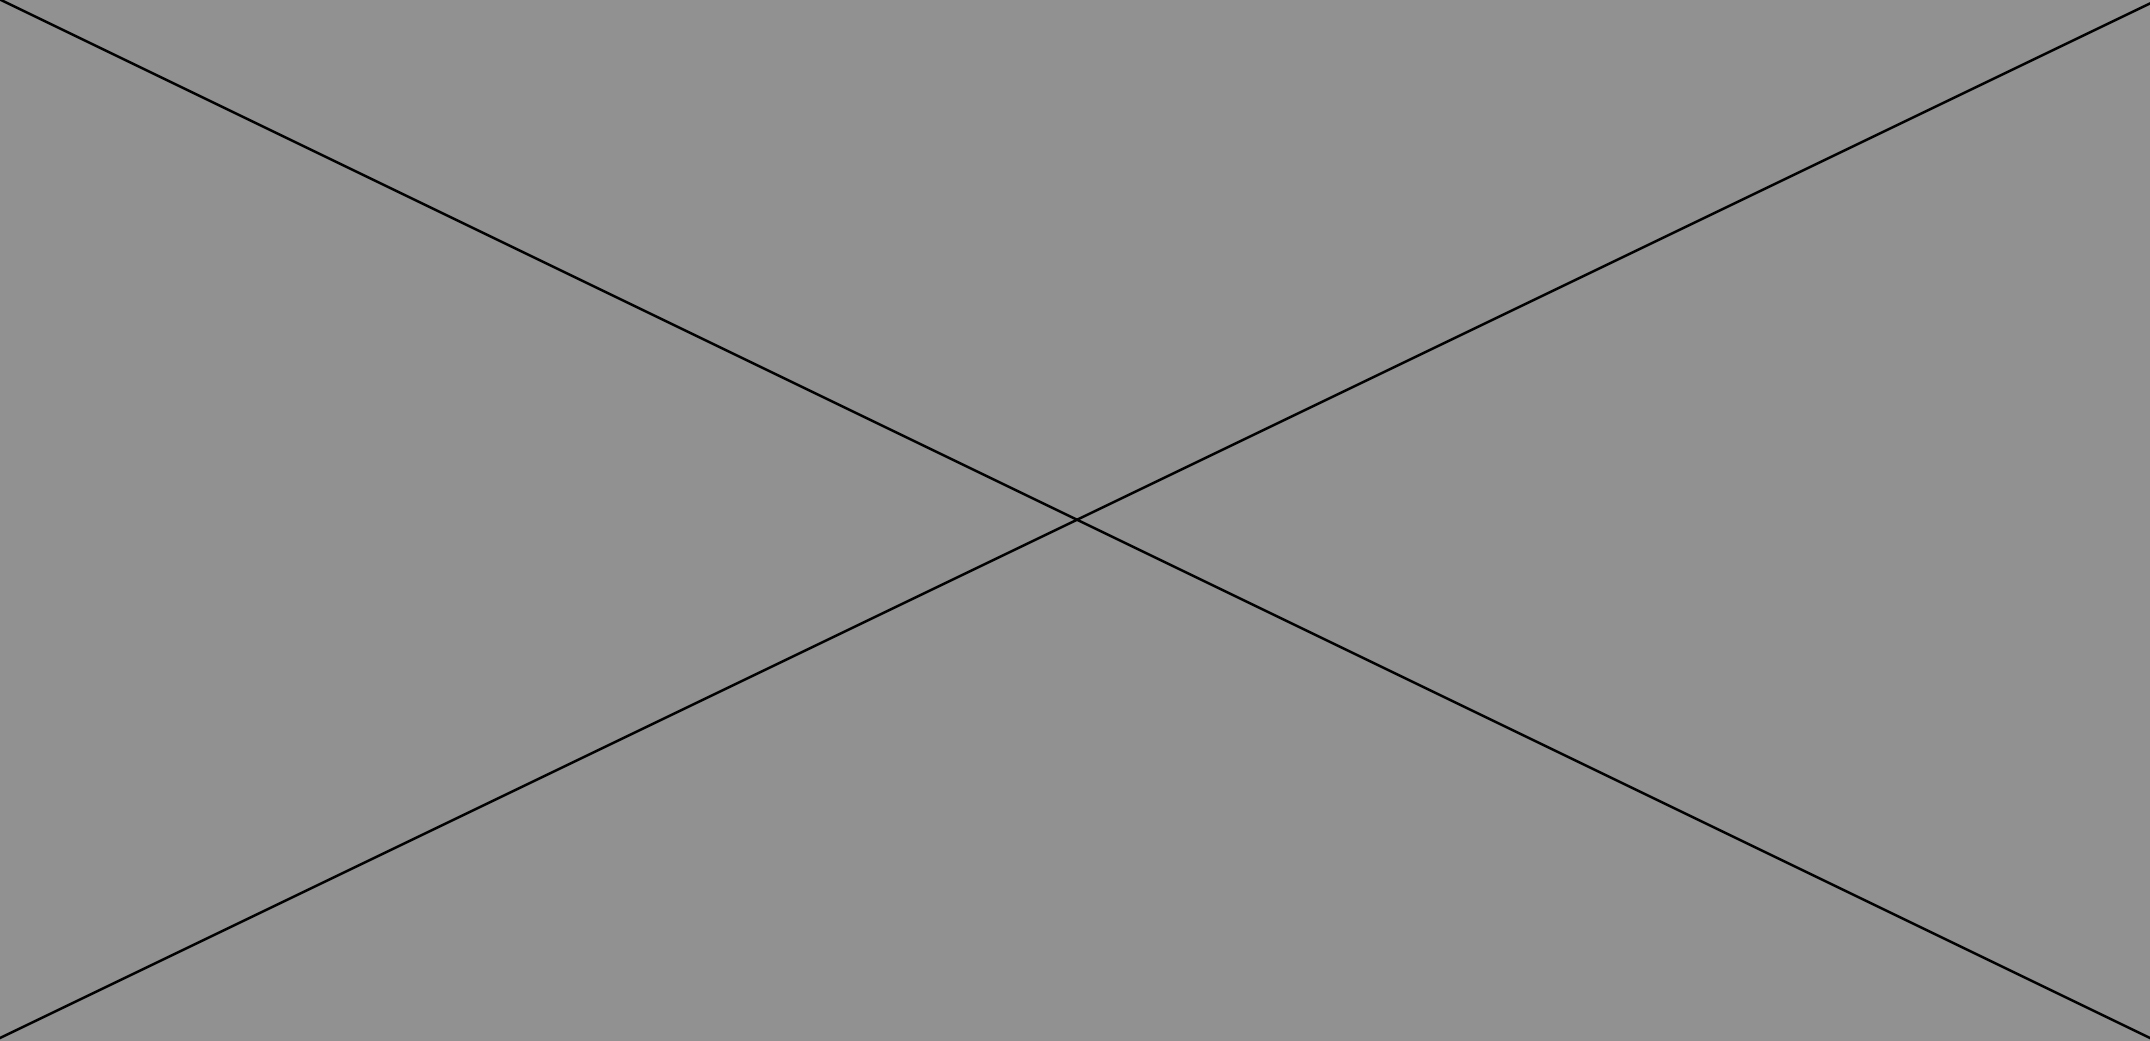
\includegraphics[width=.5\textwidth]{figures/placeholderImg.jpg}
  \caption[PT\_T3 pupil velocity]{PT\_T3 Pupil diameter and eye velocity}
  \label{fig:PT_T3_vel}
\end{figure}

In Fig.~\ref{fig:PT_T3_vel} it is possible to see the quick burst of more or less consistent velocity performed by the eyes in order to do the necessary saccade for the step. Then the smooth pursuit during the ramp flattens the velocity profile of the eye movements in a similar way than the fixations before the step do.


\subsection{PT\_T4 : Visually guided saccades visual stimuli}
\label{sec:PT_T4}

\begin{figure}[h]
  \centering
  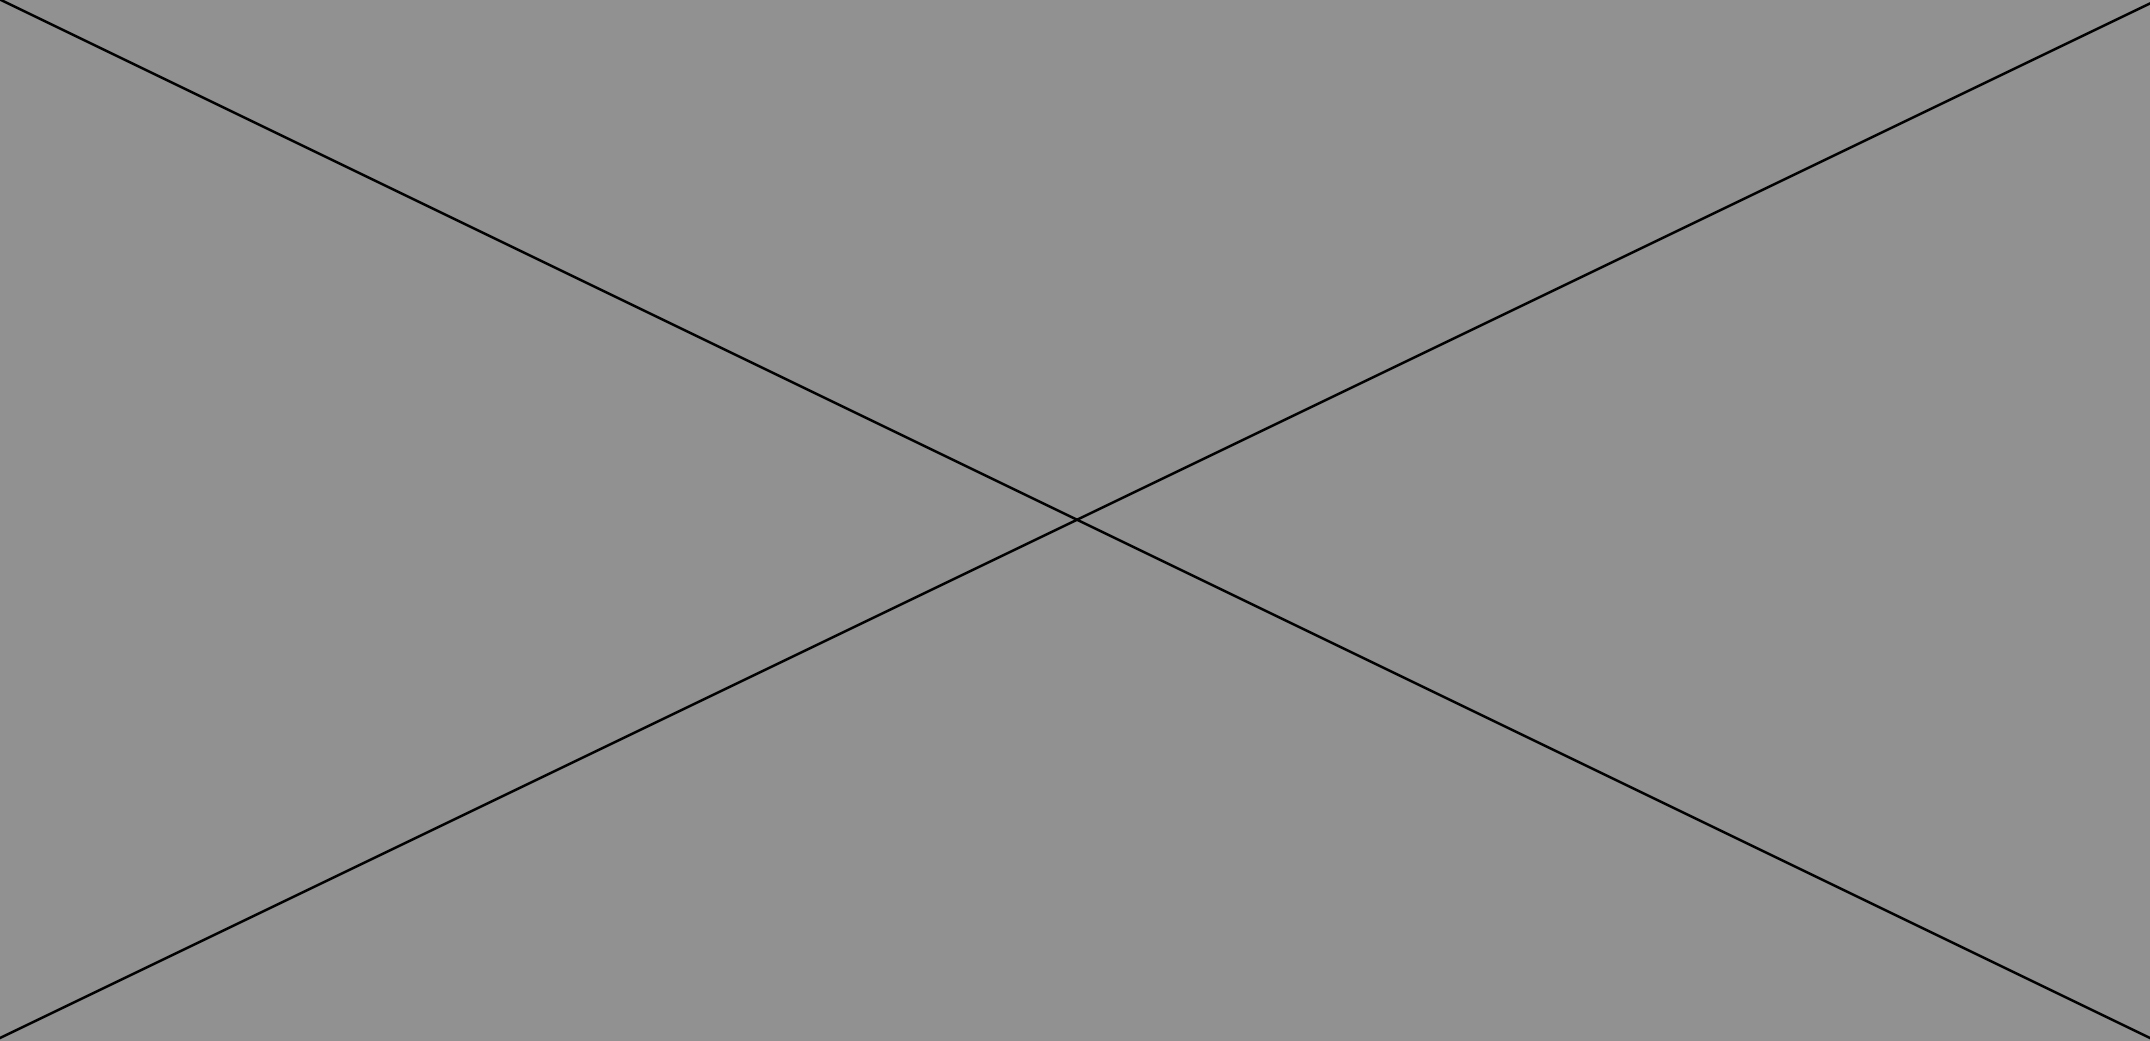
\includegraphics[width=.5\textwidth]{figures/placeholderImg.jpg}
  \caption[PT\_T4 Eye positioning]{PT\_T4 Eye positioning}
  \label{fig:PT_T4_pos}
\end{figure}

Fig.~\ref{fig:PT_T4_pos} shows how both the x and y coordinates of the eye change abruptly when a saccade is performed in order to track the target moving freely on the screen. The baseline value for the x value is 960 px while for the y value is 540 px (half of the stimulus size, since the target is at the center). The position profile moves upward or downward from the baseline basing on the direction of the target movement. Since the target stays both in the center and in the periphery for certain amounts of time, it is possible to see the fixation stabilization in between saccades. The trial lasted 43.7 s, but the chart focuses on the first 30 s in order to provide more details.

\begin{figure}[h]
  \centering
  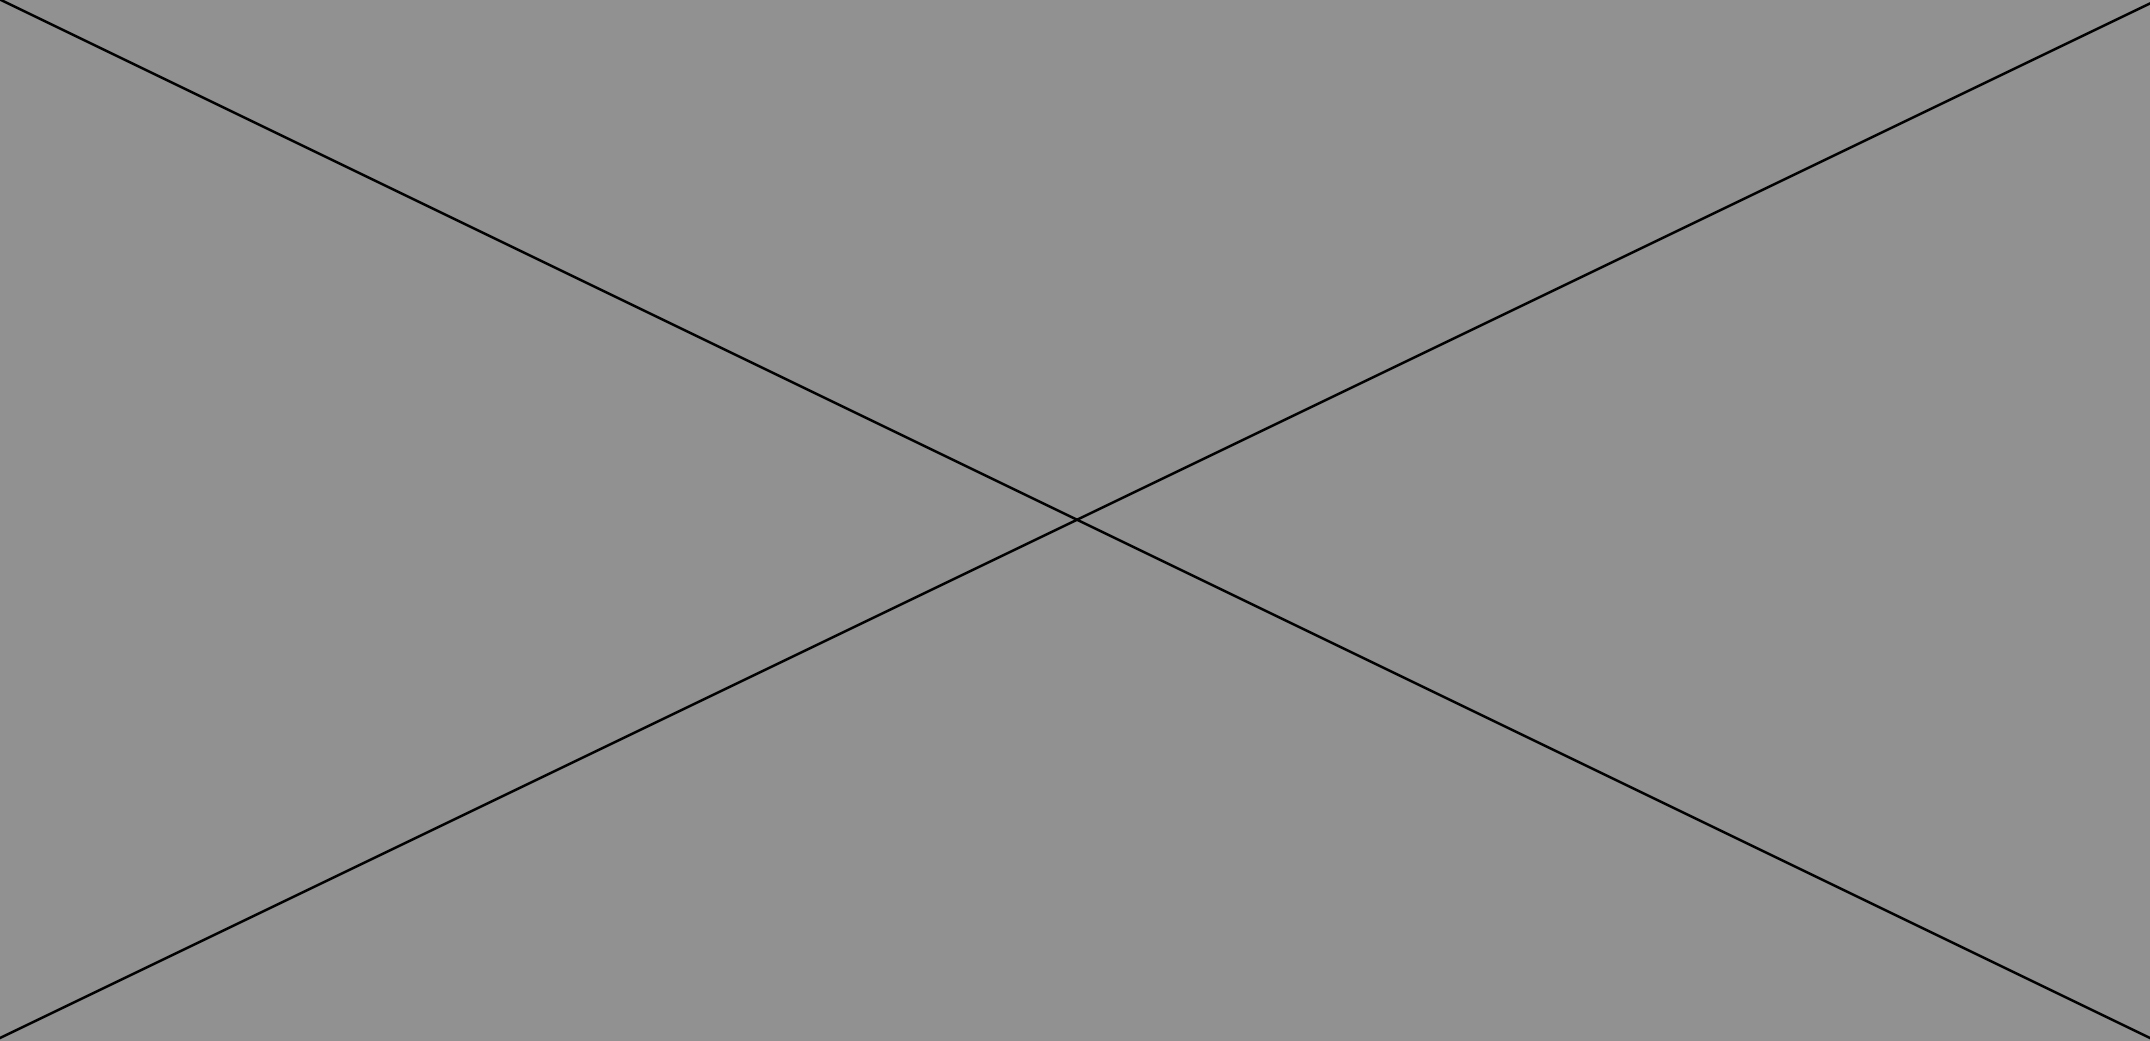
\includegraphics[width=.5\textwidth]{figures/placeholderImg.jpg}
  \caption[PT\_T4 pupil velocity]{PT\_T4 Pupil diameter and eye velocity}
  \label{fig:PT_T4_vel}
\end{figure}

Fig.~\ref{fig:PT_T4_vel} shows the bursts of eye velocity while performing the visually guided saccades, and the flat velocity profiles of the in-between fixations. It is interesting to notice that the first eye movement (performed between 1 and 2 seconds) has higher velocity and it is done in two saccades, therefore it was probably less precise. After that one, the other saccades are pretty similar, showing an attunement of the oculomotor system to the visual stimuli.





\section{Experimental group [P1, P2, P3]}
\label{sec:resexpgroup}

Tab.~\ref{tab:expgroupresultssummary} shows an overview of the results from the experiments with the target group (P1, P2 and P3).

\begin{table}[h]
  \centering
  \begin{tabular}{c|c}
    Age  & IQ  \\ 
    \hline
    10   & 100 \\
    20   & 100 \\
    30   & 150
  \end{tabular}
  \caption{P{1,2,3} experiments results overview}
  \label{tab:expgroupresultssummary}
\end{table}



\subsection{P{1,2,3}\_T1 : Sinusoidal motion visual stimuli}
\label{sec:P123_T1}

\subsubsection{P1\_T1}
\label{sec:P1_T1}

\begin{figure}[h]
  \centering
  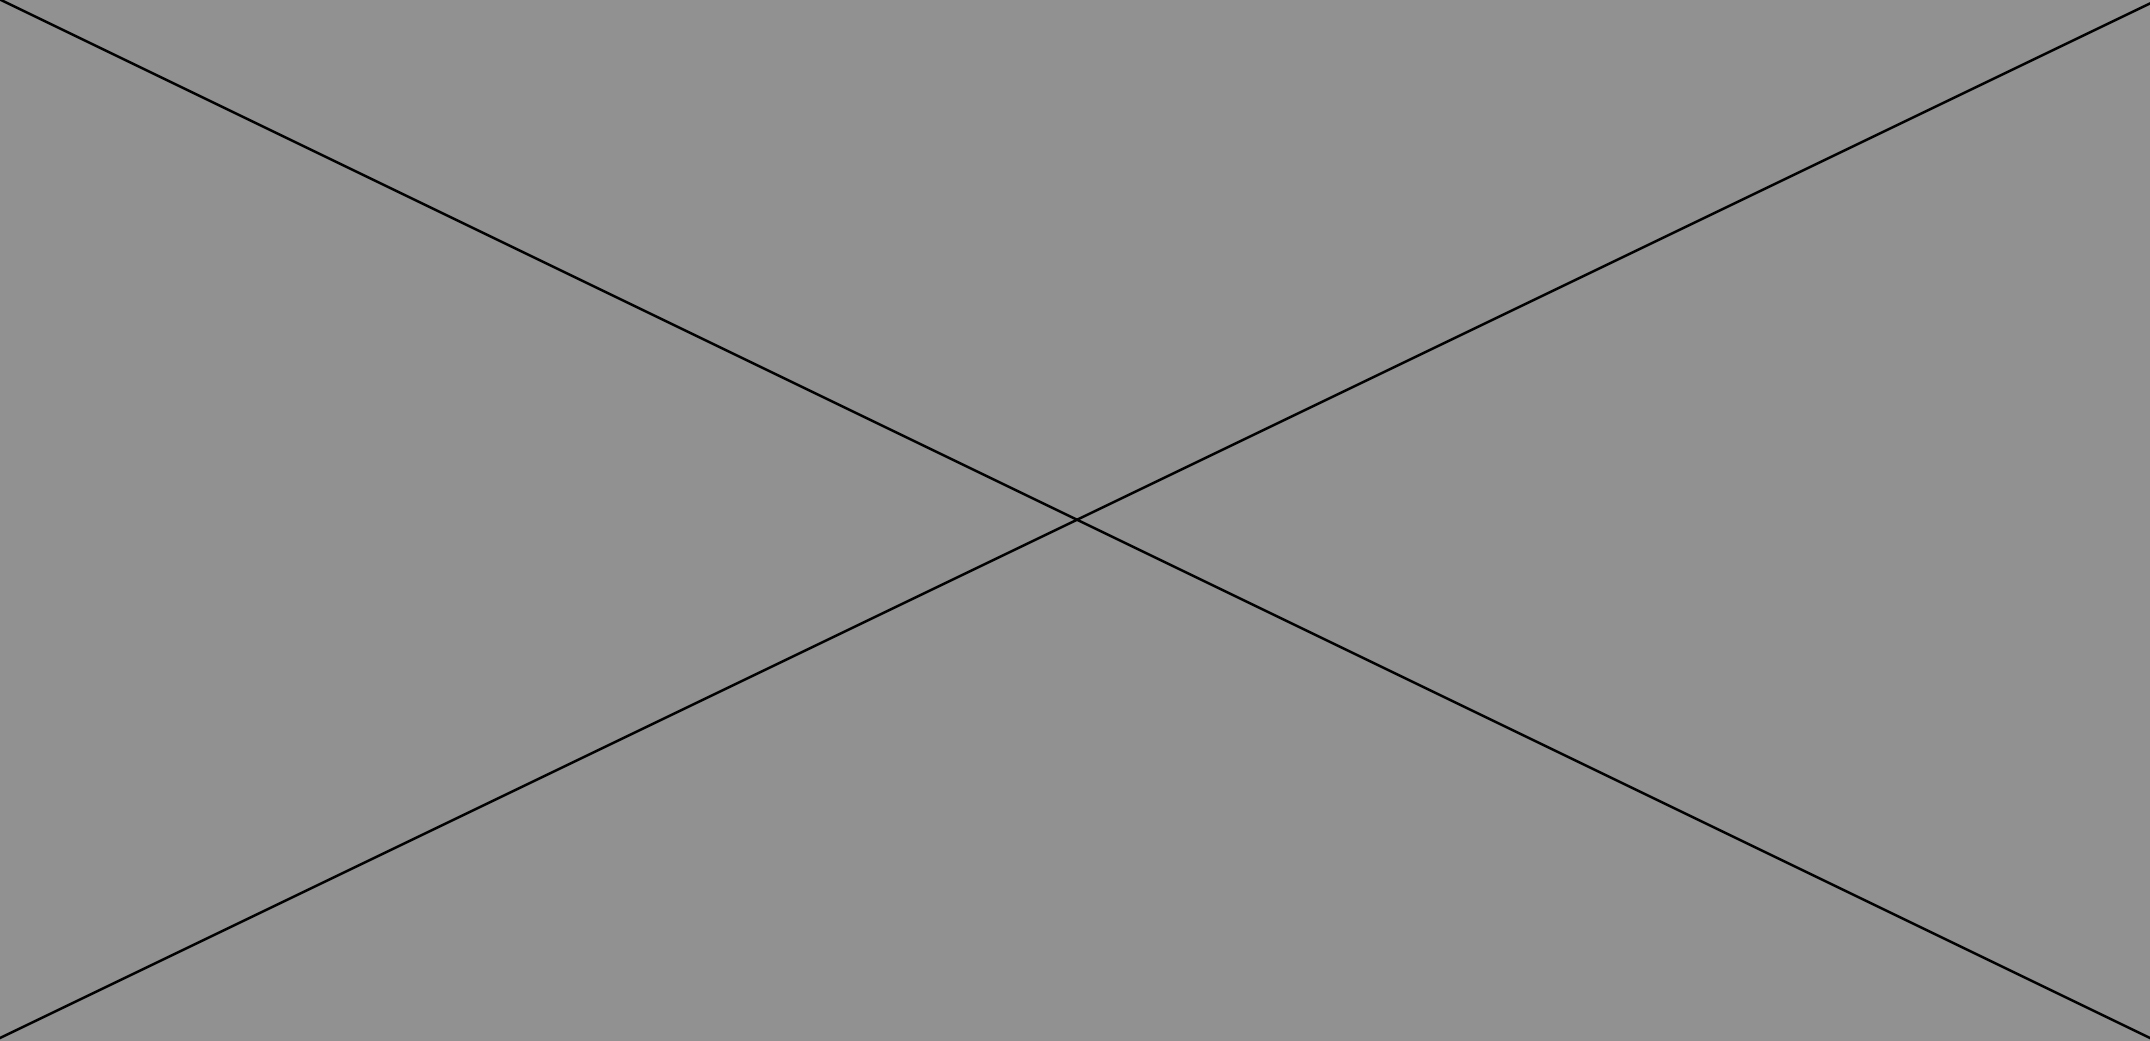
\includegraphics[width=.5\textwidth]{figures/placeholderImg.jpg}
  \caption[P1\_T1 Eye positioning]{P1\_T1 Eye positioning}
  \label{fig:P1_T1_pos}
\end{figure}

The visual stimuli elicited a gaze pattern (Fig.~\ref{fig:P1_T1_pos}) pretty close to the one expected for half of the designed repetitions. Indeed, the tracking record show data until the half of the experiment, while the target was moving in one direction from left to right. The graph show how P1’s eyes did not perform a very smooth pursuit especially near to the turning points and during the third repetition. Rather, it seems that they performed more of a series of saccades and fixations, drawing a “staircase” profile.
The graph also shows the intrusion of more or less large saccades especially immediately after the target turning points, which is consistent with the pilot test data.

\begin{figure}[h]
  \centering
  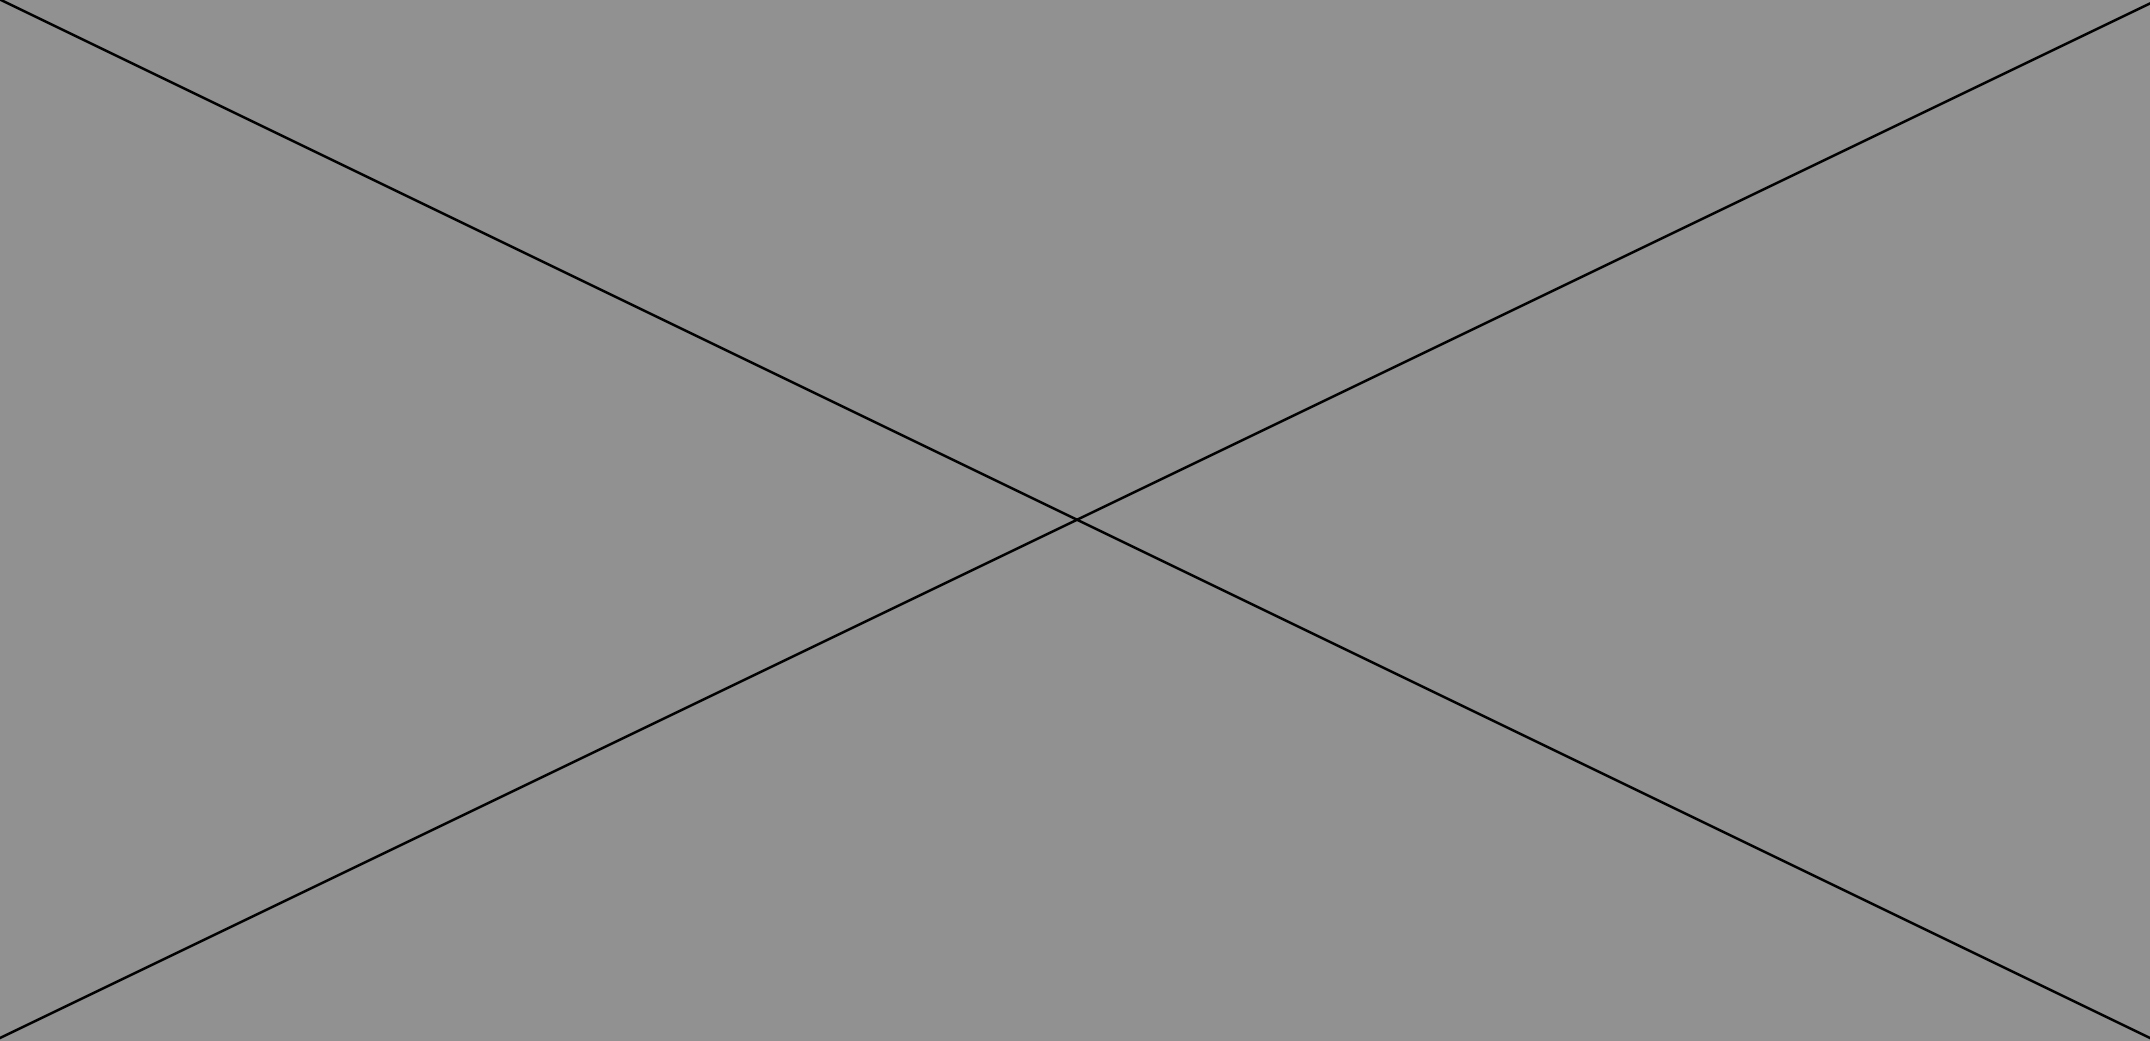
\includegraphics[width=.5\textwidth]{figures/placeholderImg.jpg}
  \caption[P1\_T1 pupil velocity]{P1\_T1 Pupil diameter and eye velocity}
  \label{fig:P1_T1_vel}
\end{figure}

Fig.~\ref{fig:P1_T1_vel} shows that during the smooth pursuit tracking in the first half of the stimuli presentation, P1 performed a series of small corrective saccades with small peaks of velocity, and also three large saccades with bursts of high peaks of velocity after the target turning points, where the eye velocity profile flattens the most since the target velocity is at minimum.


\subsubsection{P2\_T1}
\label{sec:P2_T1}

\begin{figure}[h]
  \centering
  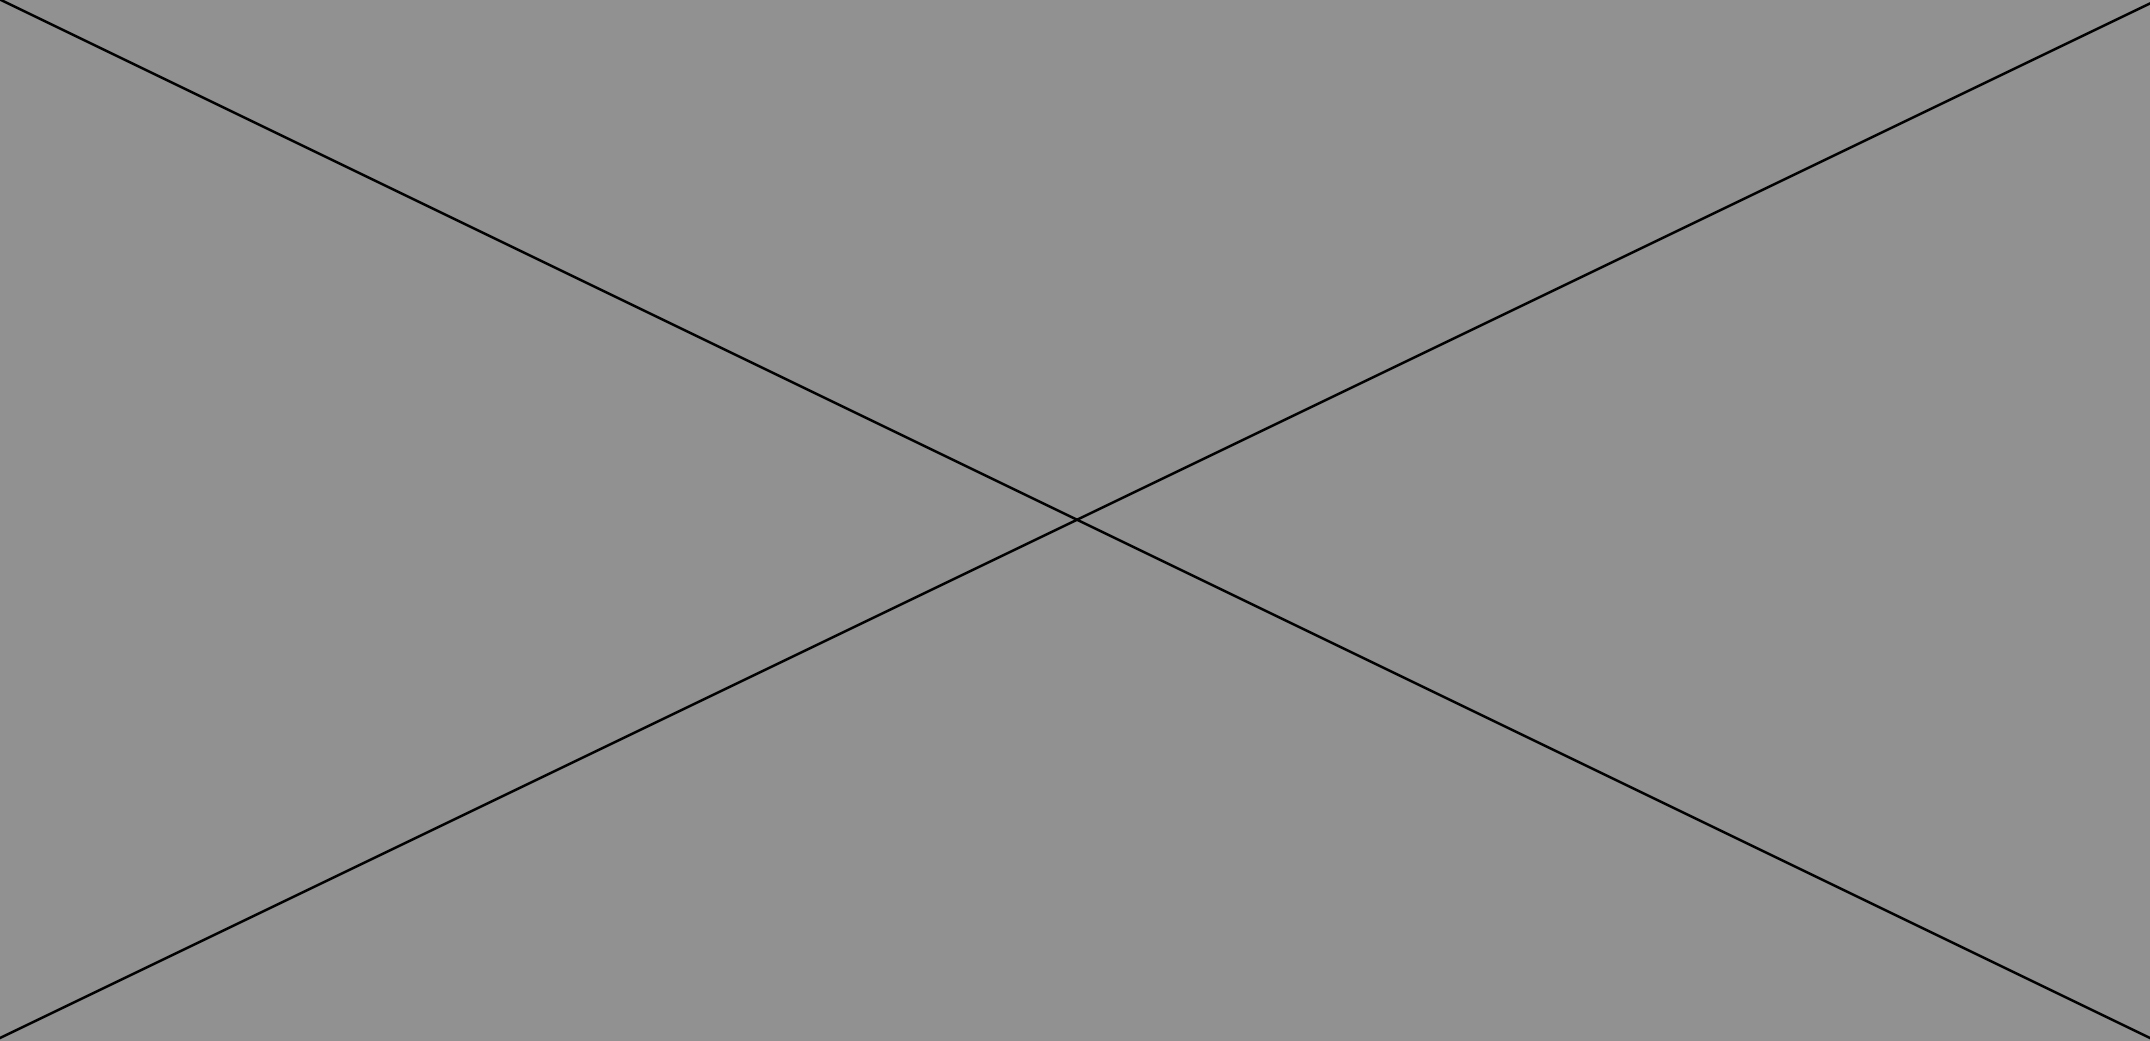
\includegraphics[width=.5\textwidth]{figures/placeholderImg.jpg}
  \caption[P2\_T1 Eye positioning]{P2\_T1 Eye positioning}
  \label{fig:P2_T1_pos}
\end{figure}

Fig.~\ref{fig:P1_T1_pos} shows that P2 tracked the sinusoidal moving target smoothly with noticeable accuracy throughout all the stimuli presentation. The eye tracker lost data on one full repetition and a half one, probably because the child moved a bit far away from the eye tracker or something caught her attention elsewhere. However, she returned to track the target again accurately. Two saccades, a small one and a large one, are visible before the target turning points, when the target starts decelerating noticeably.

\begin{figure}[h]
  \centering
  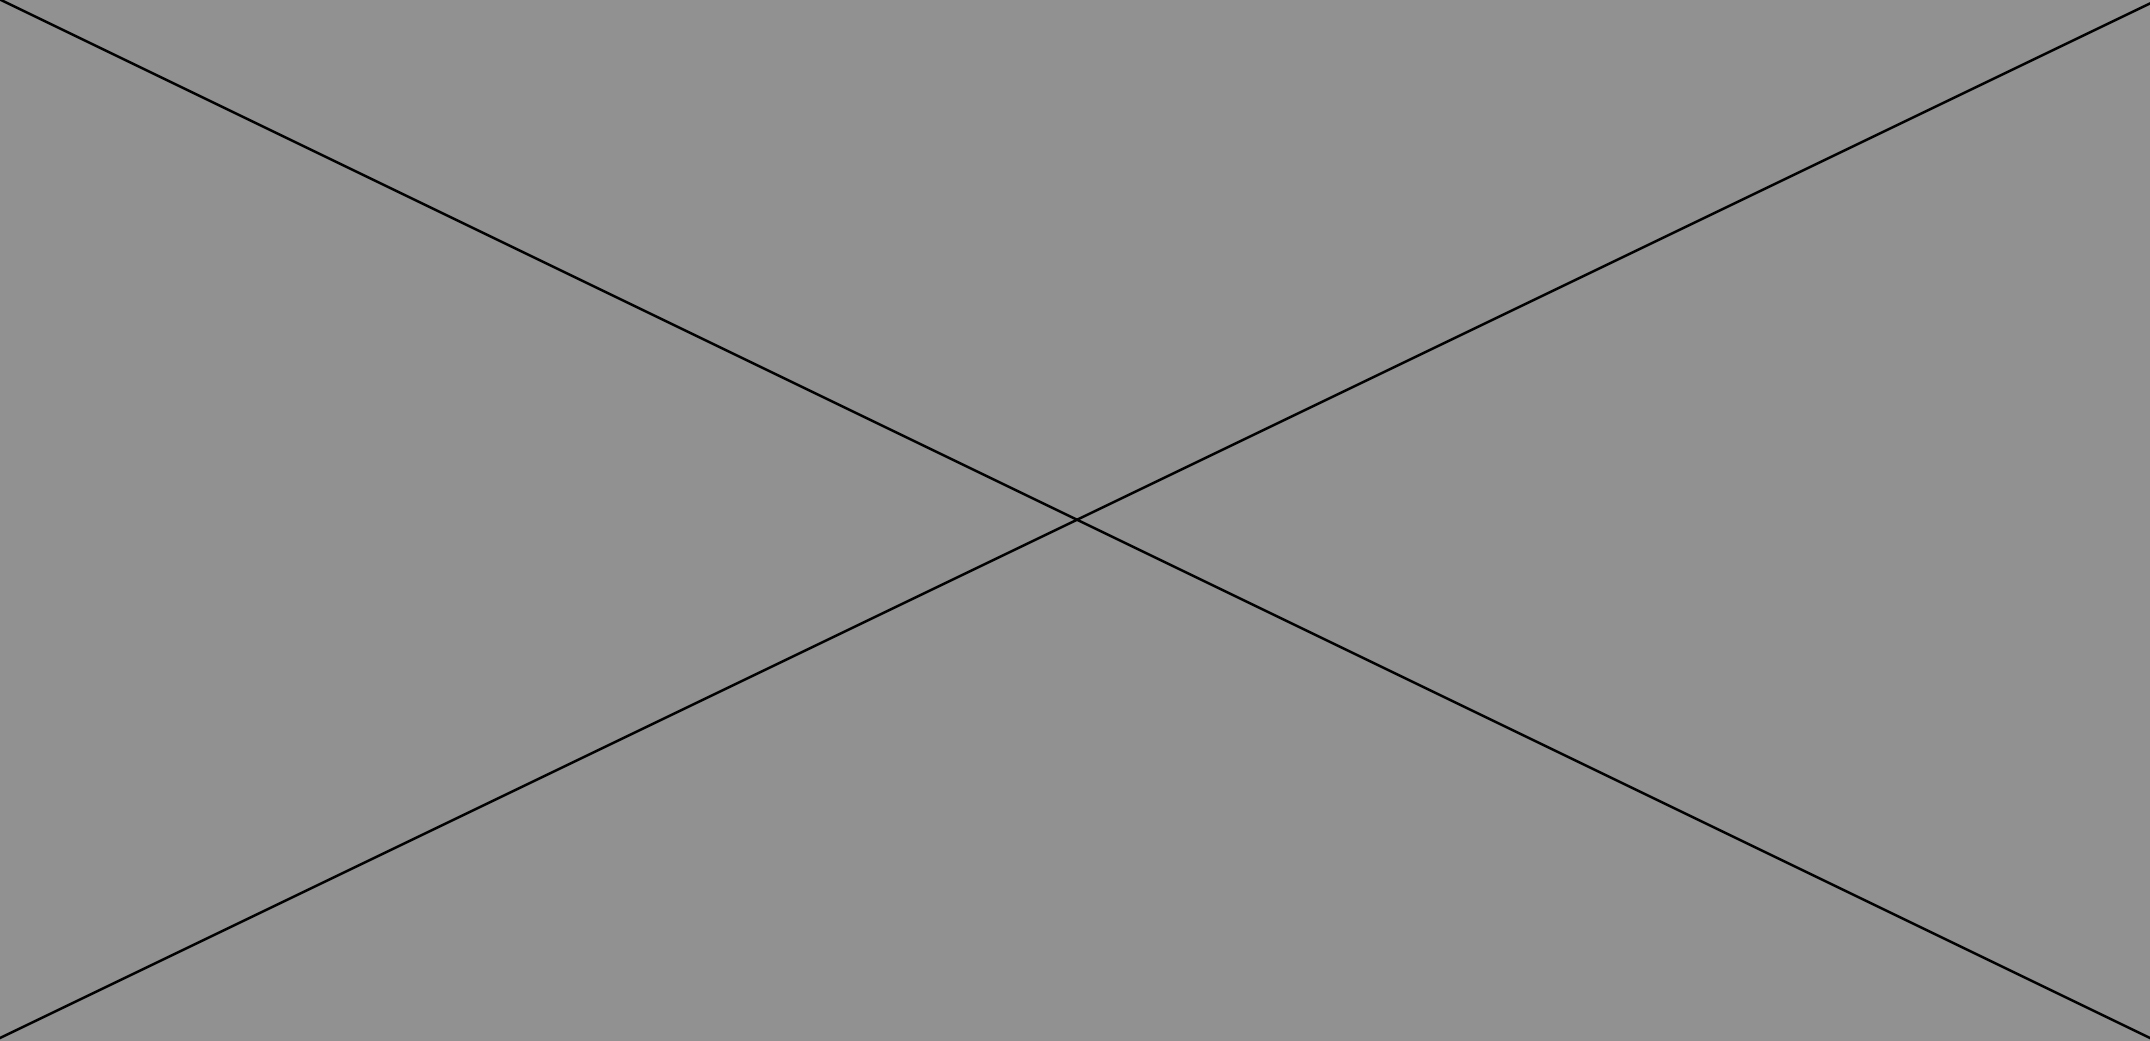
\includegraphics[width=.5\textwidth]{figures/placeholderImg.jpg}
  \caption[P2\_T1 pupil velocity]{P2\_T1 Pupil diameter and eye velocity}
  \label{fig:P2_T1_vel}
\end{figure}

Fig.~\ref{fig:P2_T1_vel} show how during smooth tracking the velocity profile of P2 eyes is near to be flat, meaning that even though the eyes were moving constantly, P2 made no saccades or abrupt eye movements. Bursts of high peaks of eye velocity are found during larger saccades intrusions.



\subsubsection{P3\_T1}
\label{sec:P3_T1}

\begin{figure}[h]
  \centering
  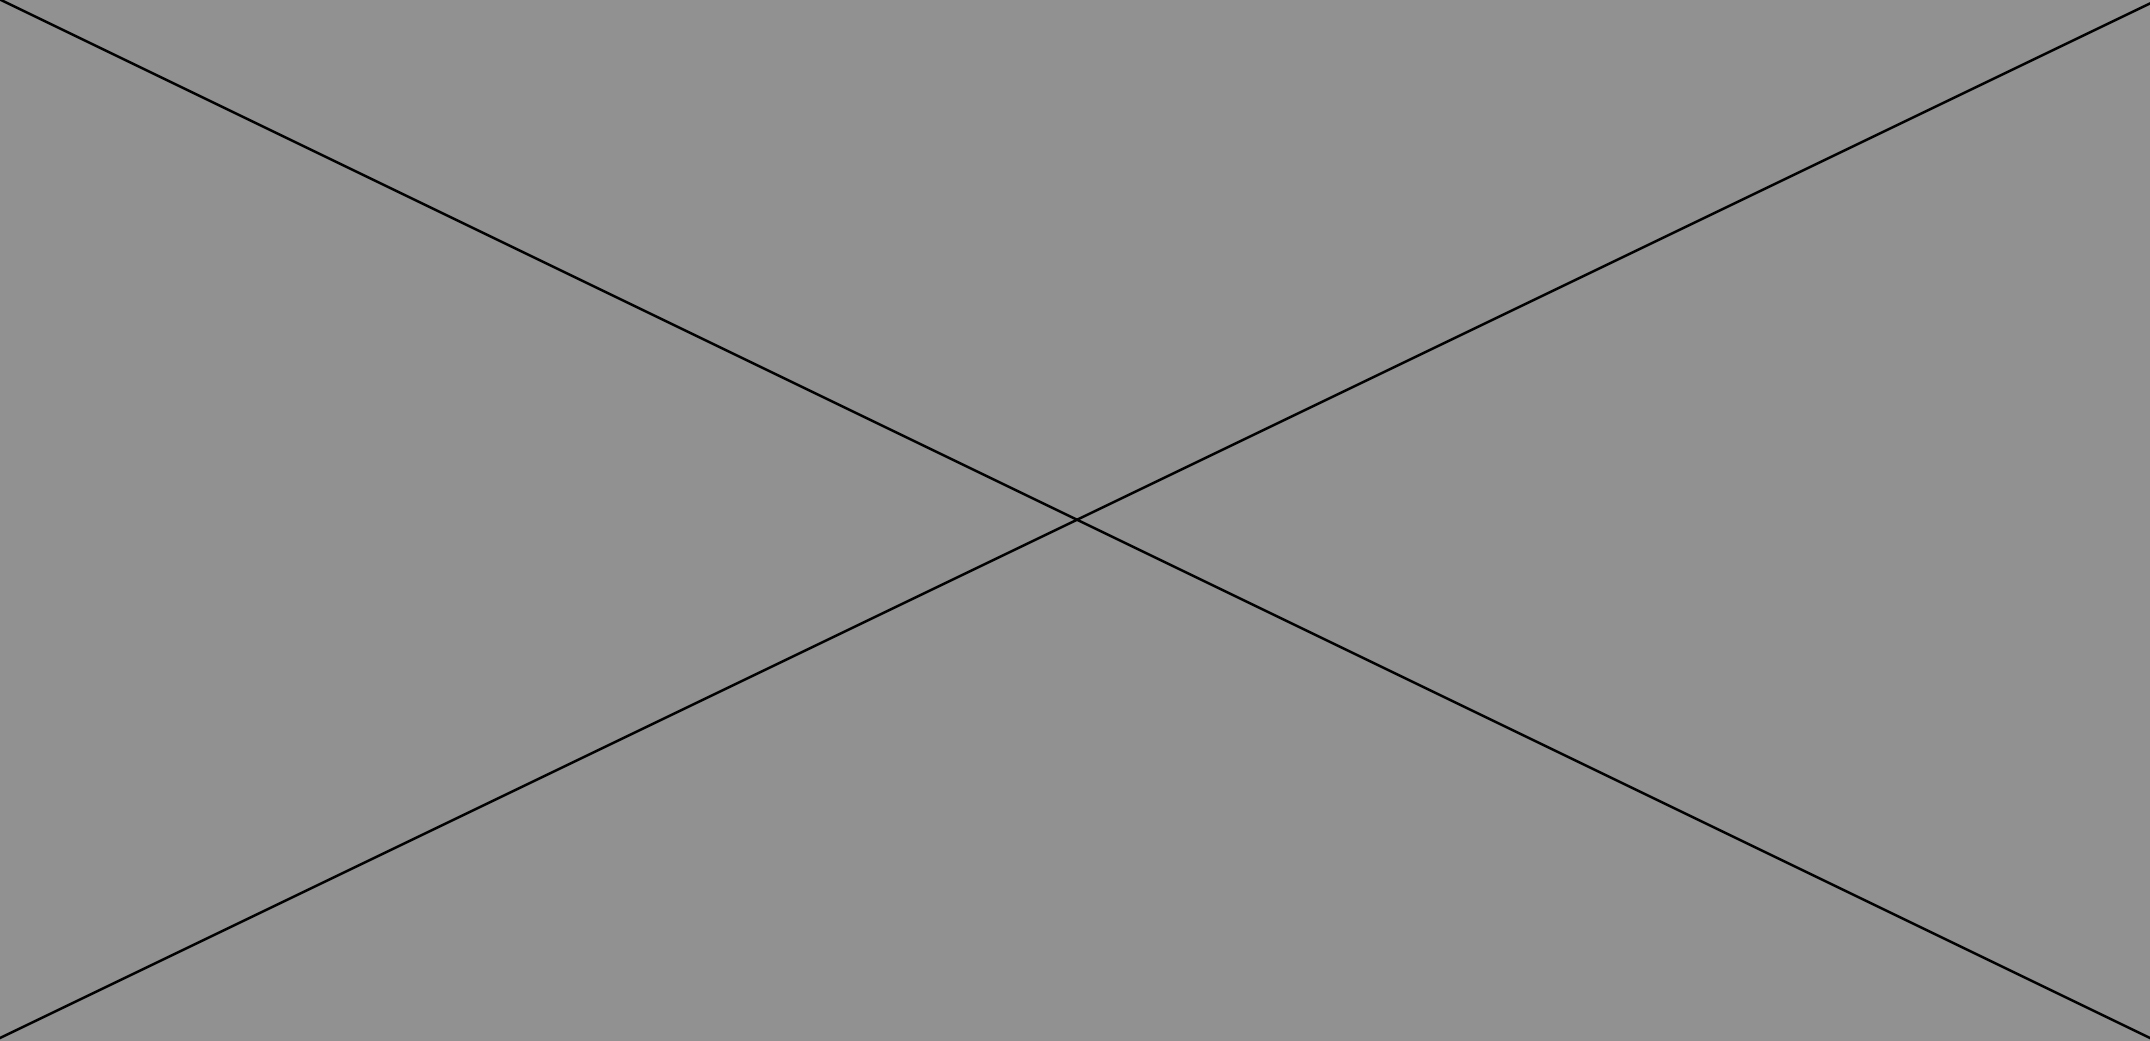
\includegraphics[width=.5\textwidth]{figures/placeholderImg.jpg}
  \caption[P3\_T1 Eye positioning]{P3\_T1 Eye positioning}
  \label{fig:P3_T1_pos}
\end{figure}

As Fig.~\ref{fig:P3_T1_pos} shows, the quantity of collected data from P3 in the first trial is rather low (tracking ratio 23,6\%). This is probably due to the fact that the child might become comfortable to sit in a position too far away from the display monitor. Or it can be due to the fact that the child seemed very curious towards the researchers and was more keen on observing them than the display monitor. These events are expected to happen while testing with such a small baby. Therefore, it is not possible to state that the recorded data can be useful for an in-deep analysis. However, in the only full repetition completely recorded as well as in the first section of another one, it is possible to see that the stimuli elicited the expected sinusoidal gaze pattern. Moreover, the smooth tracking shows qualitatively the same staircase profile of P1.

\begin{figure}[h]
  \centering
  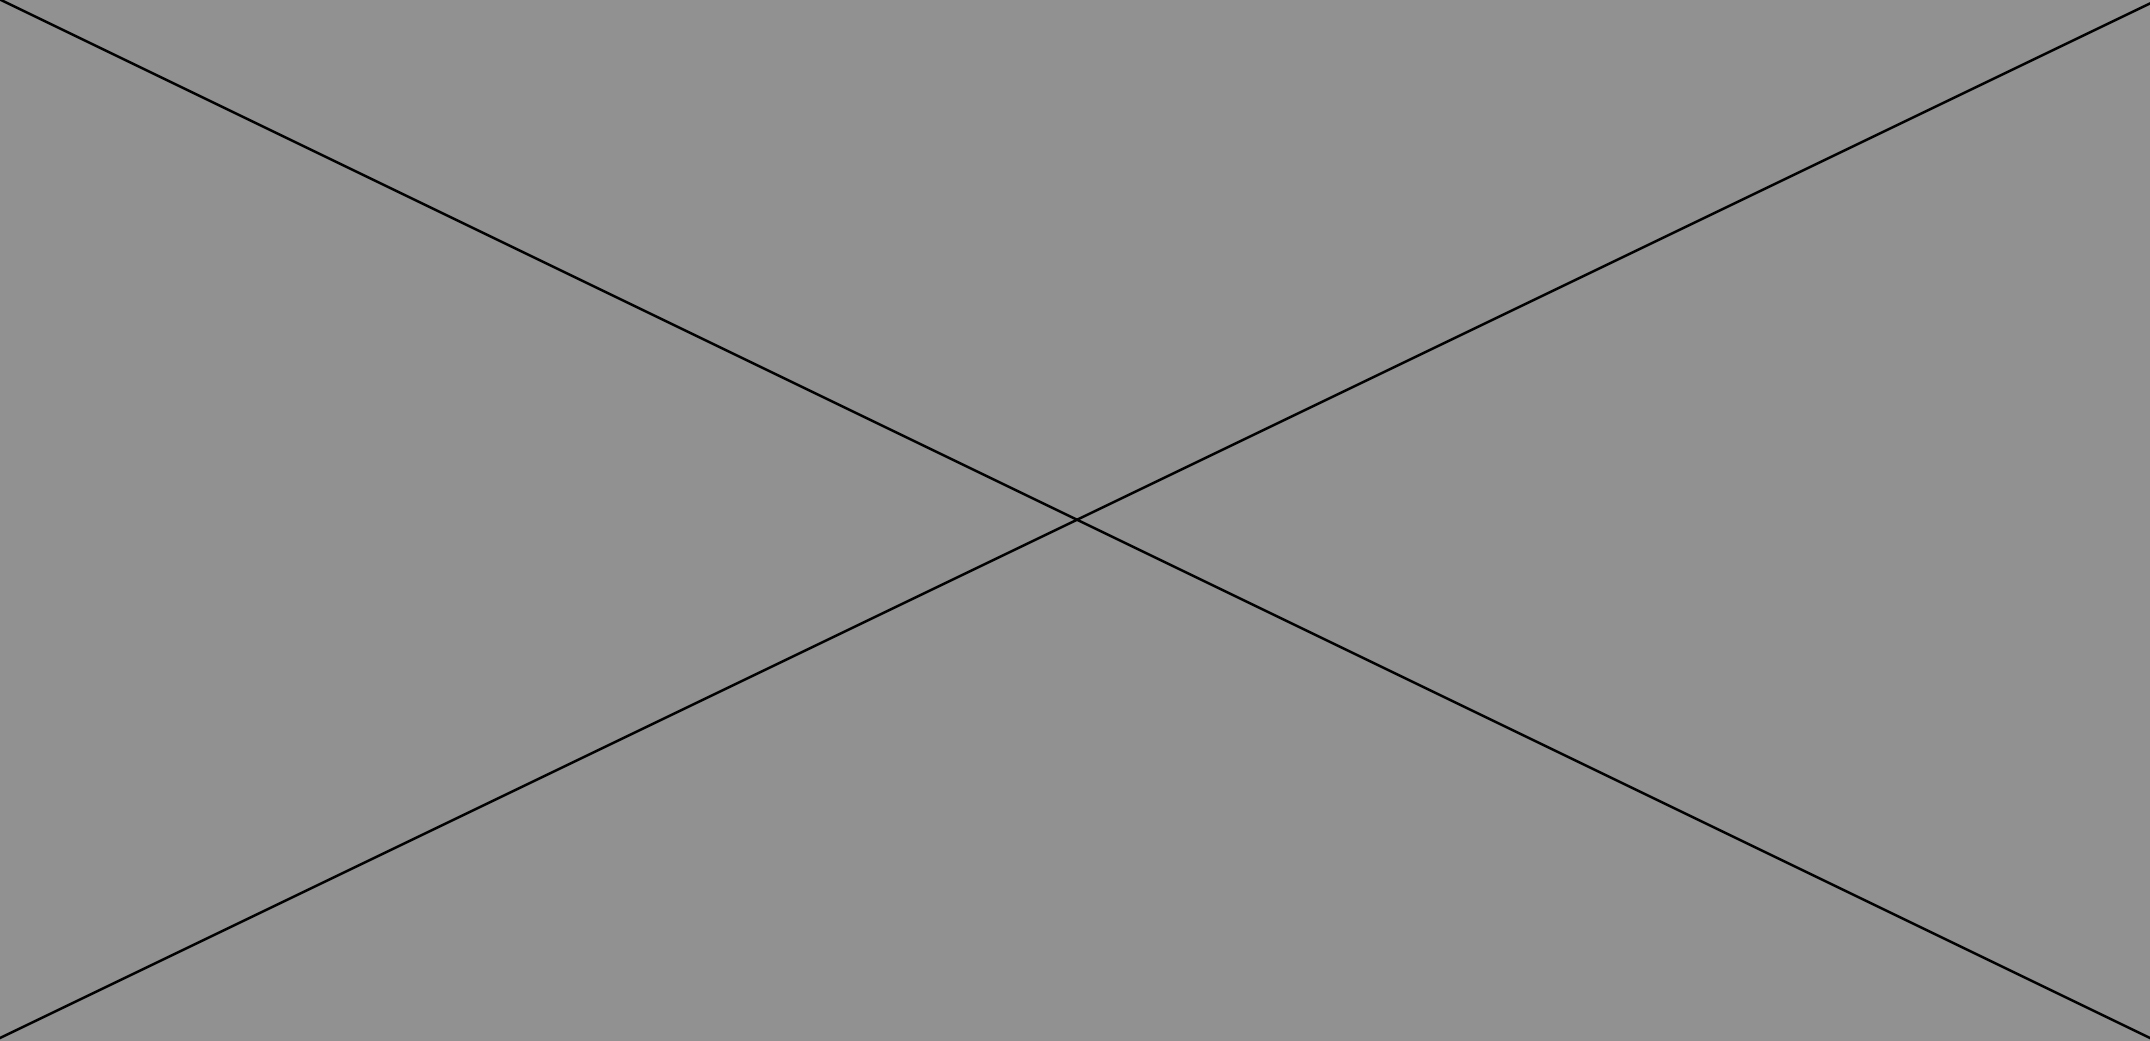
\includegraphics[width=.5\textwidth]{figures/placeholderImg.jpg}
  \caption[P3\_T1 pupil velocity]{P3\_T1 Pupil diameter and eye velocity}
  \label{fig:P3_T1_vel}
\end{figure}

In the only two clear record sets available (Fig.~\ref{fig:P3_T1_vel}), it is possible to see that a number of small saccades with low peaks of velocity are performed during the smooth tracking with a more flat velocity profile. The pattern is visually pretty stable, suggesting a good control over the eye movements performed, regardless their performance.



\subsection{P{1,2,3}\_T2 : Triangular motion visual stimul}
\label{sec:P123_T2}

\subsubsection{P1\_T2}
\label{sec:P1_T2}

\begin{figure}[h]
  \centering
  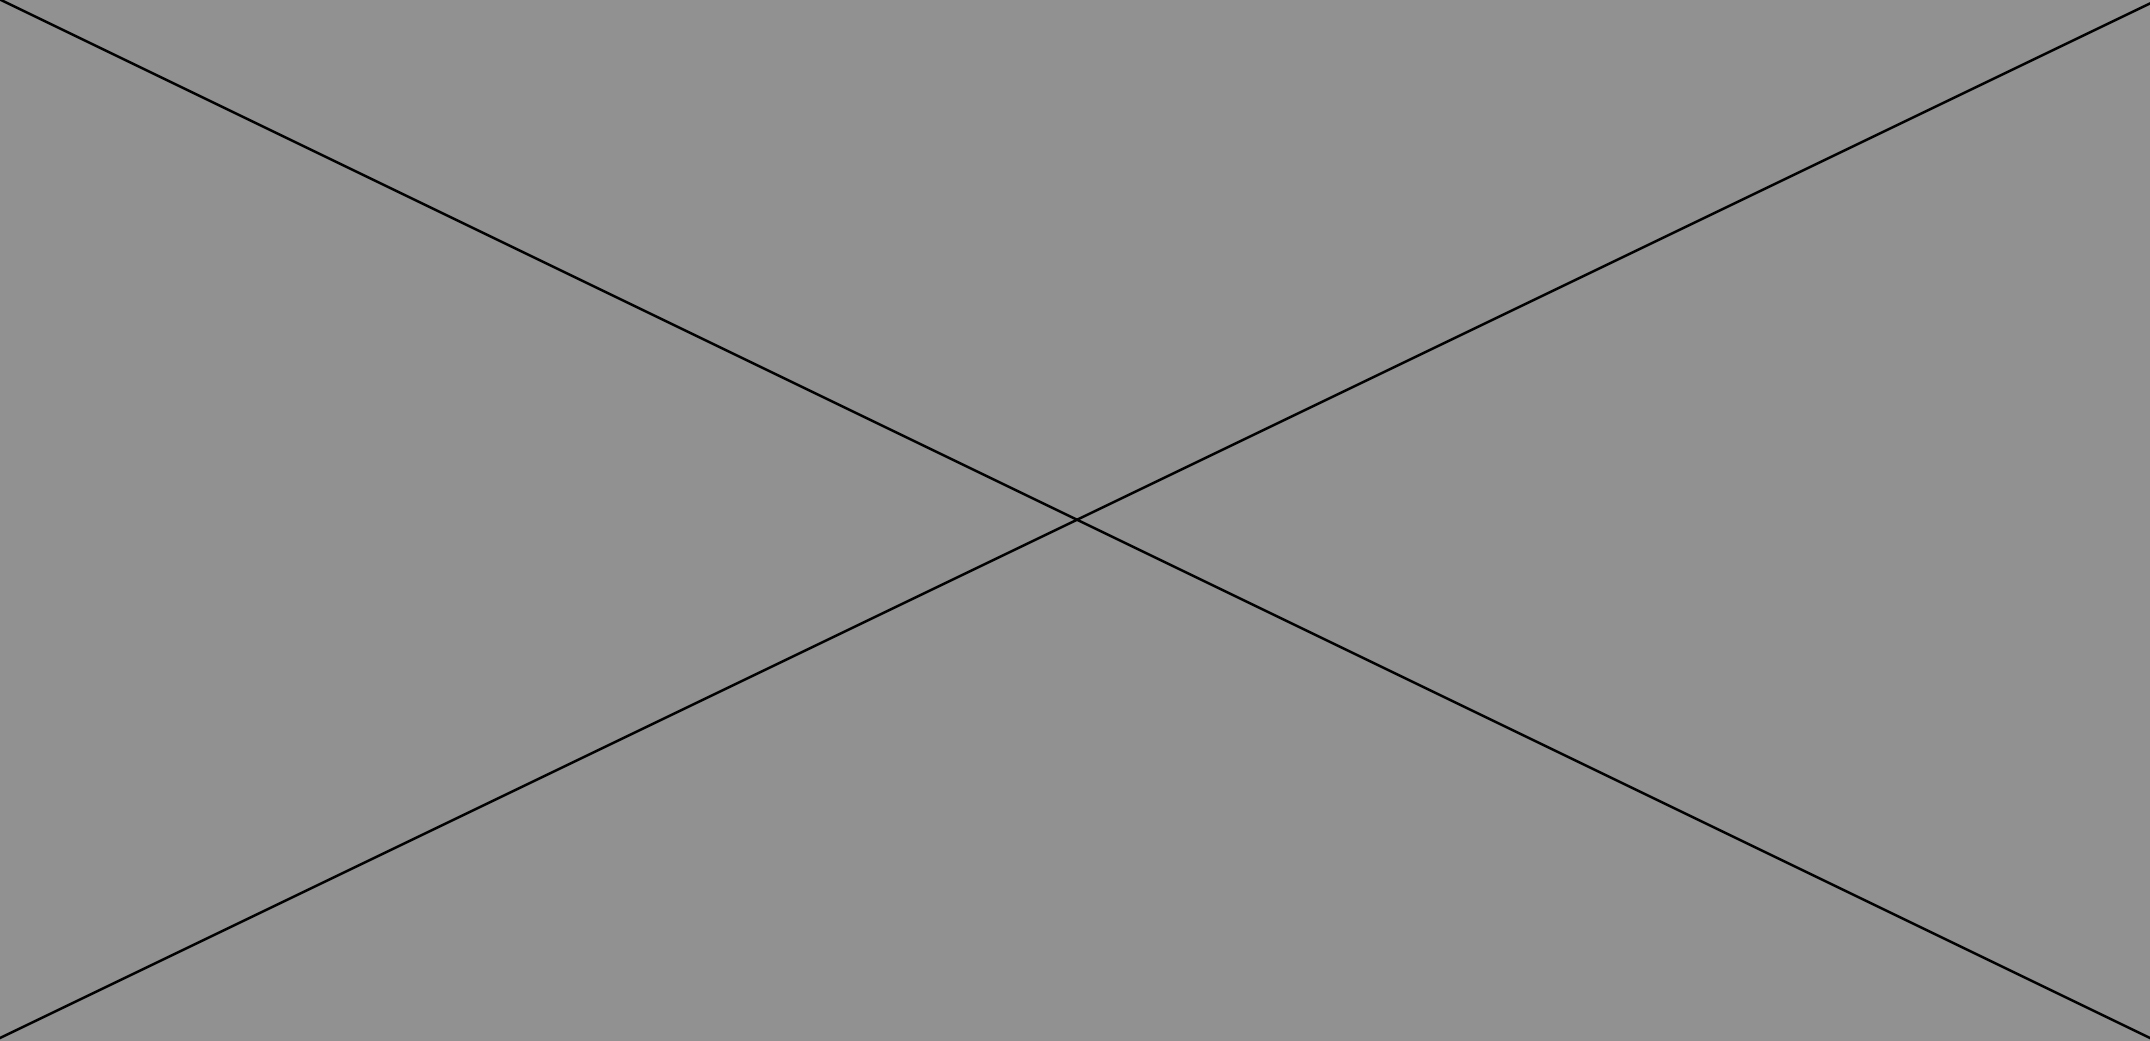
\includegraphics[width=.5\textwidth]{figures/placeholderImg.jpg}
  \caption[P1\_T2 Eye positioning]{P1\_T2 Eye positioning}
  \label{fig:P1_T2_pos}
\end{figure}

In Fig.~\ref{fig:P1_T2_pos} it is possible to spot the triangular motion pattern, however large and small saccades are present throughout the whole record. A couple of full repetitions are clean from saccadic intrusions. The smooth tracking shows a staircase profile, like for the sinusoidal motion stimuli, but it seems less abrupt in this stimuli. This could be due to the fact that the velocity profile of the triangular motion remains constant, resulting in being more predictable and easier to track smoothly for the child.

\begin{figure}[h]
  \centering
  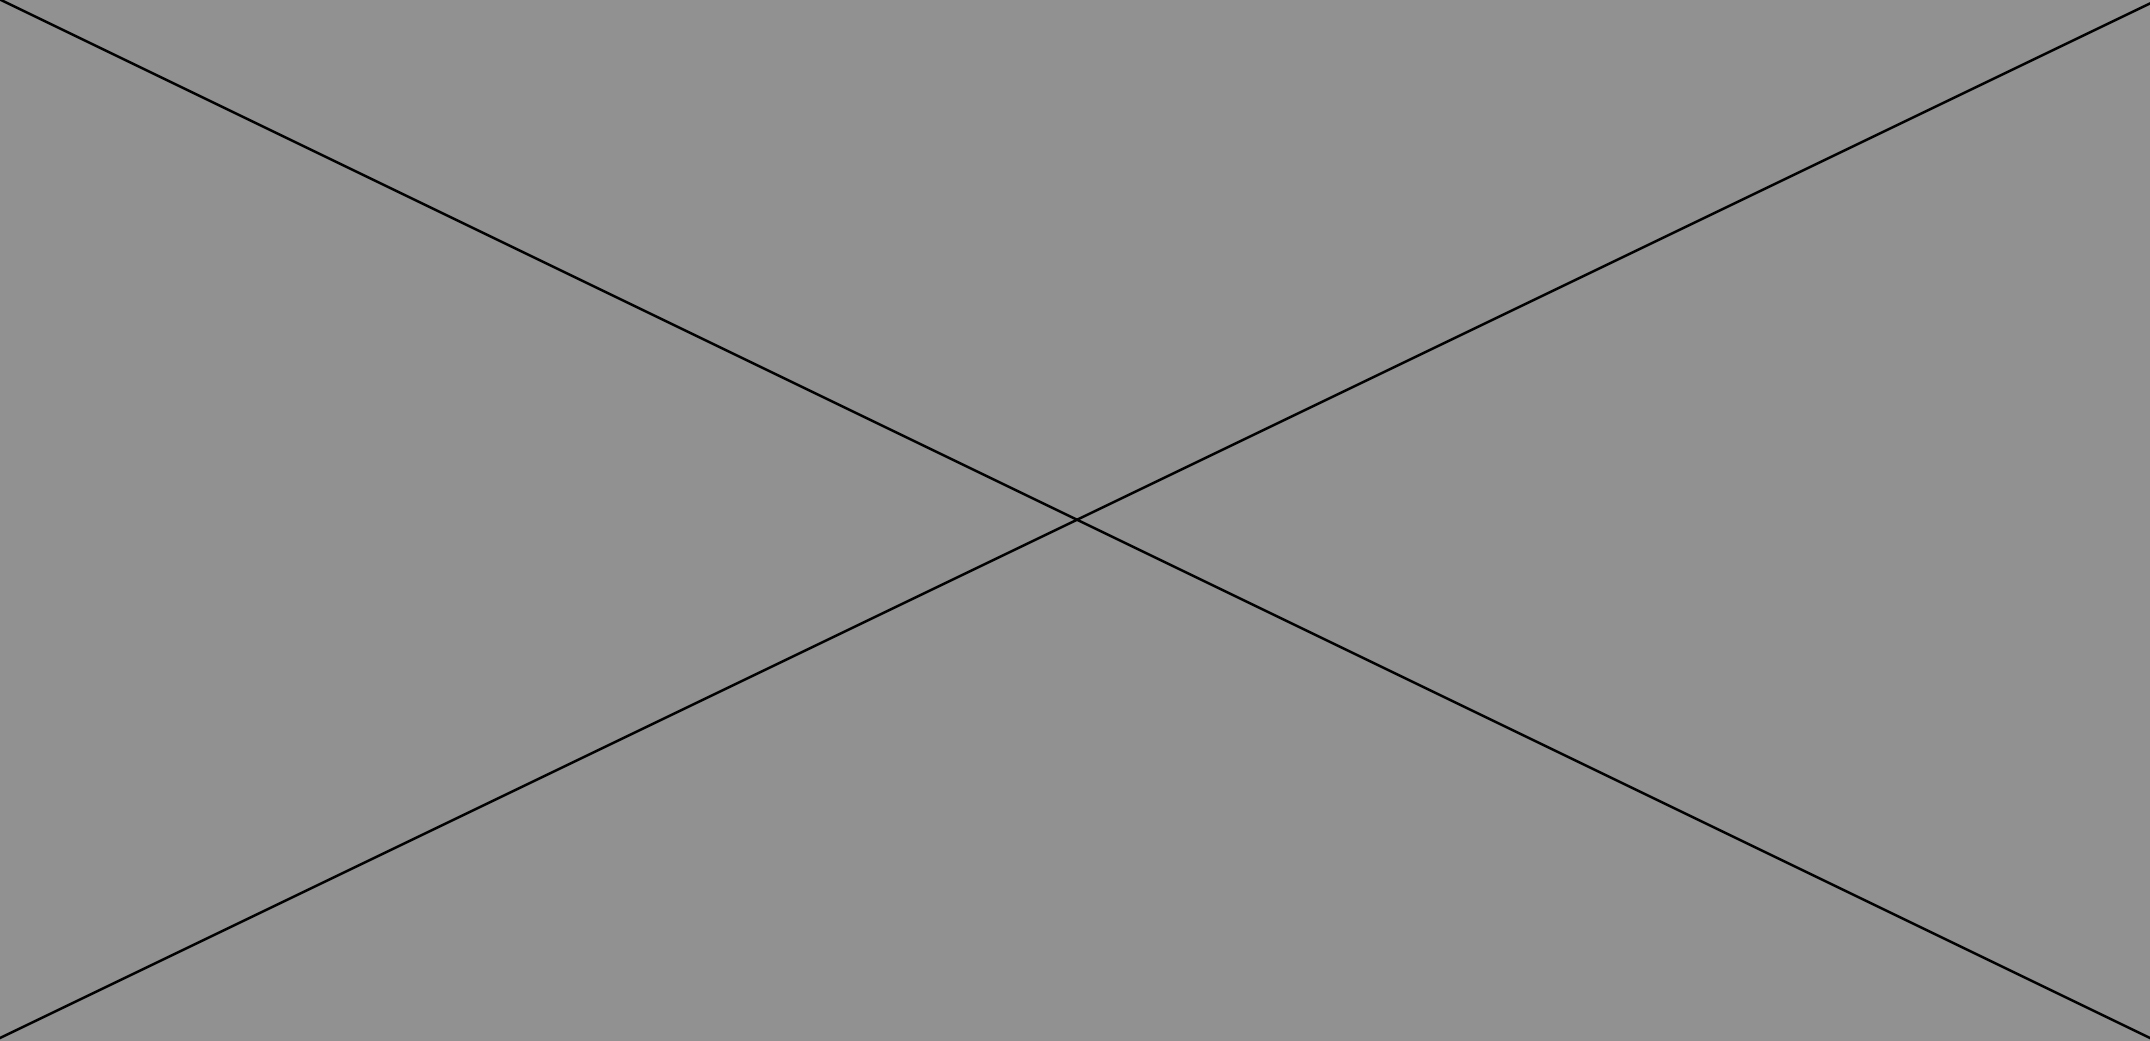
\includegraphics[width=.5\textwidth]{figures/placeholderImg.jpg}
  \caption[P1\_T2 pupil velocity]{P1\_T2 Pupil diameter and eye velocity}
  \label{fig:P1_T2_vel}
\end{figure}

Fig.~\ref{fig:P1_T2_vel} shows the presence of small saccades intruding the smooth pursuit even in the two cleaner repetitions.


\subsubsection{P2\_T2}
\label{sec:P2_T2}

\begin{figure}[h]
  \centering
  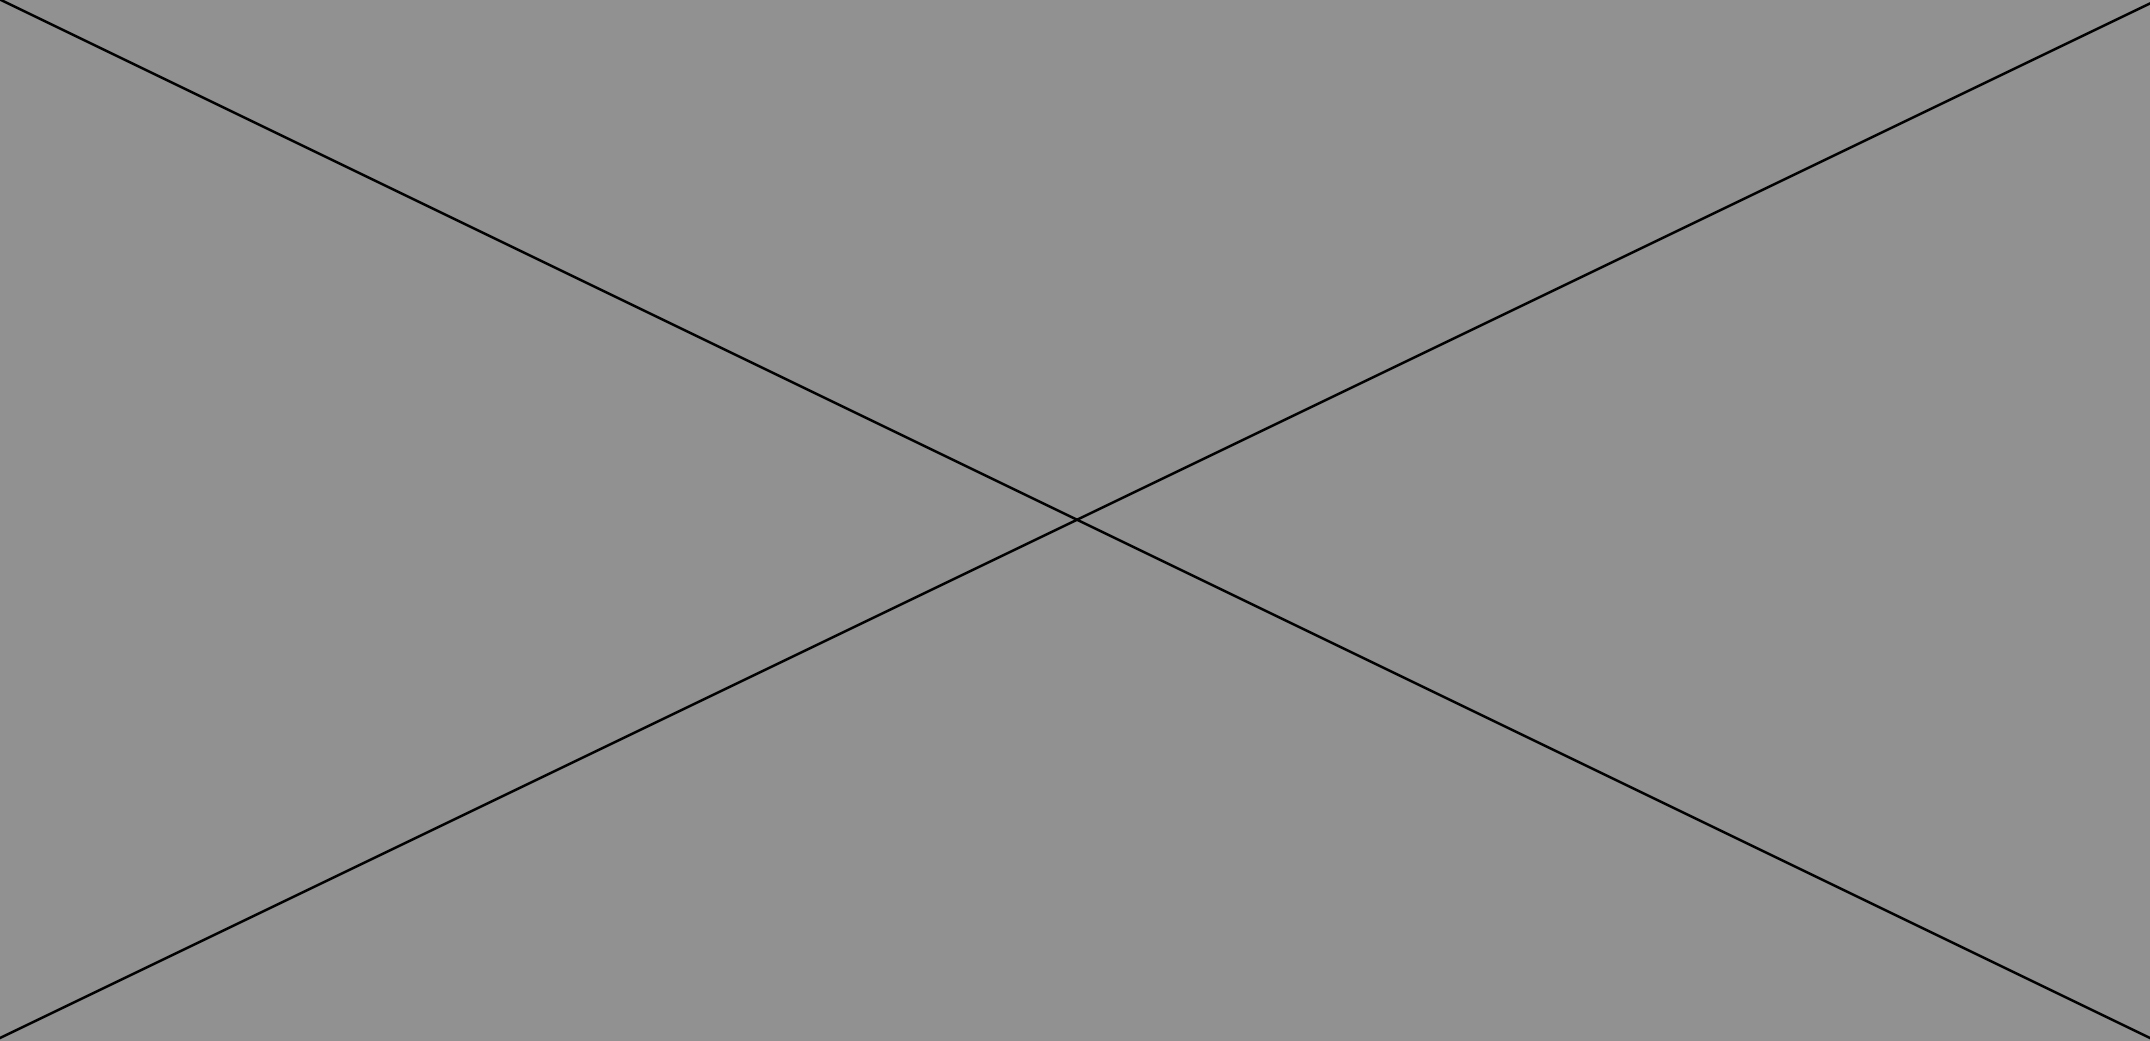
\includegraphics[width=.5\textwidth]{figures/placeholderImg.jpg}
  \caption[P1\_T2 Eye positioning]{P2\_T2 Eye positioning}
  \label{fig:P2_T2_pos}
\end{figure}

The graph for the triangular pursuit of P2 (Fig.~\ref{fig:P2_T2_pos})  is particularly rich of artifacts, which are particularly irregular and therefore probably due more to movements of the head or the whole body of the child rather than being caused by only by eye movements. Indeed, the dense repetition of quick eye movements, starting from the second repetition of the triangular wave, can be better explained by the child trying to track the object while keeping moving on the lap of her mother. In the record of the first clean repetition of the stimuli it is possible to see that the smooth tracking is pretty precise for the y coordinate of the eye, while the left eye leads the right one in terms of x coordinate. This might be due to the fact that the child’s head was a bit tilted or the calibration was not precise due to the movements of the child. Overall, the record does not seem to provide many reliable measurements for smooth pursuit eye movements. It is possible that the stimuli was not different enough from the previous one in order to be interesting enough for the child, or she felt uncomfortable to sit still in position at the moment of this trial.

\begin{figure}[h]
  \centering
  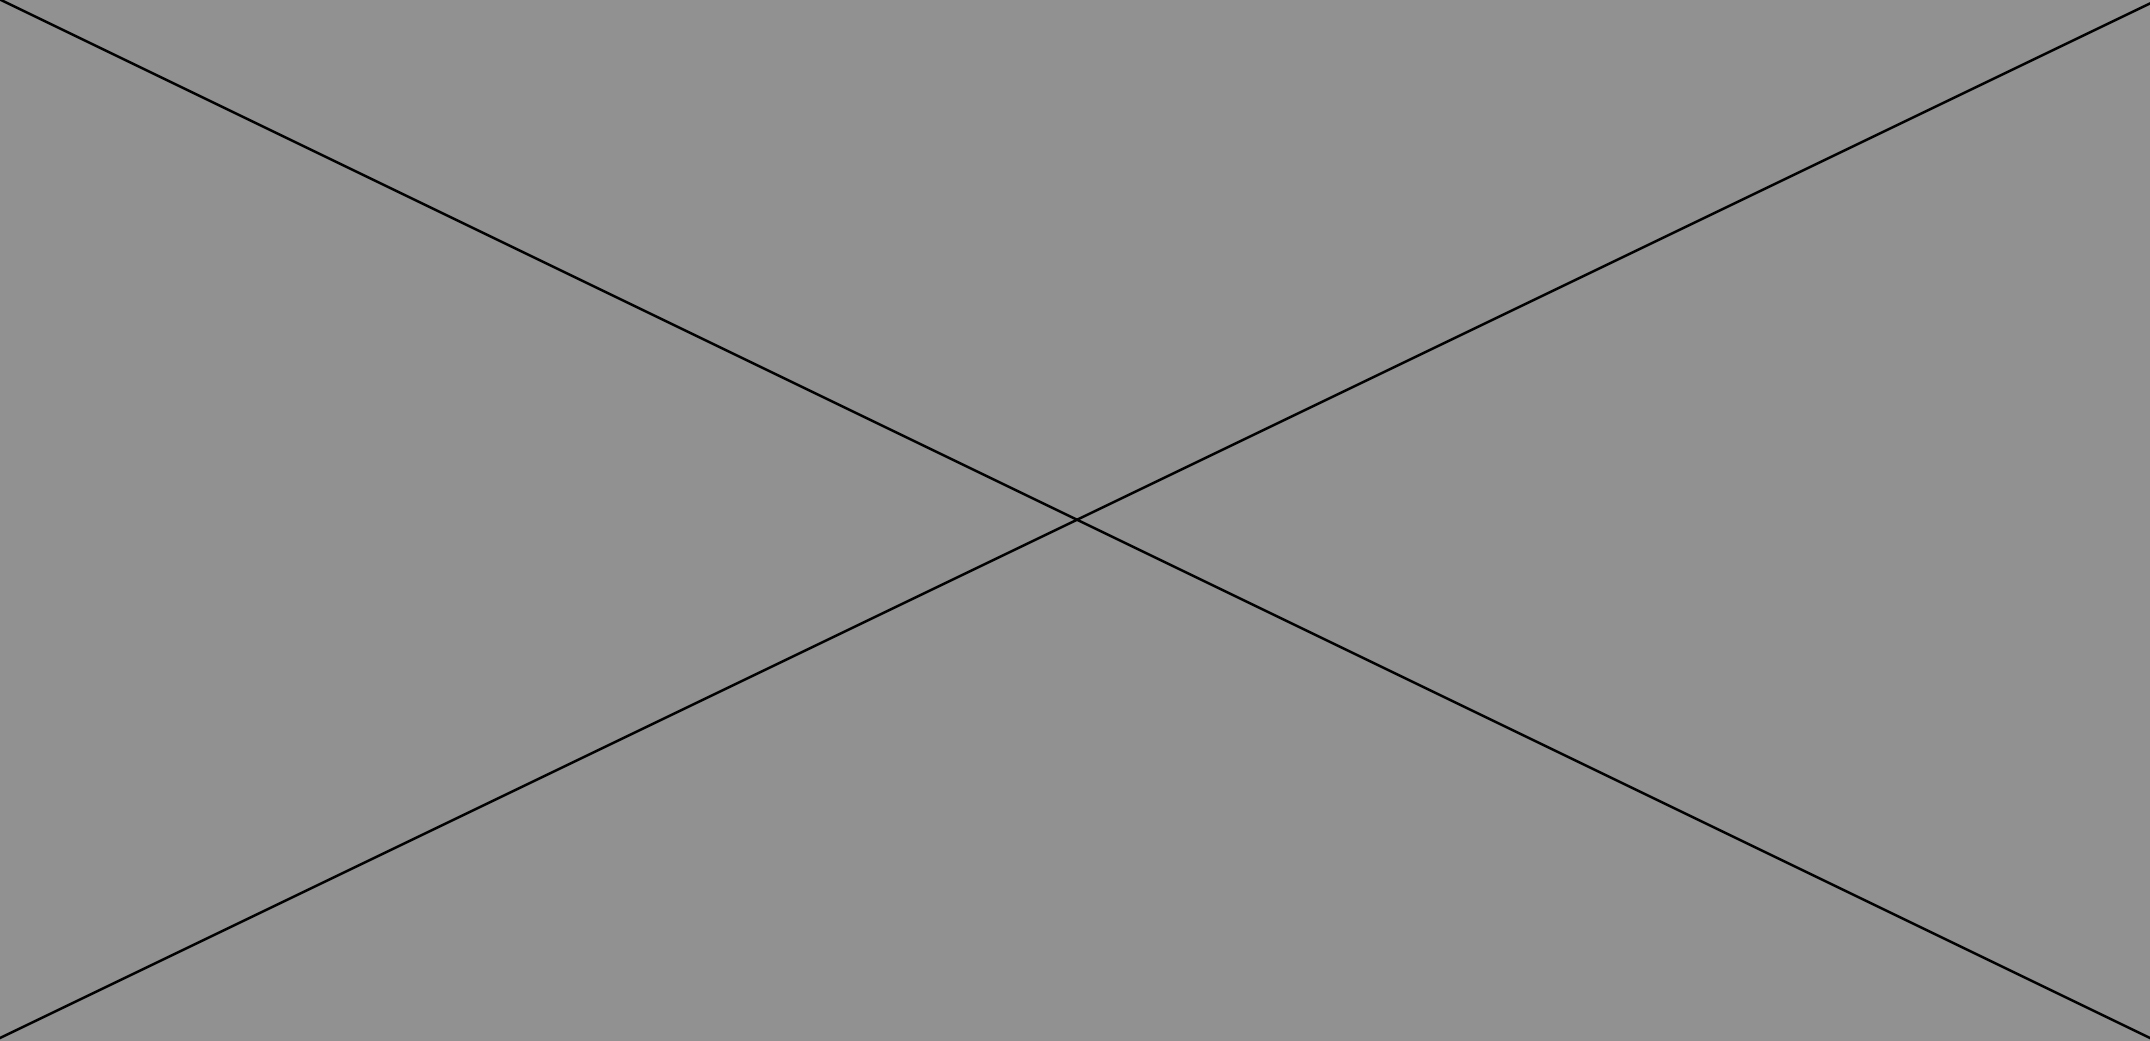
\includegraphics[width=.5\textwidth]{figures/placeholderImg.jpg}
  \caption[P2\_T2 pupil velocity]{P2\_T2 Pupil diameter and eye velocity}
  \label{fig:P2_T2_vel}
\end{figure}

Fig.~\ref{fig:P2_T2_vel} shows how only the first repetition of the stimuli shows eye tracking with a velocity profile clean an flat enough to be considered smooth pursuit. The rest of the record is too noisy to be considered.




\subsubsection{P3\_T2}
\label{sec:P3_T2}

\begin{figure}[h]
  \centering
  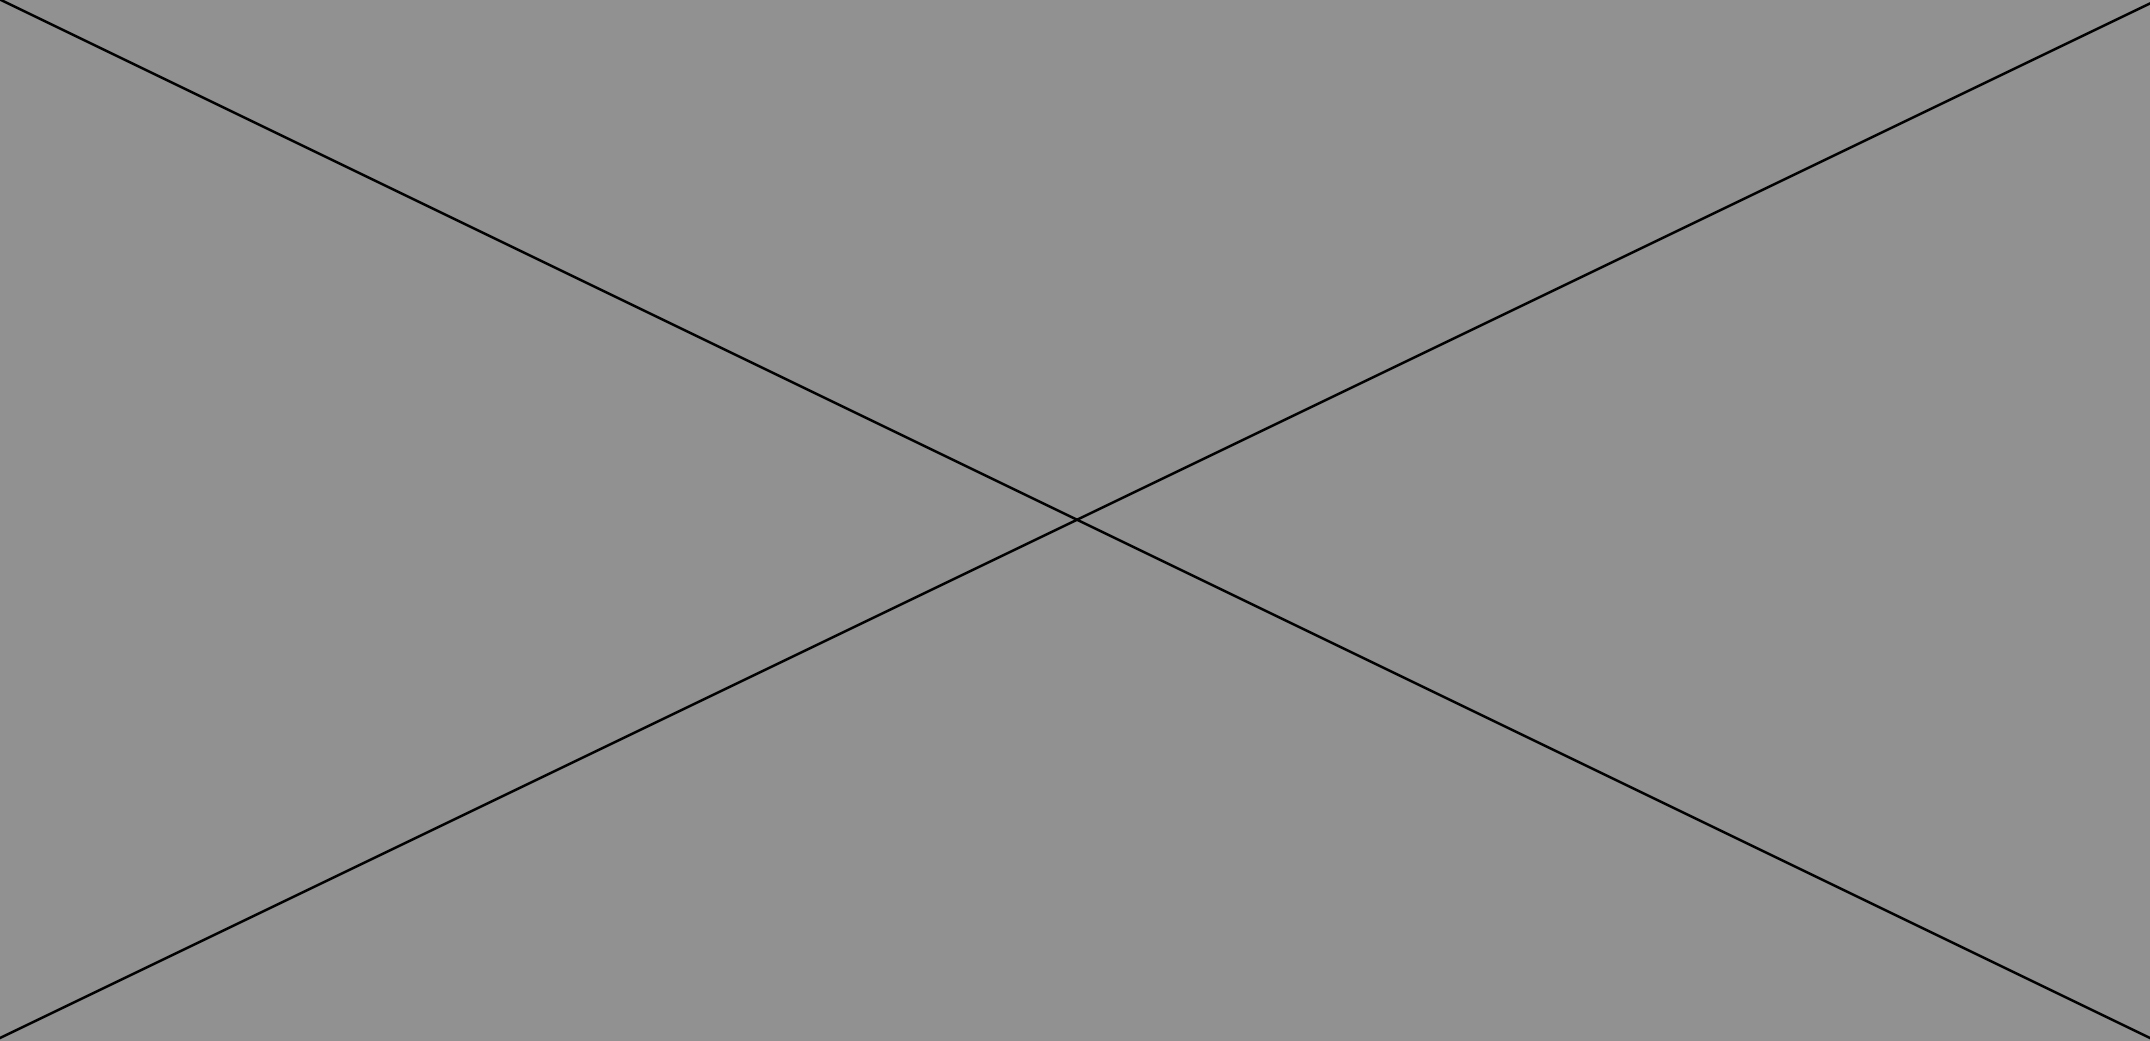
\includegraphics[width=.5\textwidth]{figures/placeholderImg.jpg}
  \caption[P3\_T2 Eye positioning]{P3\_T2 Eye positioning}
  \label{fig:P3_T2_pos}
\end{figure}

The tracking record of P3 (Fig.~\ref{fig:P3_T2_pos}) is pretty accurate, she followed the stimuli mainly during the second part of the presentation. Large saccades are visible at the target turning points, as predictable, both on the horizontal and vertical axes. A staircase profile for the smooth tracking is present also in this stimuli. Overall the stimuli seemed to work  well in eliciting the expected gaze pattern. The central part of the record is missing, probably because the child looked away for some time.

\begin{figure}[h]
  \centering
  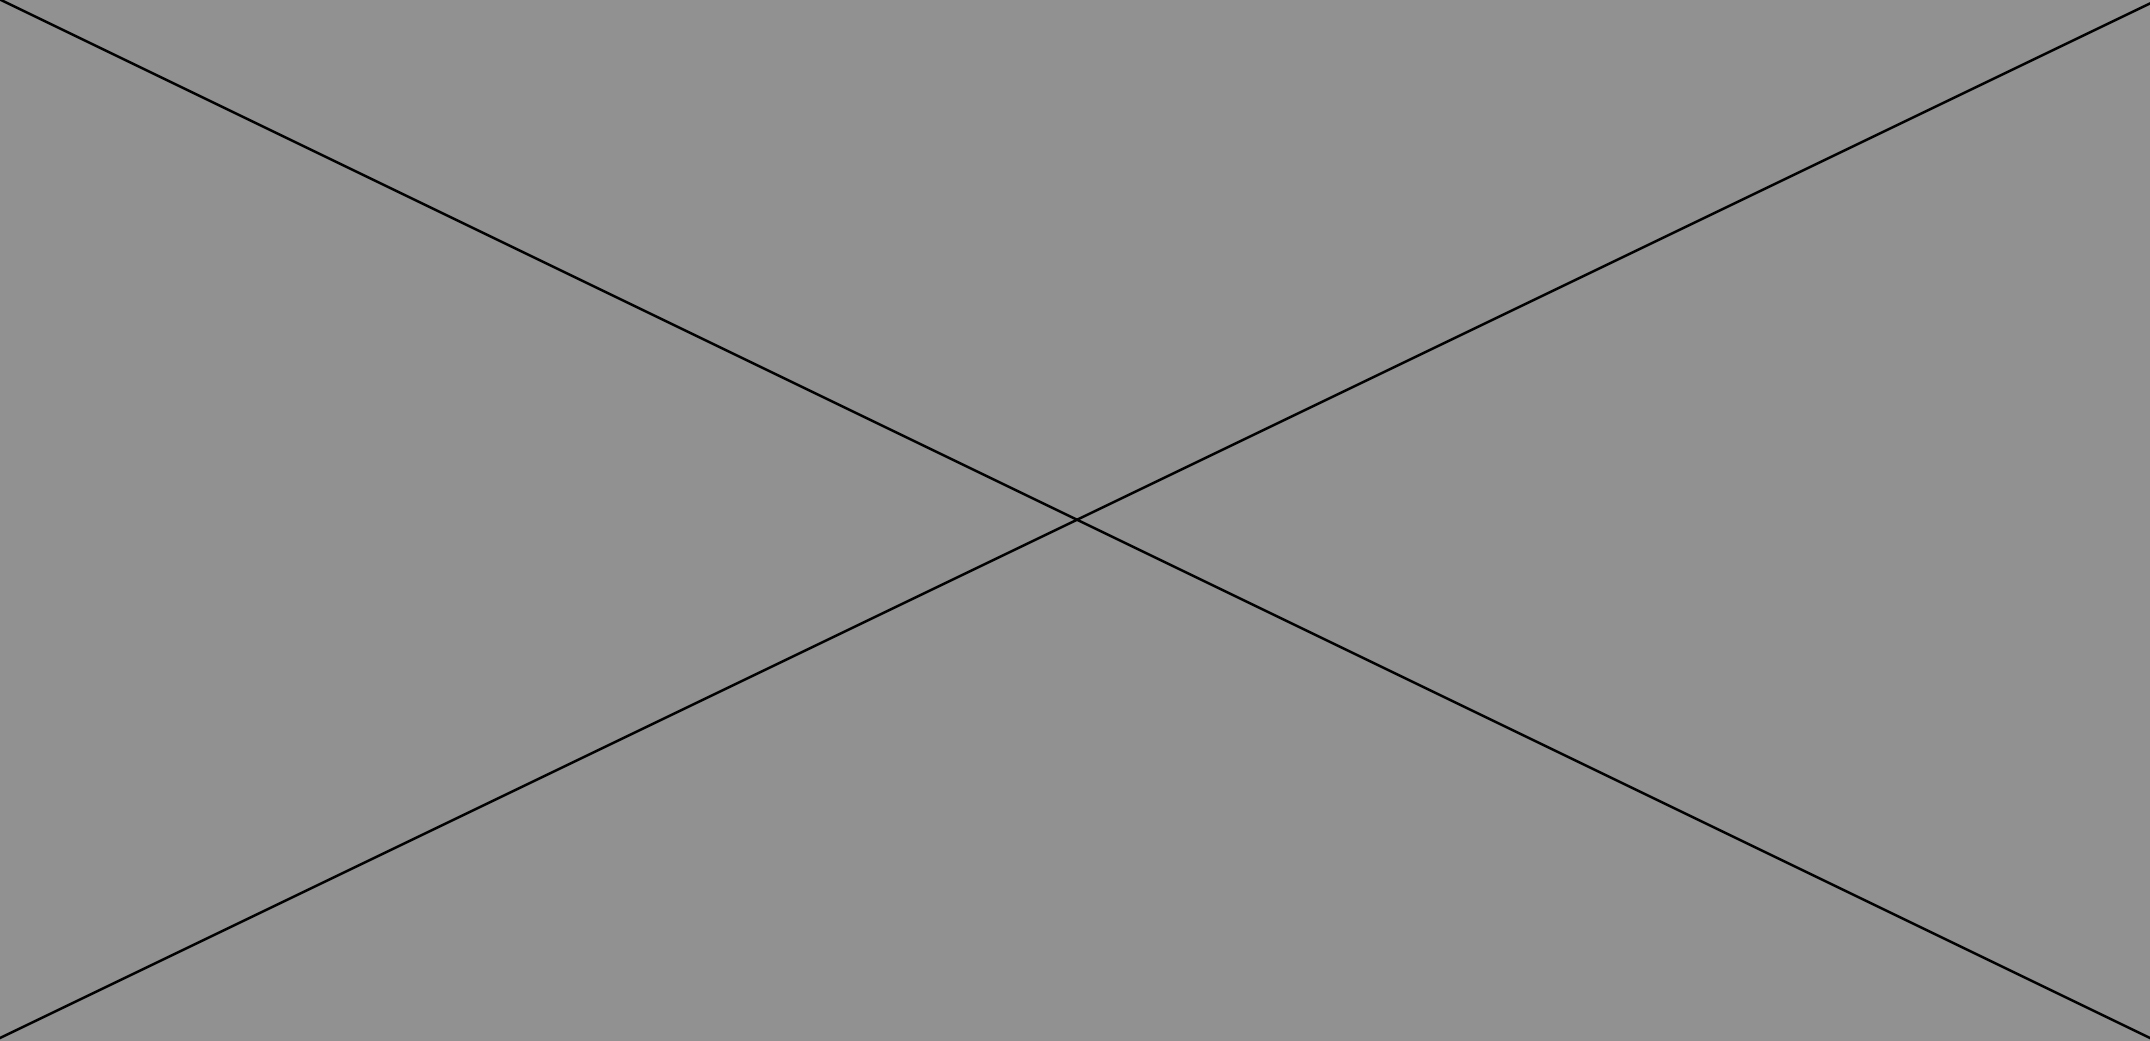
\includegraphics[width=.5\textwidth]{figures/placeholderImg.jpg}
  \caption[P3\_T2 pupil velocity]{P3\_T2 Pupil diameter and eye velocity}
  \label{fig:P3_T2_vel}
\end{figure}

Fig.~\ref{fig:P3_T2_vel} shows how in the first repetition of the stimuli few saccades with small peaks in velocity disrupted an otherwise pretty flat eye velocity profile, suggesting smooth tracking. On the other hand, In the second part of the stimuli more and larger saccades intruded the smooth tracking.



\subsubsection{P1\_T3}
\label{sec:P1_T3}

\begin{figure}[h]
  \centering
  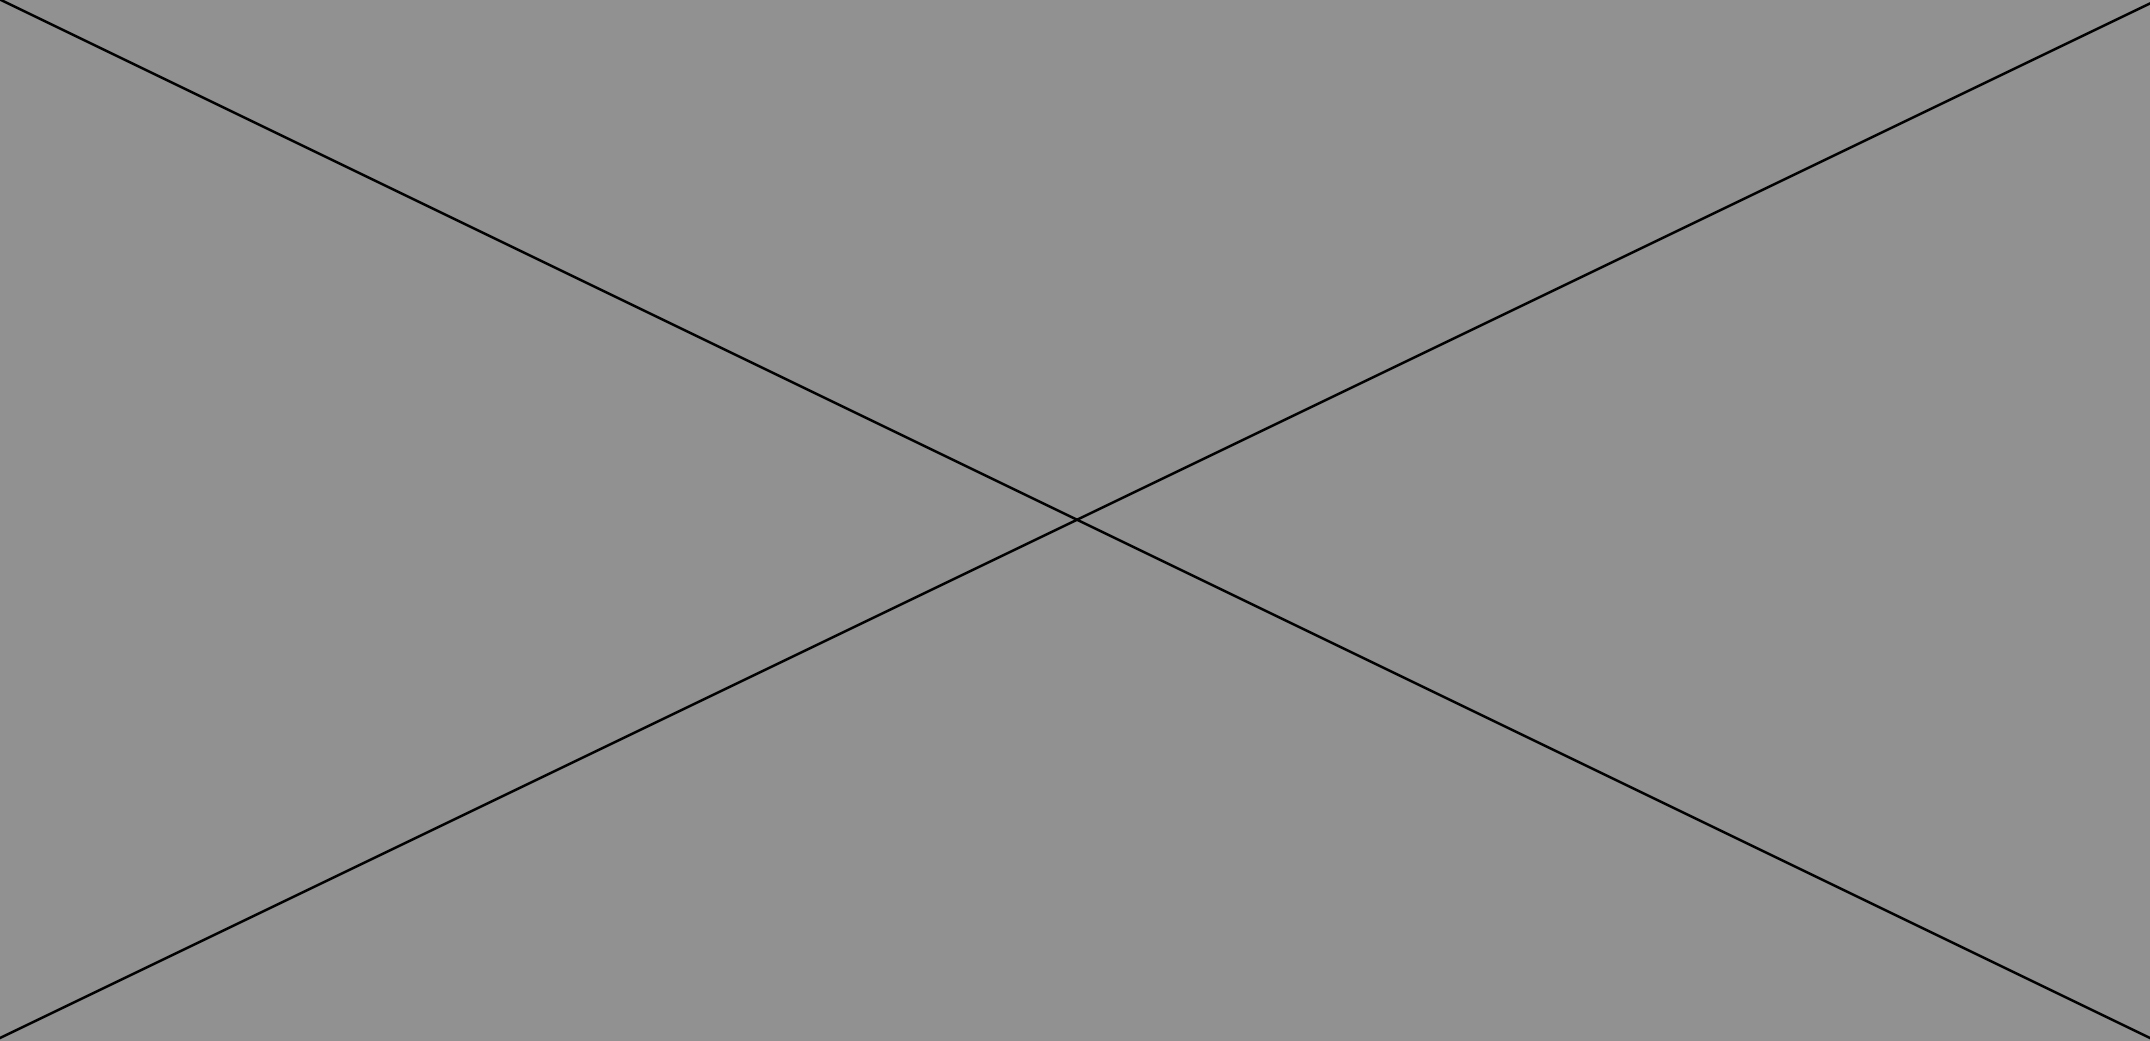
\includegraphics[width=.5\textwidth]{figures/placeholderImg.jpg}
  \caption[P1\_T3 Eye positioning]{P1\_T3 Eye positioning}
  \label{fig:P1_T3_pos}
\end{figure}

Fig.~\ref{fig:P1_T3_pos} shows pretty clearly that the stimuli elicited the expected eye movements. All the phases of the paradigm are easily detectable (initial \textit{fixation}, \textit{step} saccade, smooth pursuit \textit{ramp}). A number of large saccade is visible, happening in particular moments (e.g. during the step, or when the target returns to the central point after the end of a repetition). Some of them might be also blinks, since they happen in the middle of pursuit tracking, where no competing stimuli or abrupt target movements are shown. The tracking appears accurate, and the staircase pattern is visible only in some parts of the chart.

\begin{figure}[h]
  \centering
  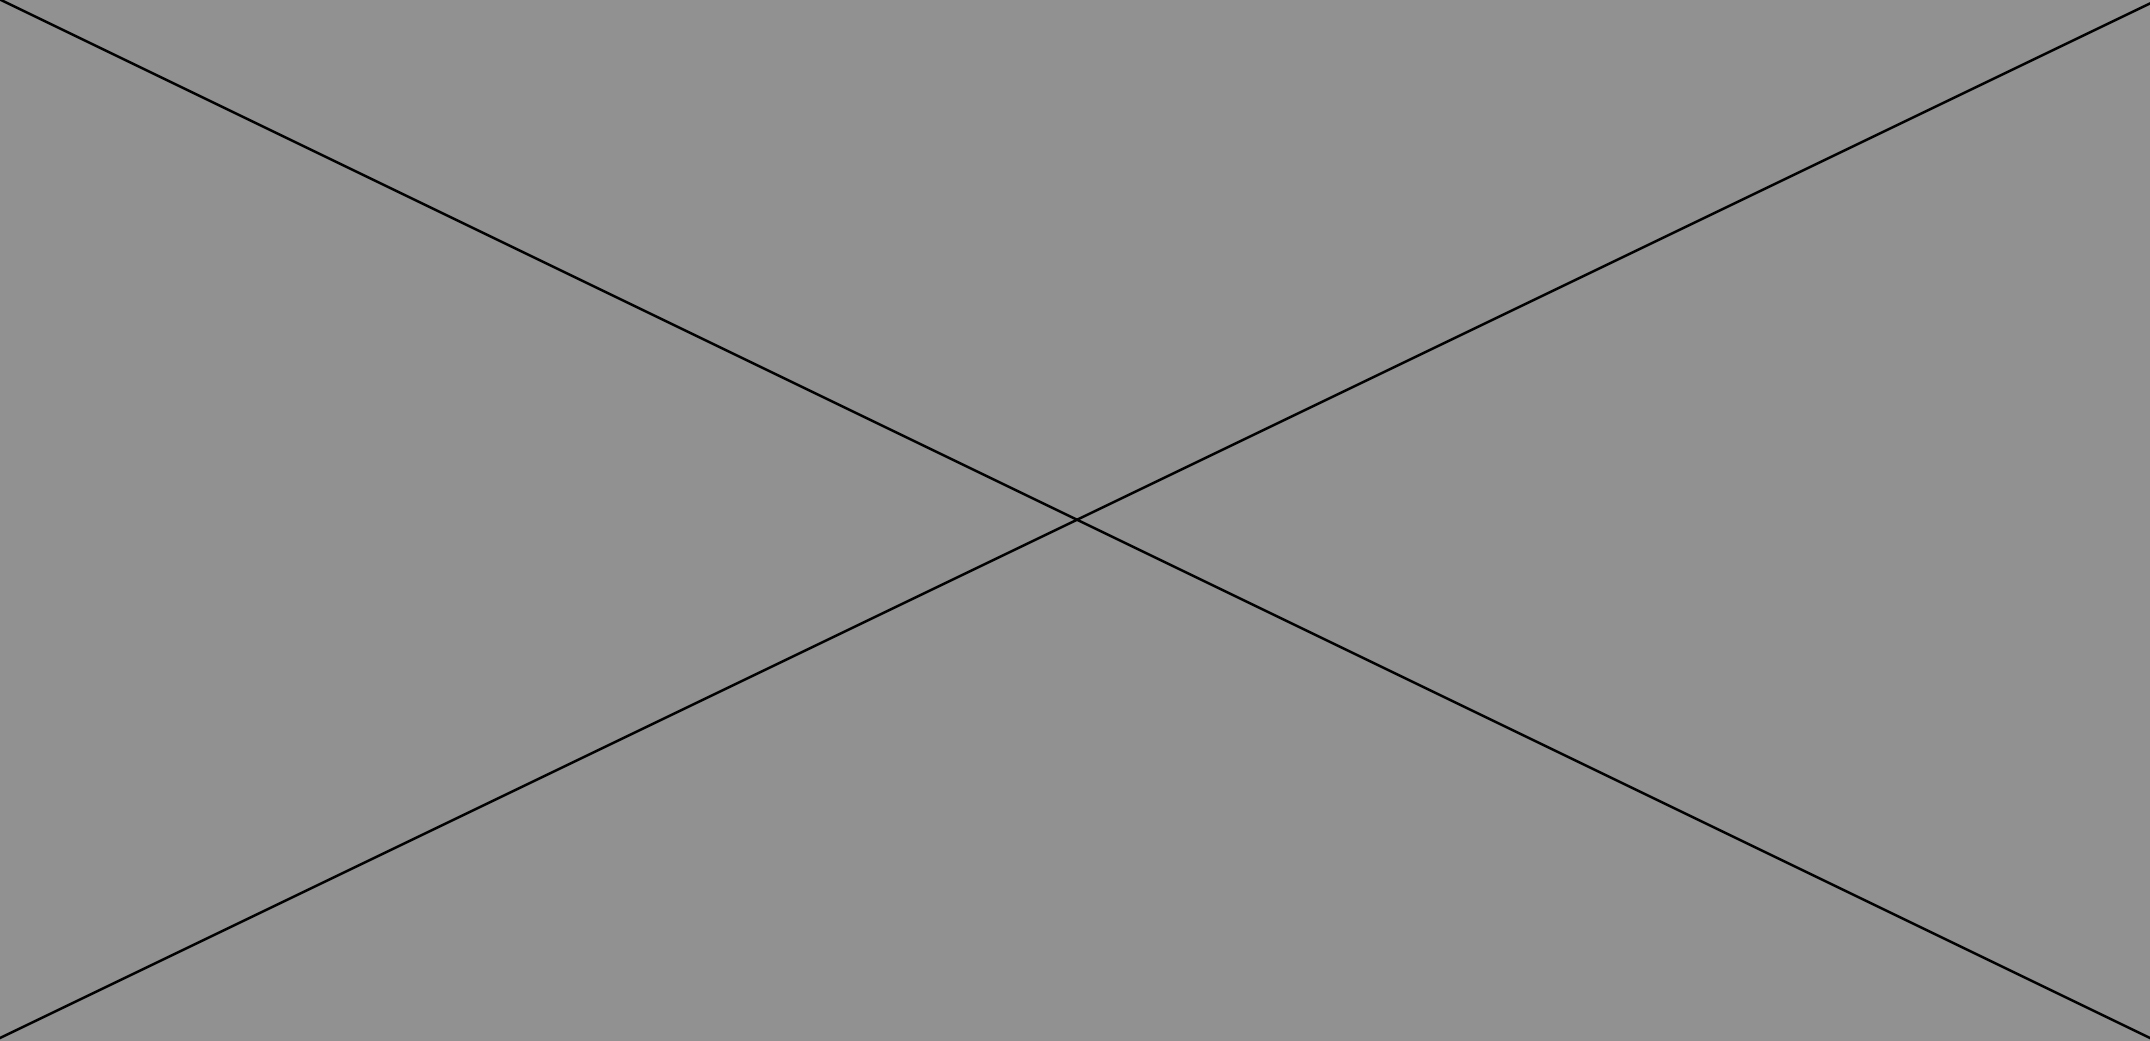
\includegraphics[width=.5\textwidth]{figures/placeholderImg.jpg}
  \caption[P1\_T3 pupil velocity]{P1\_T3 Pupil diameter and eye velocity}
  \label{fig:P1_T3_vel}
\end{figure}

Fig.~\ref{fig:P1_T3_vel} shows the presence of a series of saccades with consistent velocity, around 400 deg/s, which happen at during the step phase. The other larger saccades with higher peaks of velocity can be considered as intrusive of either fixations or smooth pursuit. The velocity profile, when not disrupted by saccades, appears fairly flat, indicating somewhat stable fixations and smooth pursuits. 



\subsubsection{P2\_T3}
\label{sec:P2_T3}

The eye tracking data of P2 during the step-ramp visual stimuli are insufficient for being analyzed (Fig.~\ref{fig:P2_T3_pos}; Fig.~\ref{fig:P2_T3_vel}). Indeed, at this point of the experiment P2 seemed tired of watching at the display monitor. Probably the experiment was lasting for too long, and she lost interest. Indeed, the researchers and P2’s mother decided to stop the experiment and leave the child to go outside to play with her friends. P2 did not perform further trials.

\begin{figure}[h]
  \centering
  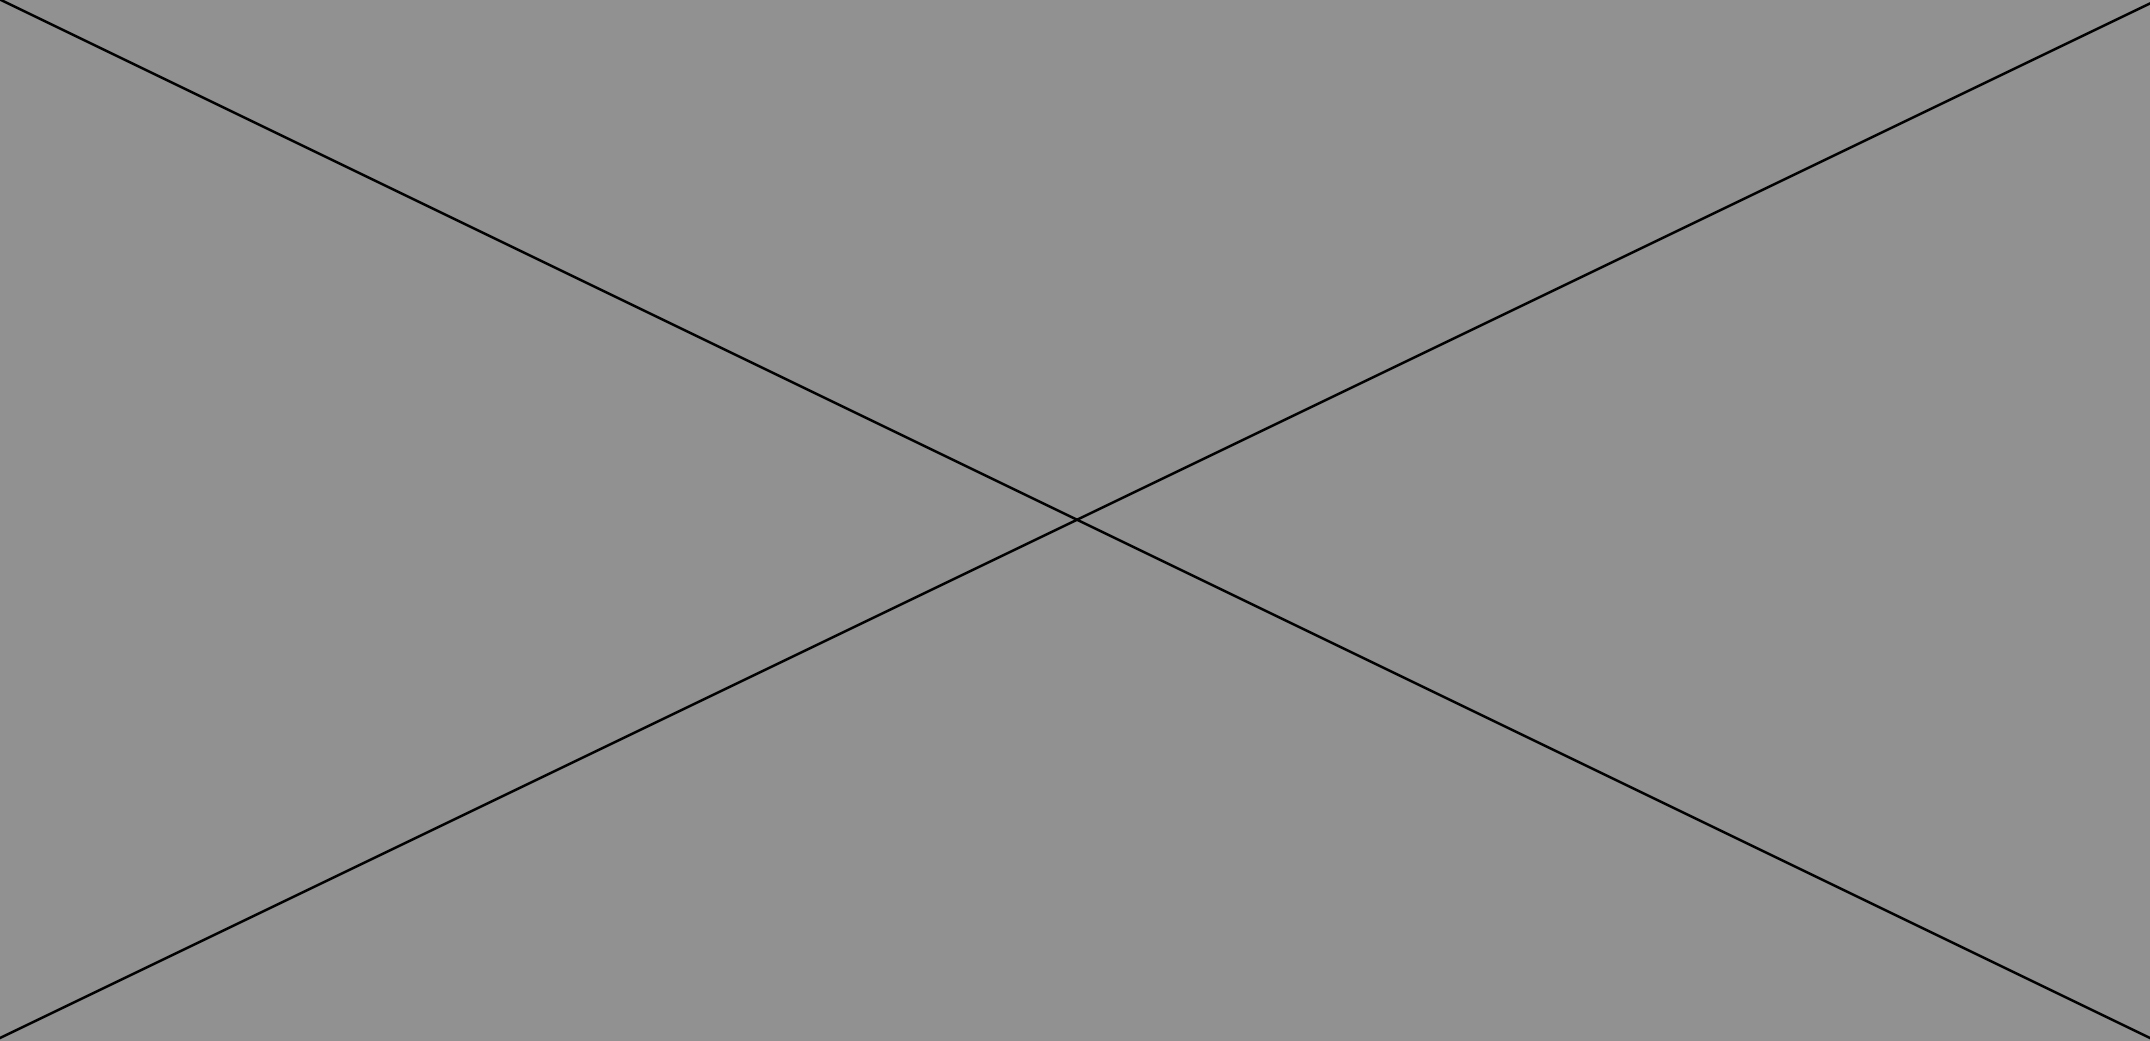
\includegraphics[width=.5\textwidth]{figures/placeholderImg.jpg}
  \caption[P2\_T3 Eye positioning]{P2\_T3 Eye positioning}
  \label{fig:P2_T3_pos}
\end{figure}

\begin{figure}[h]
  \centering
  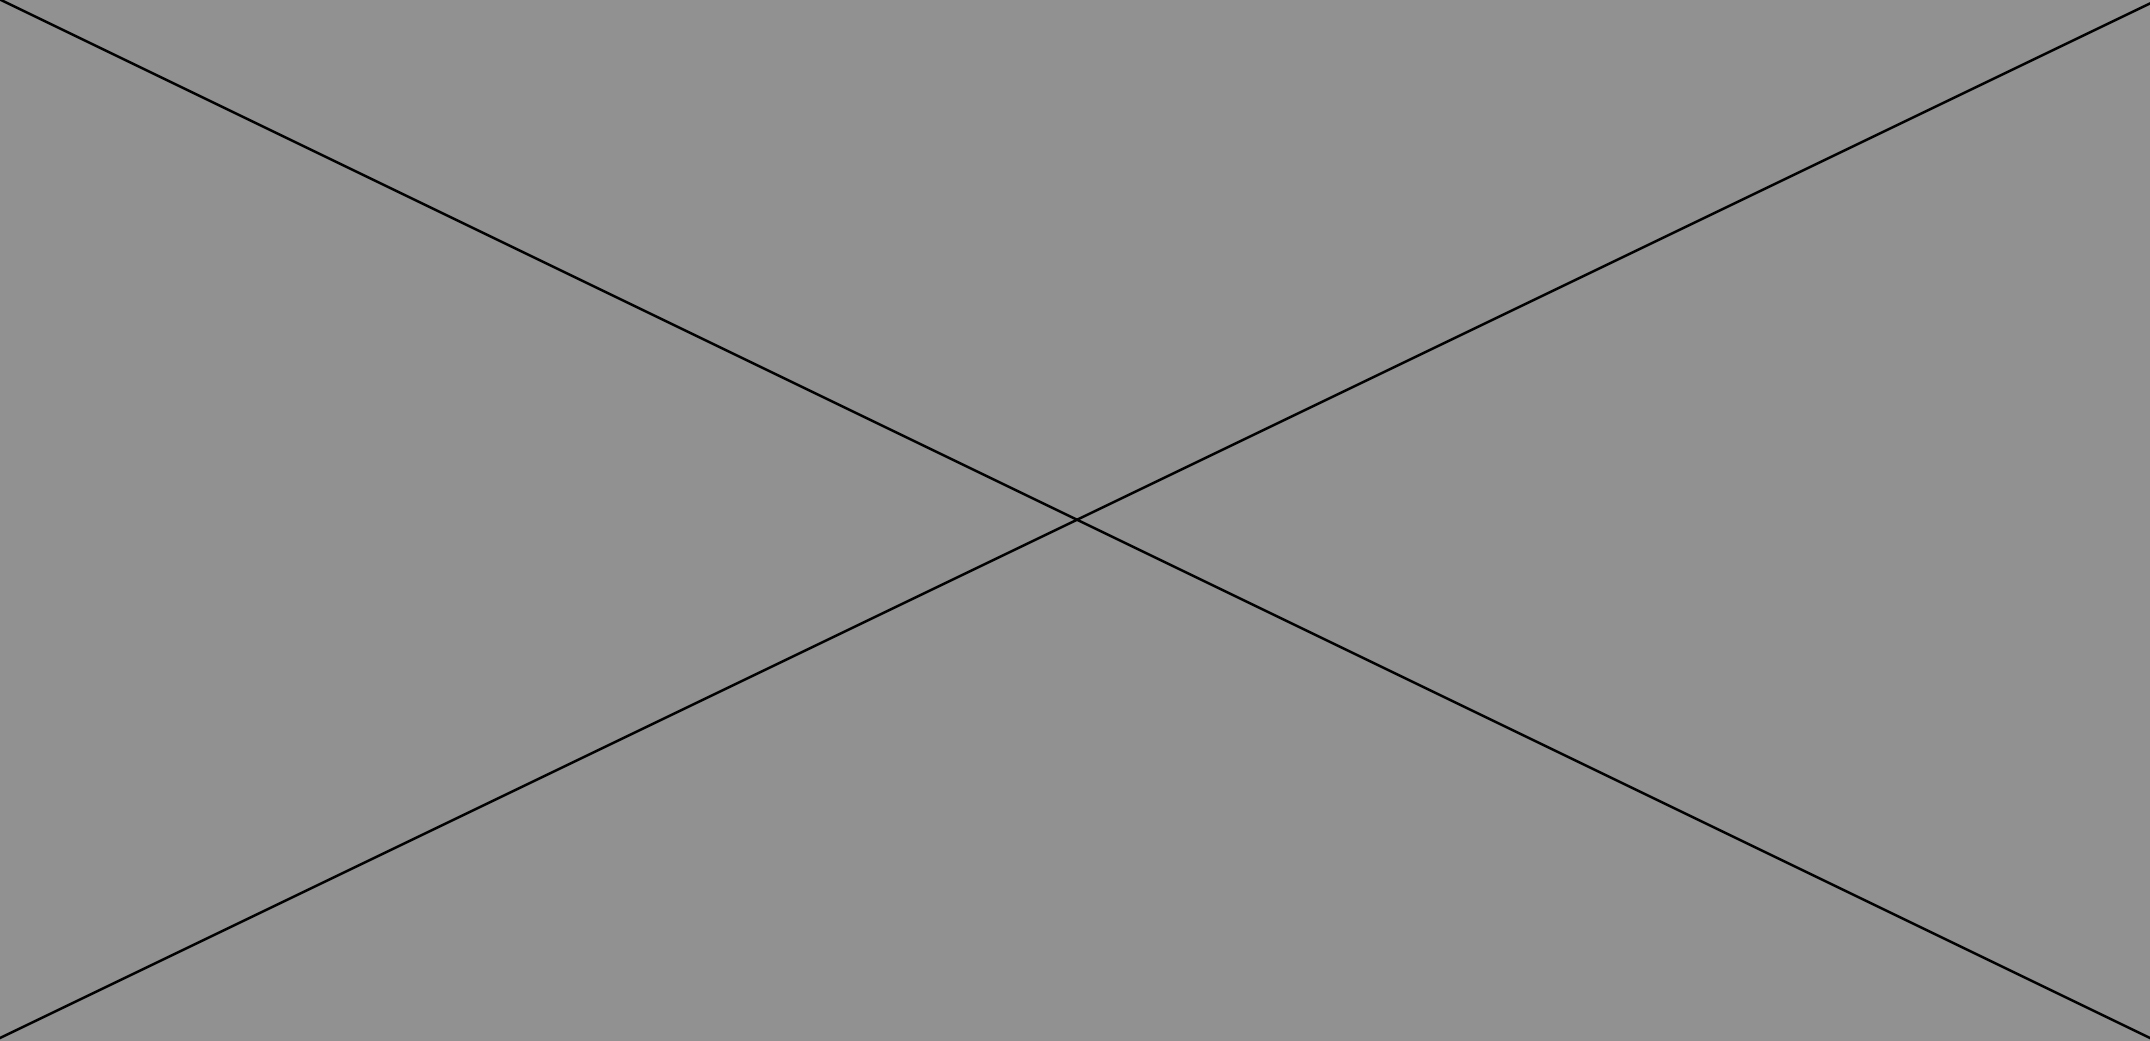
\includegraphics[width=.5\textwidth]{figures/placeholderImg.jpg}
  \caption[P2\_T3 pupil velocity]{P2\_T3 Pupil diameter and eye velocity}
  \label{fig:P2_T3_vel}
\end{figure}


\subsubsection{P3\_T3}
\label{sec:P3_T3}

The record for the step-ramp stimuli of P3 stops after the second repetition. After that moment, P3 started interacting with her sister and her mother. She was probably a bit tired to look at the display monitor too. However, the recorded data show interesting patterns.

\begin{figure}[h]
  \centering
  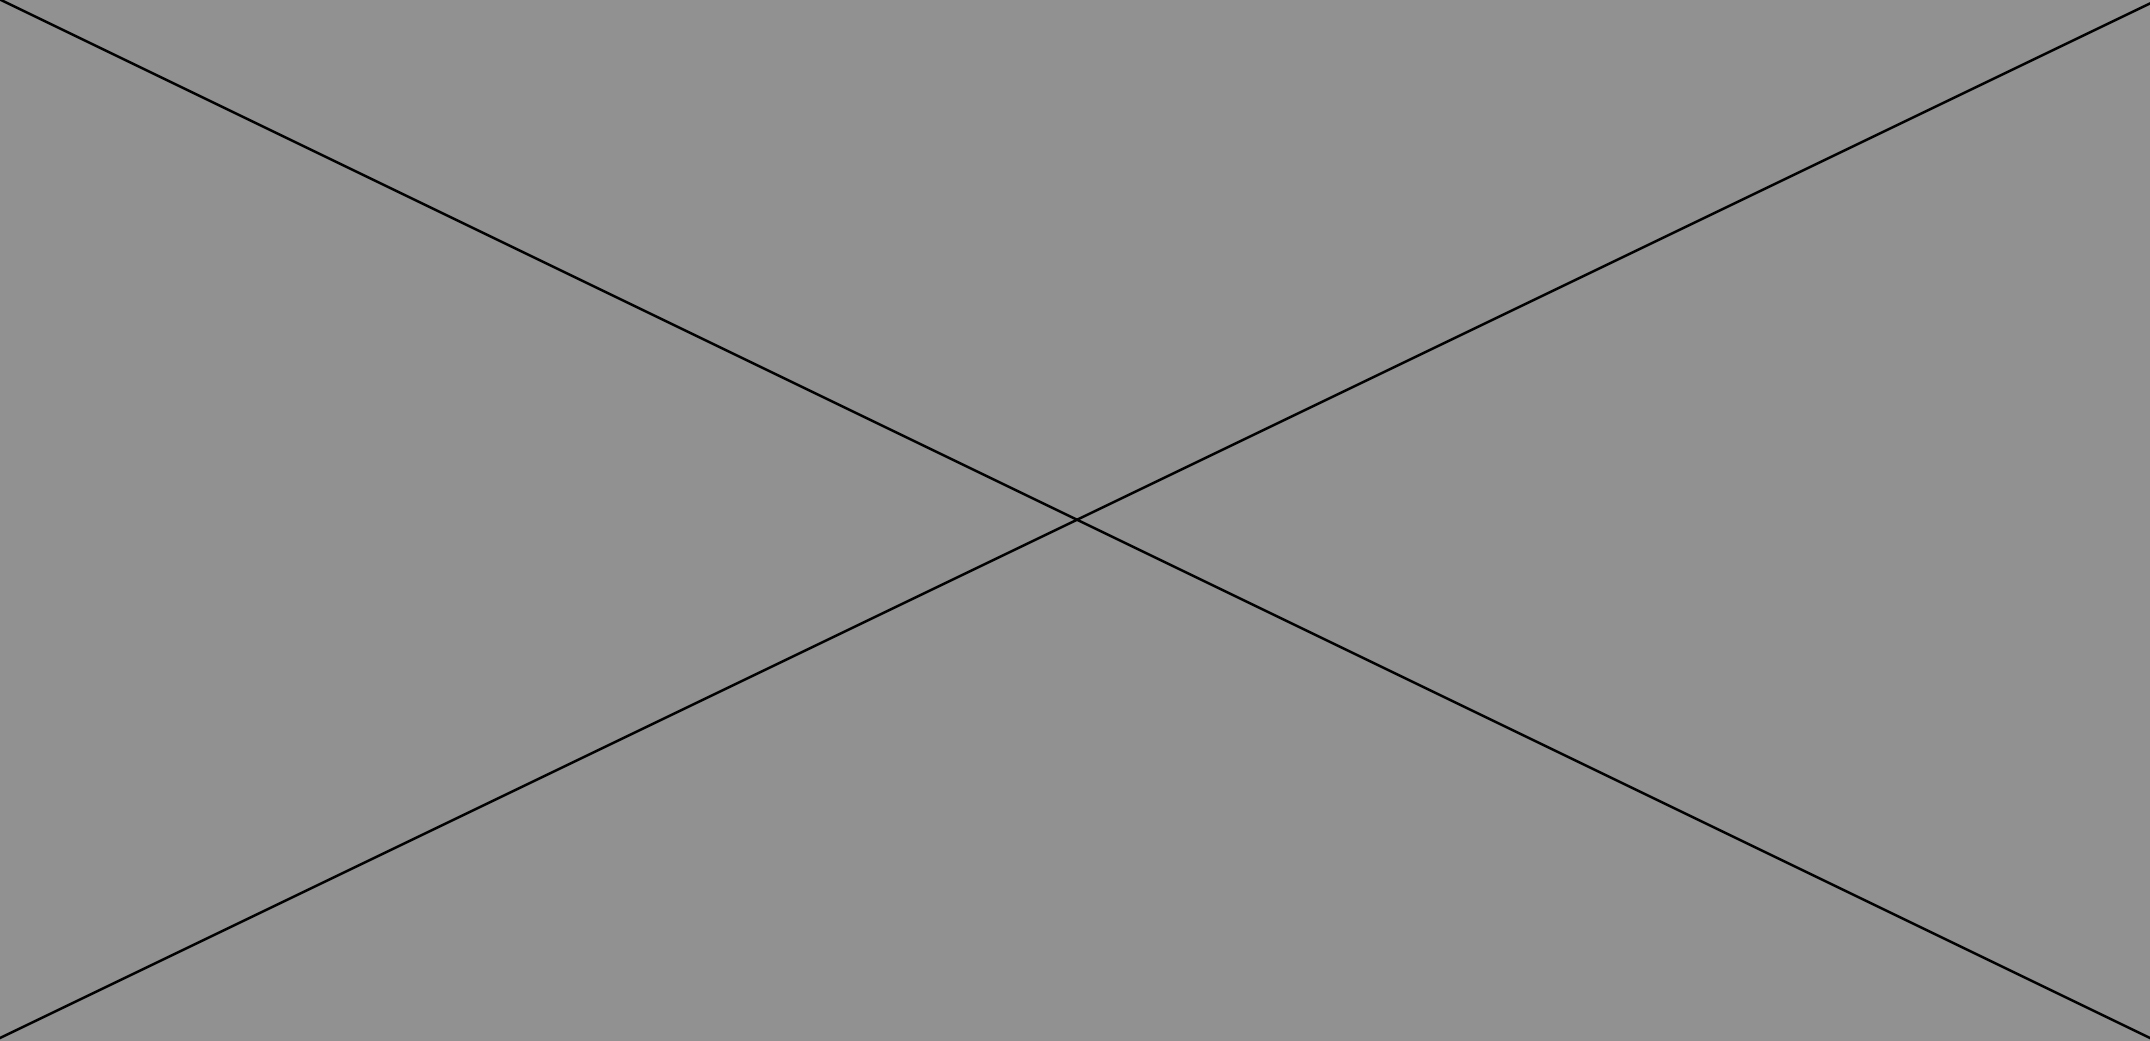
\includegraphics[width=.5\textwidth]{figures/placeholderImg.jpg}
  \caption[P3\_T3 Eye positioning]{P3\_T3 Eye positioning}
  \label{fig:P3_T3_pos}
\end{figure}

The two repetitions performed by P3 (Fig.~\ref{fig:P3_T3_pos})  show a gaze pattern which is pretty close to the expected one, with apparent good accuracy. An artifact is present during the ramp of the first repetition, and it could be a blink. While a large saccade performed after the ramp of the second repetition seems more an overshooting of the target.

\begin{figure}[h]
  \centering
  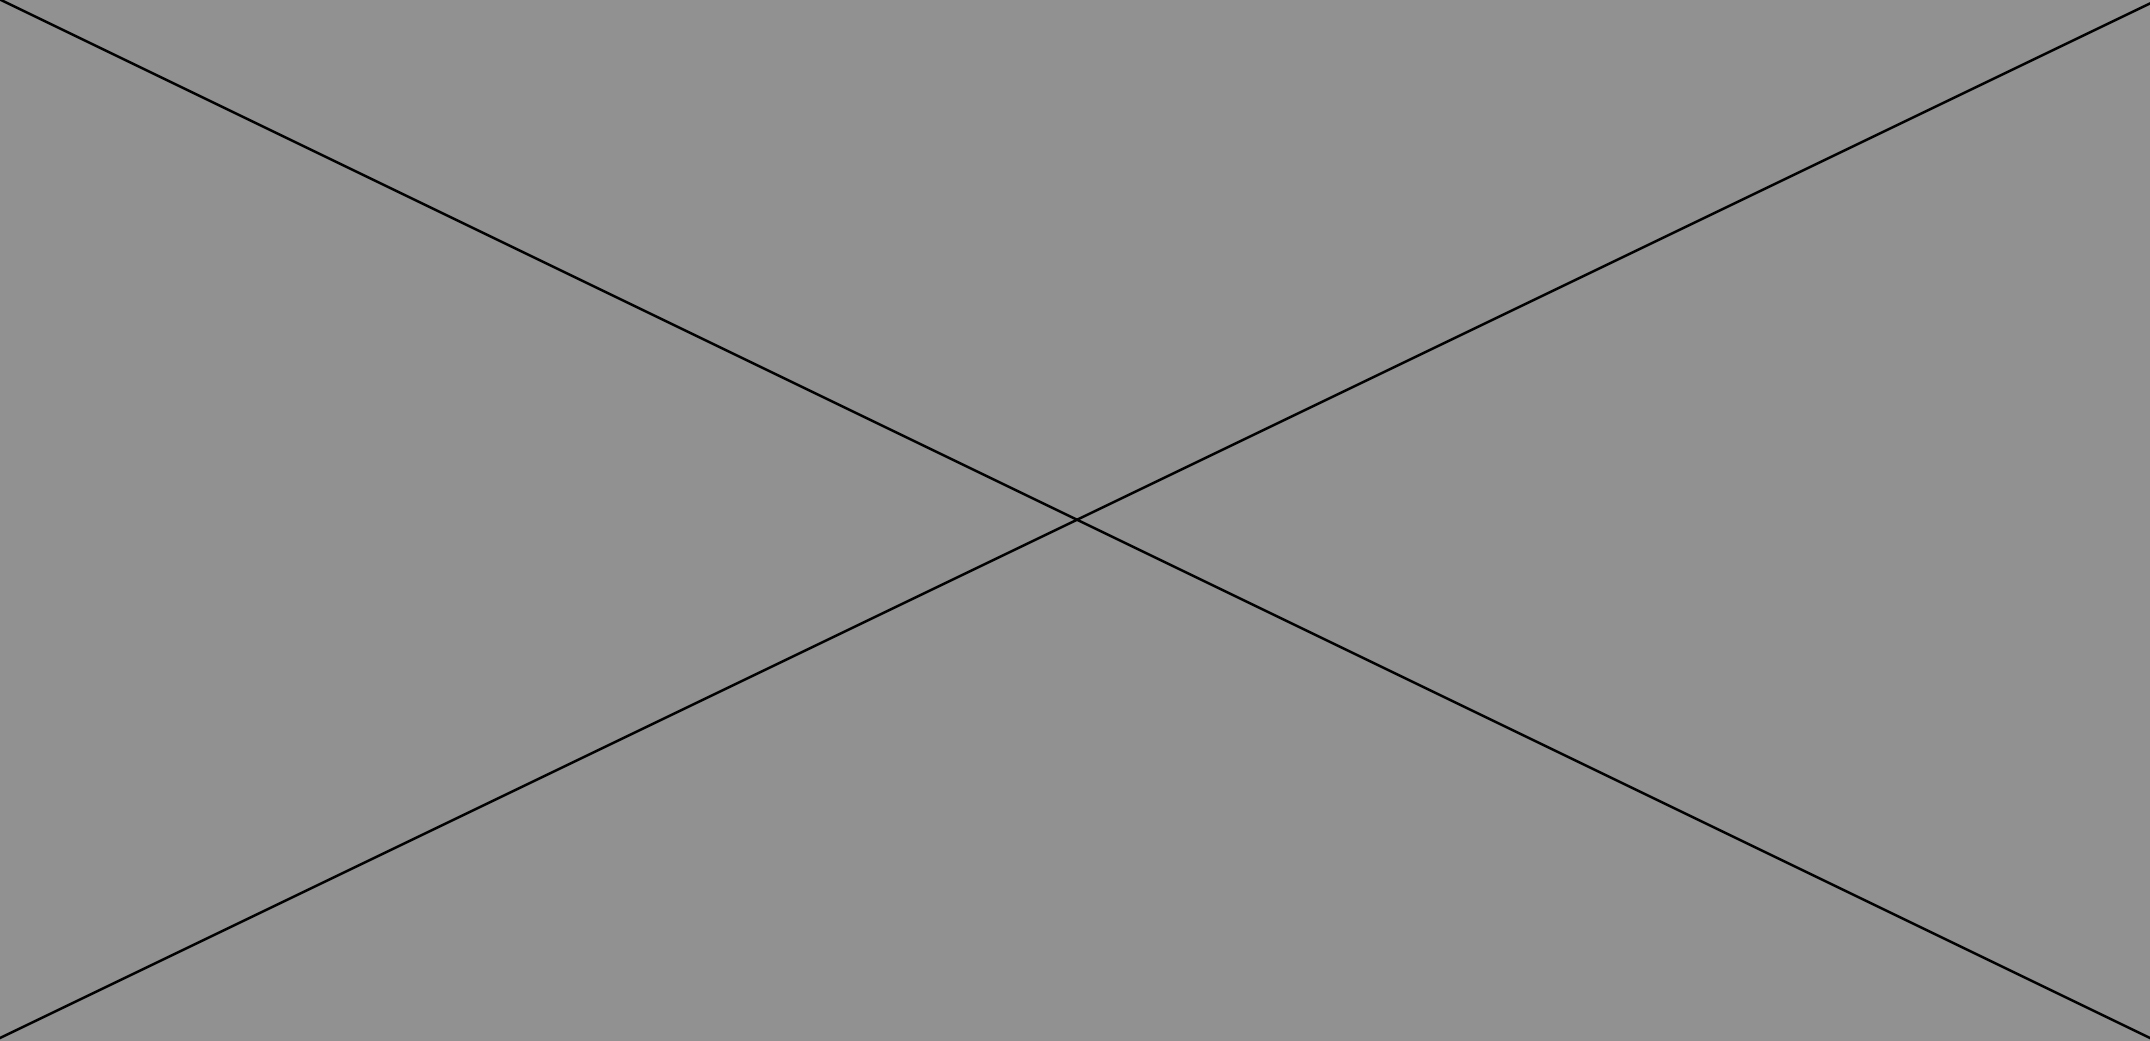
\includegraphics[width=.5\textwidth]{figures/placeholderImg.jpg}
  \caption[P3\_T3 pupil velocity]{P3\_T3 Pupil diameter and eye velocity}
  \label{fig:P3_T3_vel}
\end{figure}

Fig.~\ref{fig:P3_T3_vel} reveals how the velocity profile of the smooth pursuit ramp of the first repetition is overall flat, if not considering the artifact in between the pursuit, indicating smooth tracking. On the other hand, the series of peaks of eye velocity during the second ramp suggest more of a staircase pattern, with saccades and fixations in sequence rather a single smooth pursuit.

\subsection{P{1,2,3}\_T4 : Visually guided saccades visual stimuli}
\label{sec:P123_T4}


\subsubsection{P1\_T4}
\label{sec:P1_T1}

\begin{figure}[h]
  \centering
  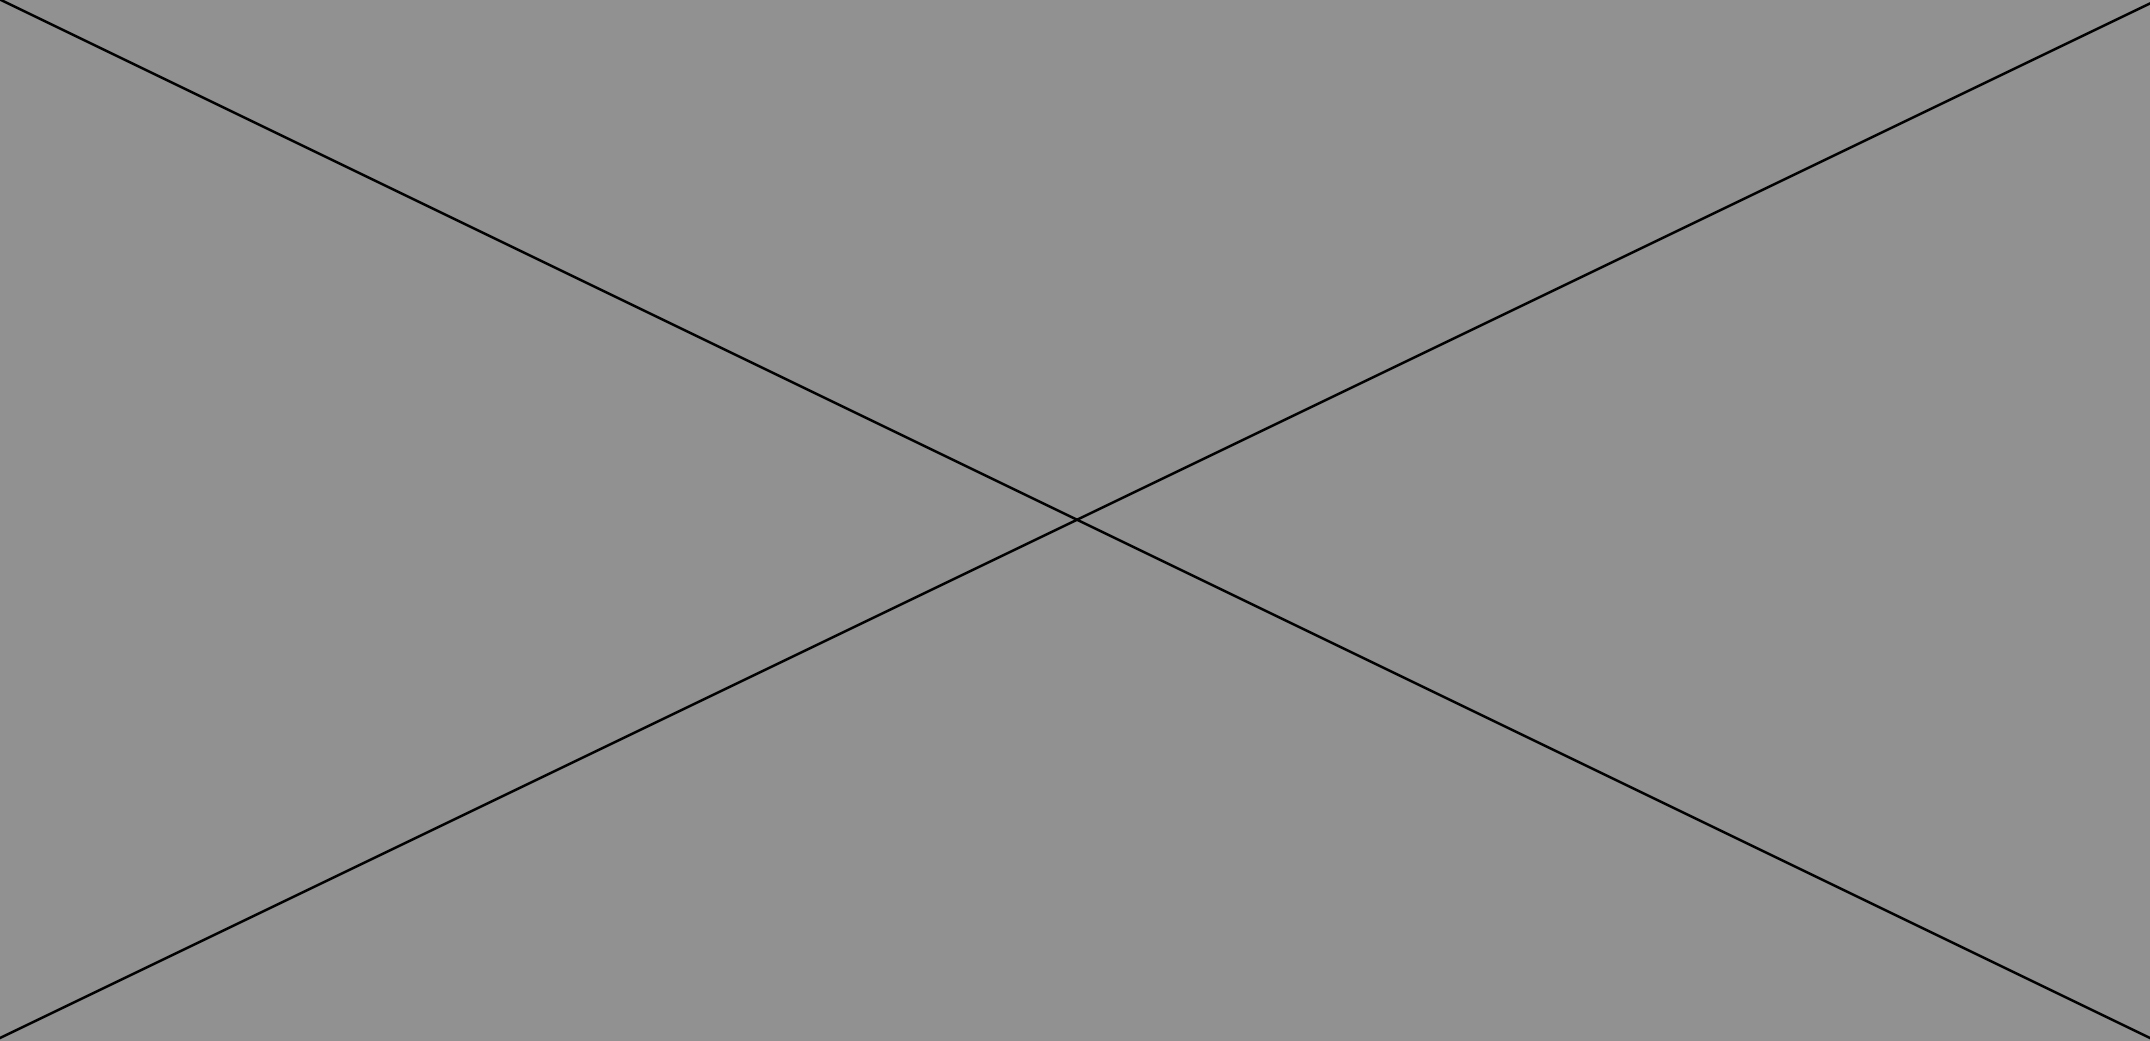
\includegraphics[width=.5\textwidth]{figures/placeholderImg.jpg}
  \caption[P1\_T4 Eye positioning]{P1\_T4 Eye positioning}
  \label{fig:P1_T4_pos}
\end{figure}

Fig.~\ref{fig:P1_T4_pos} show that the stimuli elicited the expected gaze pattern. A series of fixation on different points in the space is disrupted by quick eye movements, which are saccades. The fixation stabilization seems less precise from the pilot test reference dataset, and this could be due to small movement of the baby during the trial, or that the gaze stabilization improves further later in the children’s development. Some large artifacts are visible during fixations, and they probably are blinks, since they do not happen when the target moves from the center to the periphery or back.
The trial should have lasted for 43.7 s, but it has been stopped at 34.61 s since the child was evidently tired and not paying attention to the stimuli anymore. The chart shows the first 30 s, however no more evident gaze patterns are shown after 16 s.

\begin{figure}[h]
  \centering
  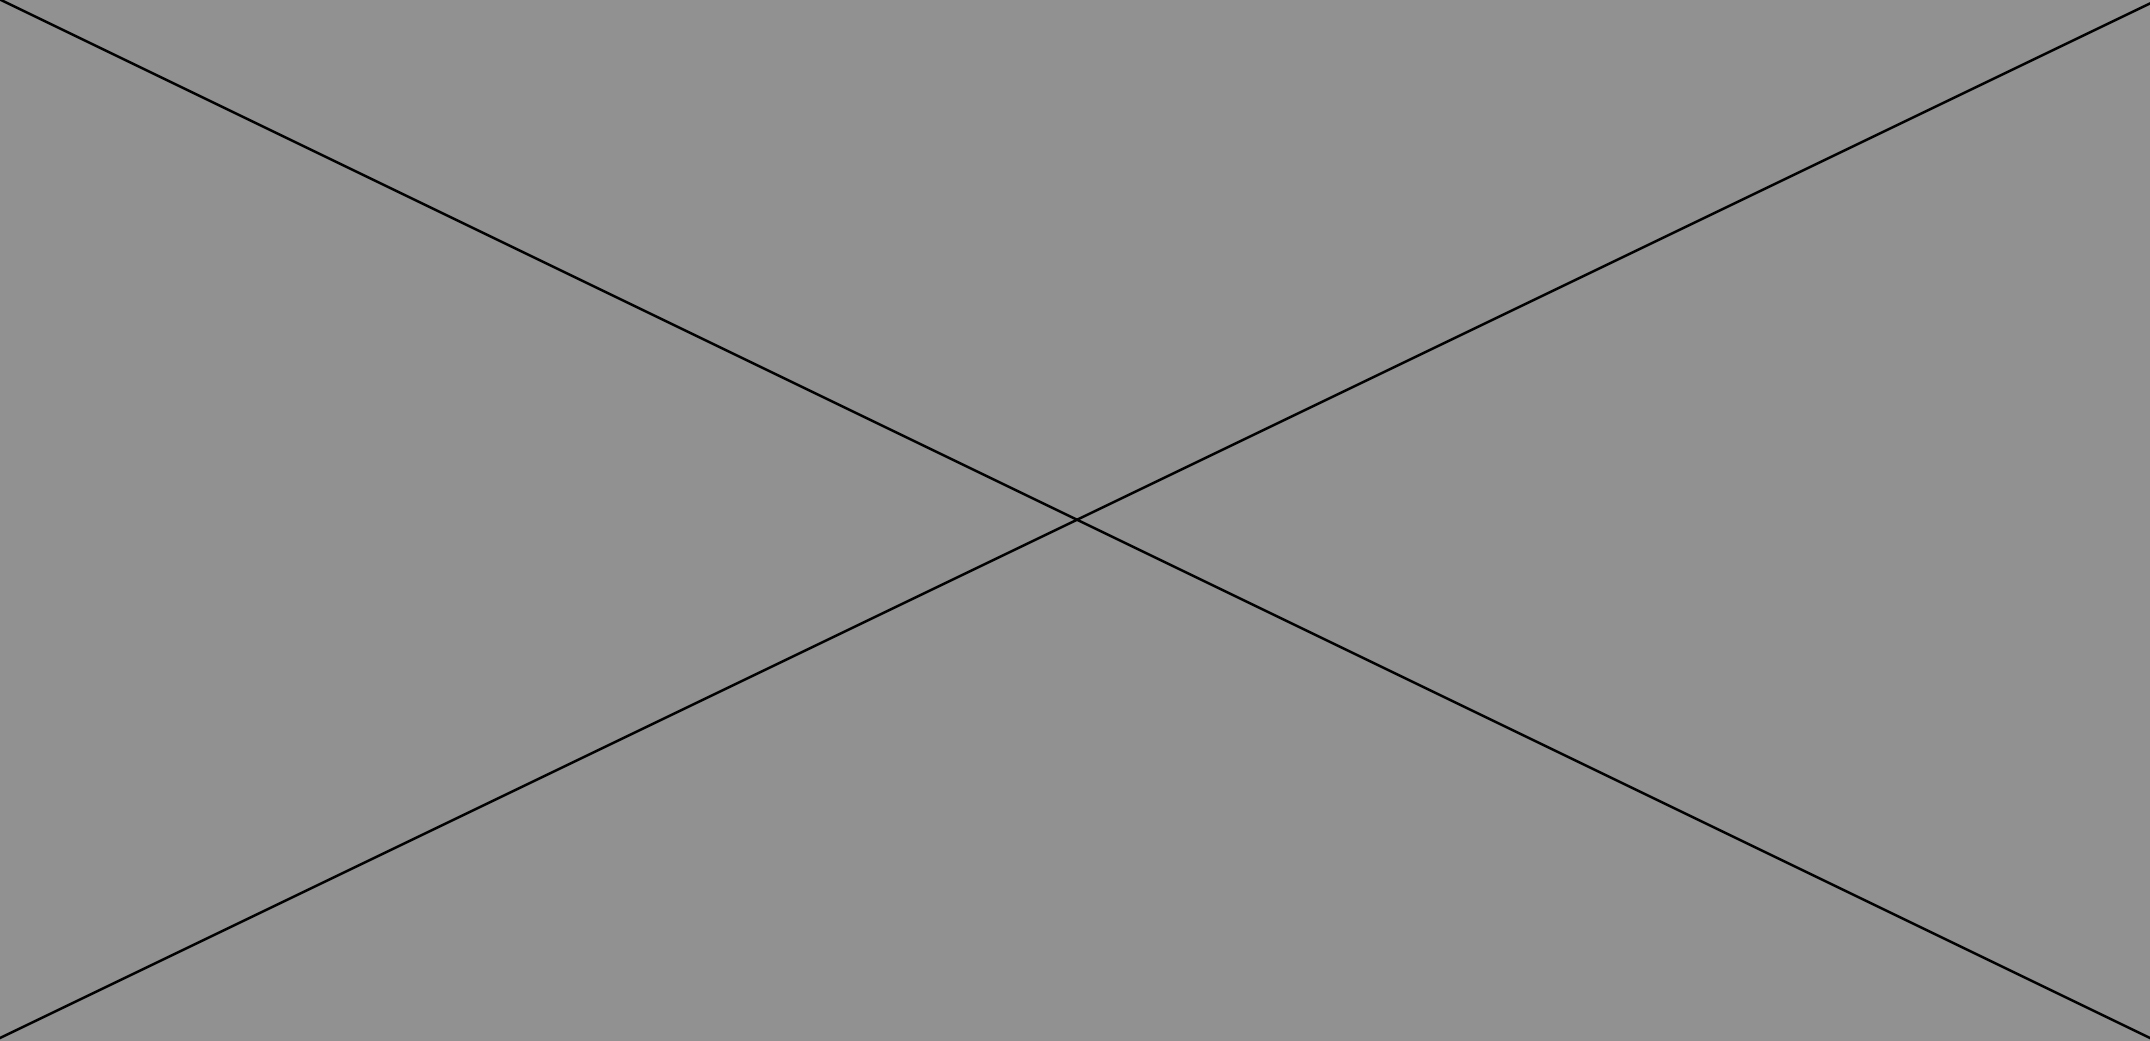
\includegraphics[width=.5\textwidth]{figures/placeholderImg.jpg}
  \caption[P1\_T4 pupil velocity]{P1\_T4 Pupil diameter and eye velocity}
  \label{fig:P1_T4_vel}
\end{figure}

Fig.~\ref{fig:P1_T4_vel} shows a series of consistent saccades, varying in peaks of velocity according to the amplitude of the saccade required, and in-between flatter velocity profiles of fixations, which however show constant low velocity small movements. Higher peaks in eye velocity are related to artifacts in the record, probably blinks. After 16 s the record seems to be too unreliable for being analyzed.

P2 and P3 did not perform Trial 4 (the visually guided saccades stimuli), and also P1 attended it for around one third of the time according to the tracking ratio. It seems that the experiment lasted for too long at this point, and the children’s attention faded in between the third stimulus and the third interstimulus material presentations. This made difficult to record data on Trial 4.

\subsection{Experiment notes}
\label{sec:expnotes}

Along with the eye tracker recordings, the researcher took some written notes during the experiments.

After finding a suitable spot in the home environment, P1’s calibration routines worked surprisingly good. They were fast and accurate, and the child did not need particular prompting for following the target with her gaze.
P2, during the experiment, was not particularly attracted by the first calibration procedure, which prevented to move on to the subsequent stimuli. Her mother then asked the researchers if she could help in directing P2’s attention toward the screen. The researchers welcomed the proposal, and the mother started to tell the children sentences like “what there is on the screen?” or “look at the screen”, and she pointed with her finger to the target. The mother performed this active reinforcement throughout all the experiment, and allowed to recover the child’s focus. The reinforcement was particularly useful during the calibration phases, which became shorter due to the child’s precise gaze directioning.

When a stimuli disappeared, the child often said “det er borte!” (“it disappeared!”, in English). She seemed surprised from the abrupt change between stimuli and interstimulus materials, especially in terms of the target picture. It is possible that she was expecting to see the same target performing different actions throughout the experiment stimuli. However, not meeting the child expectations fully can be a good way to keep his/her interest.\\
P2’s mother described that the child usually does not watch much television in general.

P3, the youngest participant, seemed particularly pleased with both the stimuli and the interstimulus materials. She giggled briefly when she saw the stimuli for the first time. She seemed very curious about the researchers’ presence, which made her turn frequently towards them and not following the stimuli materials on the screen. However, this reaction was expected. She was also younger than the target group, therefore the whole procedure was not completely tailored around children of her age group.
\chapter{Discussion}
\label{chap:discussion}

\chapter{Conclusion and suggestions for further research}
\label{chap:conclusion}

The developed eye tracking framework and procedure seems to elicit the expected gaze patterns in children between 12 and 24 months of age. Currently, no computational analysis on the raw data has been performed due to the researcher’s lack of domain knowledge. The next step in this research would be to contact and team up with mathematicians and software engineers, in order to refine and complete the framework in its data analysis part. As already described in \todo{section 3.5. Data analysis}, the studies from  \cite{giordano2017eyetrackersystem,jansson2013smoothpursuit,larsson2015detection} already push the research forward in this direction, showing the interest of the software engineering community for the data analysis of complex eye movements.

If in the future it will be possible to compute precisely the eye parameters of interest from the eye tracking recordings, then it will be possible to collect data from broader samples of children in the target age. This would allow to assess systematically the construct and content validity of oculomotor performance as early ASD indicator.

If some of the parameters tested by the framework would reveal to systematically predict ASD diagnosis, a common point of developmental divergence could be found within the wide variety of symptoms and conditions of ASD. Then, investigating further the neurological basis of the oculomotor impairment comparing also the results with neuroimaging studies, would be then the natural next step for the research. It would provide a clearer picture of what are the fundamental neurological pathways involved in ASD and possibly develop treatment to overcome the divergent development. 

Contextually to the search for adequate algorithms for the analysis of the recorded eye movements, the experimental procedure needs to be refined and improved. Finding a good balance between number of repetitions necessary for having reliable results, and length of the procedure will be a priority key point to fix. Shortening and refining both stimuli and interstimulus materials is the first step.The procedure seems to elicit and measure correct gaze patterns also for children younger than the target group. However, even further refinement of the procedure is needed if it should be applied it to younger children, given their shorter attention span and the difficulty to sit still for long times

While doing more experiments on larger samples, it is also possible that less eye parameters than the ones currently implemented the framework will reveal to be more sensitive. It is also possible that multiple paradigms provide similar results and become redundant. Therefore, the number of stimuli could decrease in future developments of the framework, shortening the time needed for the whole eye tracking session and at the same time leaving more space for the most reliable paradigms.

Finding and teaming up with clinical teams and structures to conduct experiments is vital for the development of the current research. The input of these professionals will be fundamental to define and perform possible longitudinal experimental designs. These could provide insights on the children’s developmental trajectories and the sensitiveness of the eye tracking methodology over the time.
Sharing and discussing the eye tracking measurements with these experts is also of extreme importance, either them being neuropsychiatrists, logopedist, etc. Eye movement patterns could be related to behavioral manifestations apparently distant as domain.

There are a number of features in the experiment procedure and stimuli which probably need to be researched in spin-off studies and then integrated in the general framework. Indeed, the framework should act as a catalyst for further research on each micro-experimental variable.\\
The velocity of the targets should be the priority parameter to fix, since it allows to calculate the gain of the eye movement, which in literature seems to be a key divergent parameter characterizing ASDg and therefore it needs to be measured accurately.\\
Another example could be that the color of the targets in the developed stimuli is currently arbitrary. \cite{franklin2008colorASD} report less accurate color perception in children with ASD of around 11 years of age, but not when it comes to discern category of colors. If the visual variable color could impact on attention or oculomotor performance is not known at the moment. This and other micro-variables might influence the outcomes of the measurement.

The experimental stimuli have been developed to be replicable and modifiable enough to be used also in different types of eye tracking research, perhaps on subjects with other neurodevelopmental disorders as well as TDg. It is conceivable that even if the stimuli will be used for other purposes, but on children belonging to the target age group, the insights coming from other studies could help to improve the stimuli parameters for this research as well.

In conclusion, there is still a long way to go before the framework will be functional to early ASD diagnosis, both in terms of refining the procedure and harmonizing it with the current clinical practice. Literature shows noticeable interest in the subject and eye tracking is a sensible tool for investigating divergent neurodevelopmental disorders. Interaction designers can keep on contributing to the scientific debate acting as mediators, facilitators and possibly leaders within this complex multidisciplinary research field. The ultimate goal of preventing small children to develop lifelong impairments provides enough motivation itself. The key point is to make more objective and precise instruments available to clinicians, both from pragmatic and economical points of view.


\ifthenelse{\boolean{HarvardCitations}}{%
	\bibliographystyle{agsm} % used for Harvard style references. Names - Humanities & Interaction Design
}{%
	\bibliographystyle{ntnuthesis/ntnuthesis} % used for Vancover style references. Numbers - Computer Science & Physics
}

\bibliography{master_thesis_bibliography}

\appendix
\chapter{Informed consent form [Norsk]}
\label{app:consentformNorsk}
The following appendix includes the informed consent form for the study in Norwegian language.



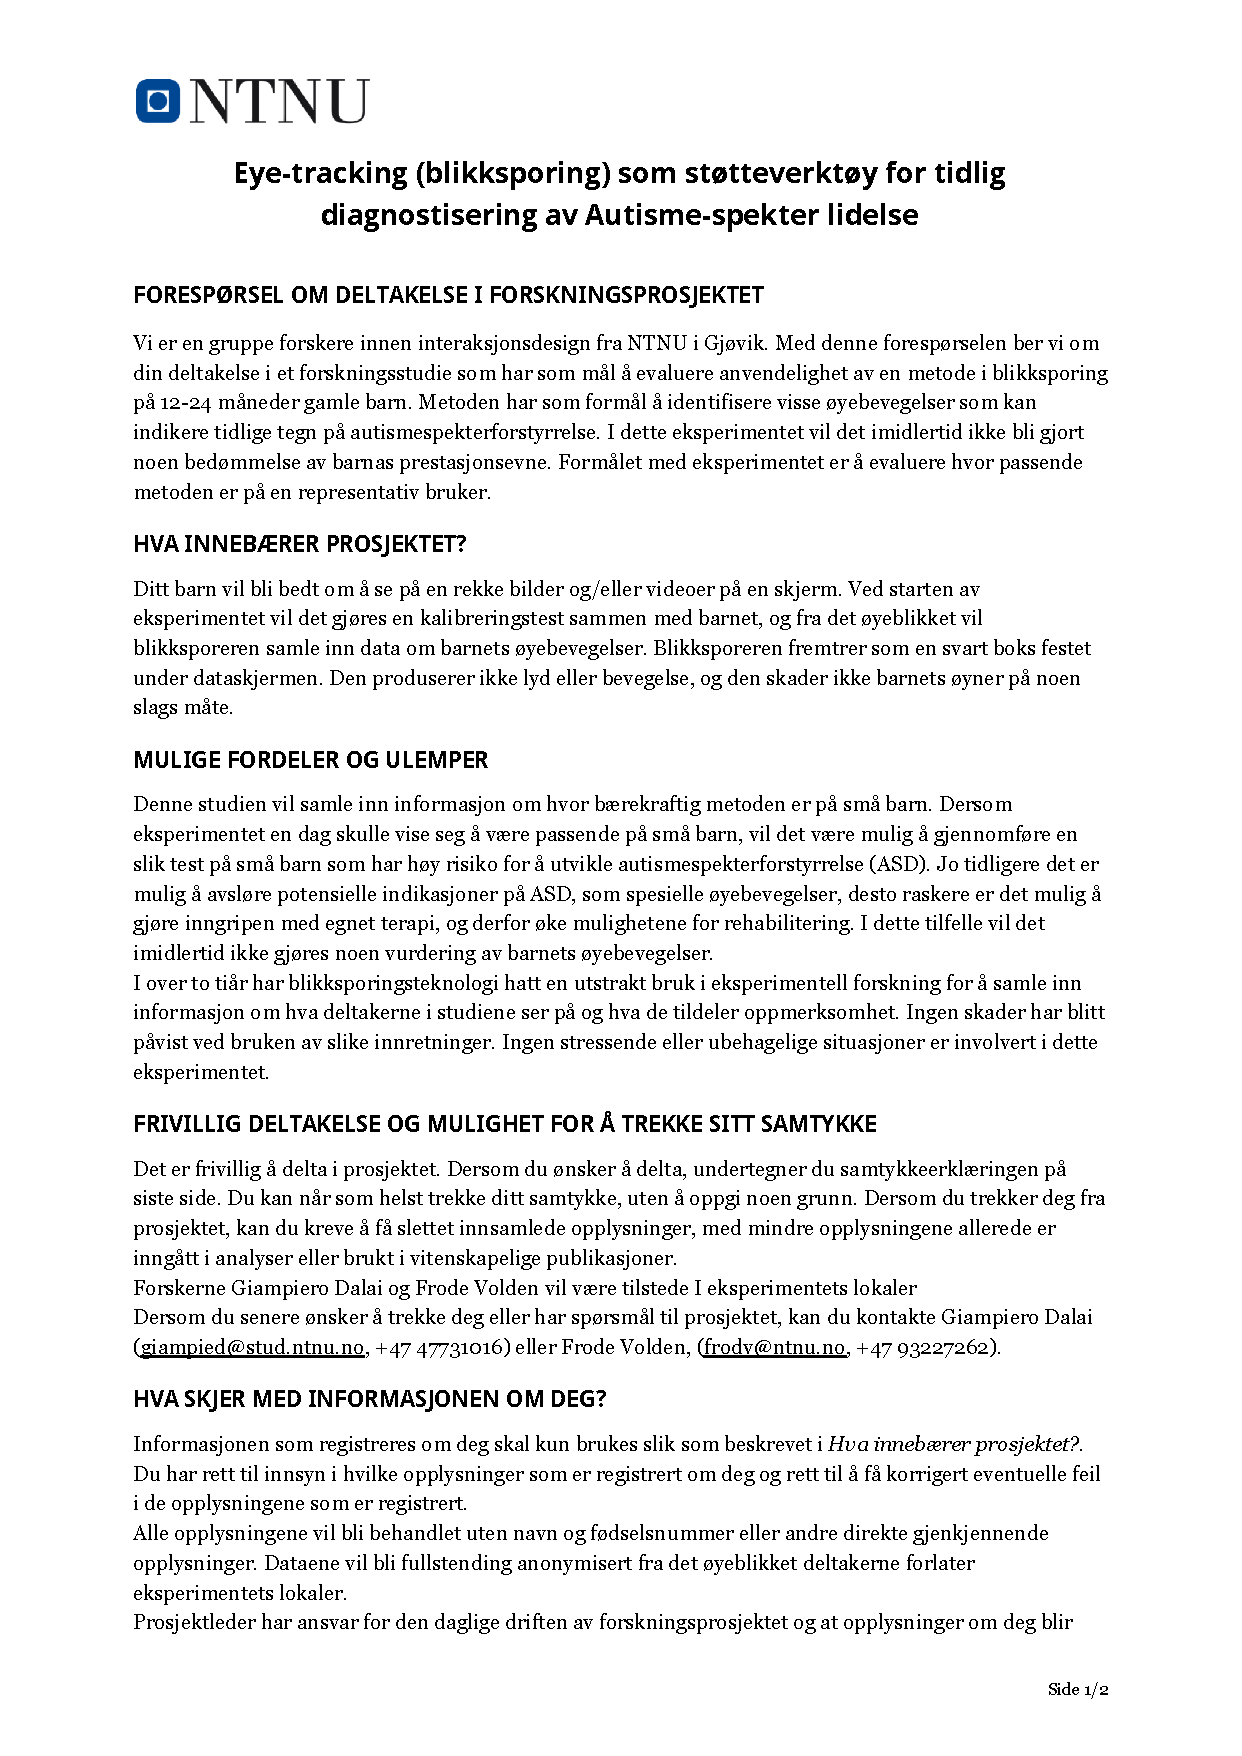
\includepdf[scale=1,pages={-}]{appendices/InformedConsentFormNorsk.pdf}
\chapter{Informed consent form [English]}
\label{app:consentformEnglish}
The following appendix includes the informed consent form for the study in English language.


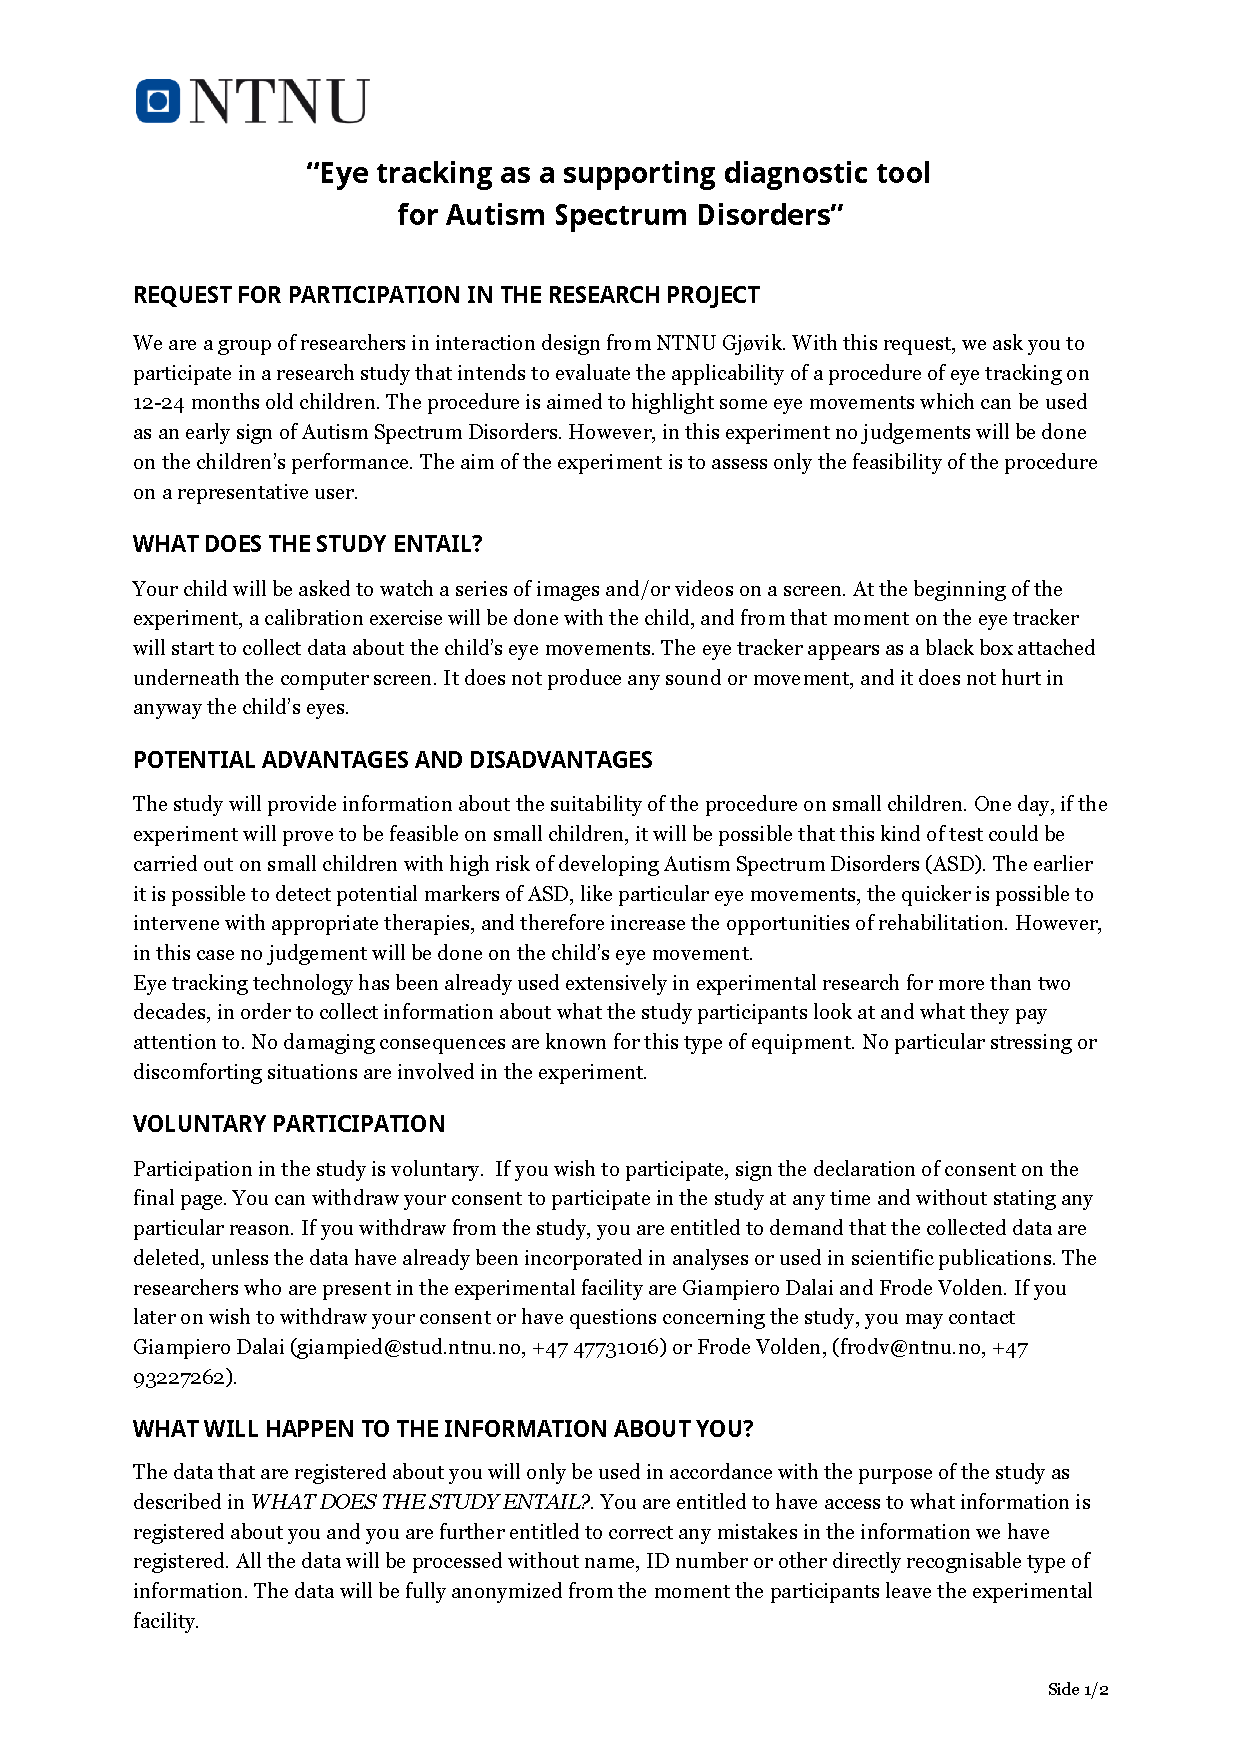
\includepdf[scale=1,pages={-}]{appendices/InformedConsentFormEnglish.pdf}
\chapter{Research protocol, detailed}
\label{app:researchprotocol}
The following appendix includes the detailed research protocol for the study.

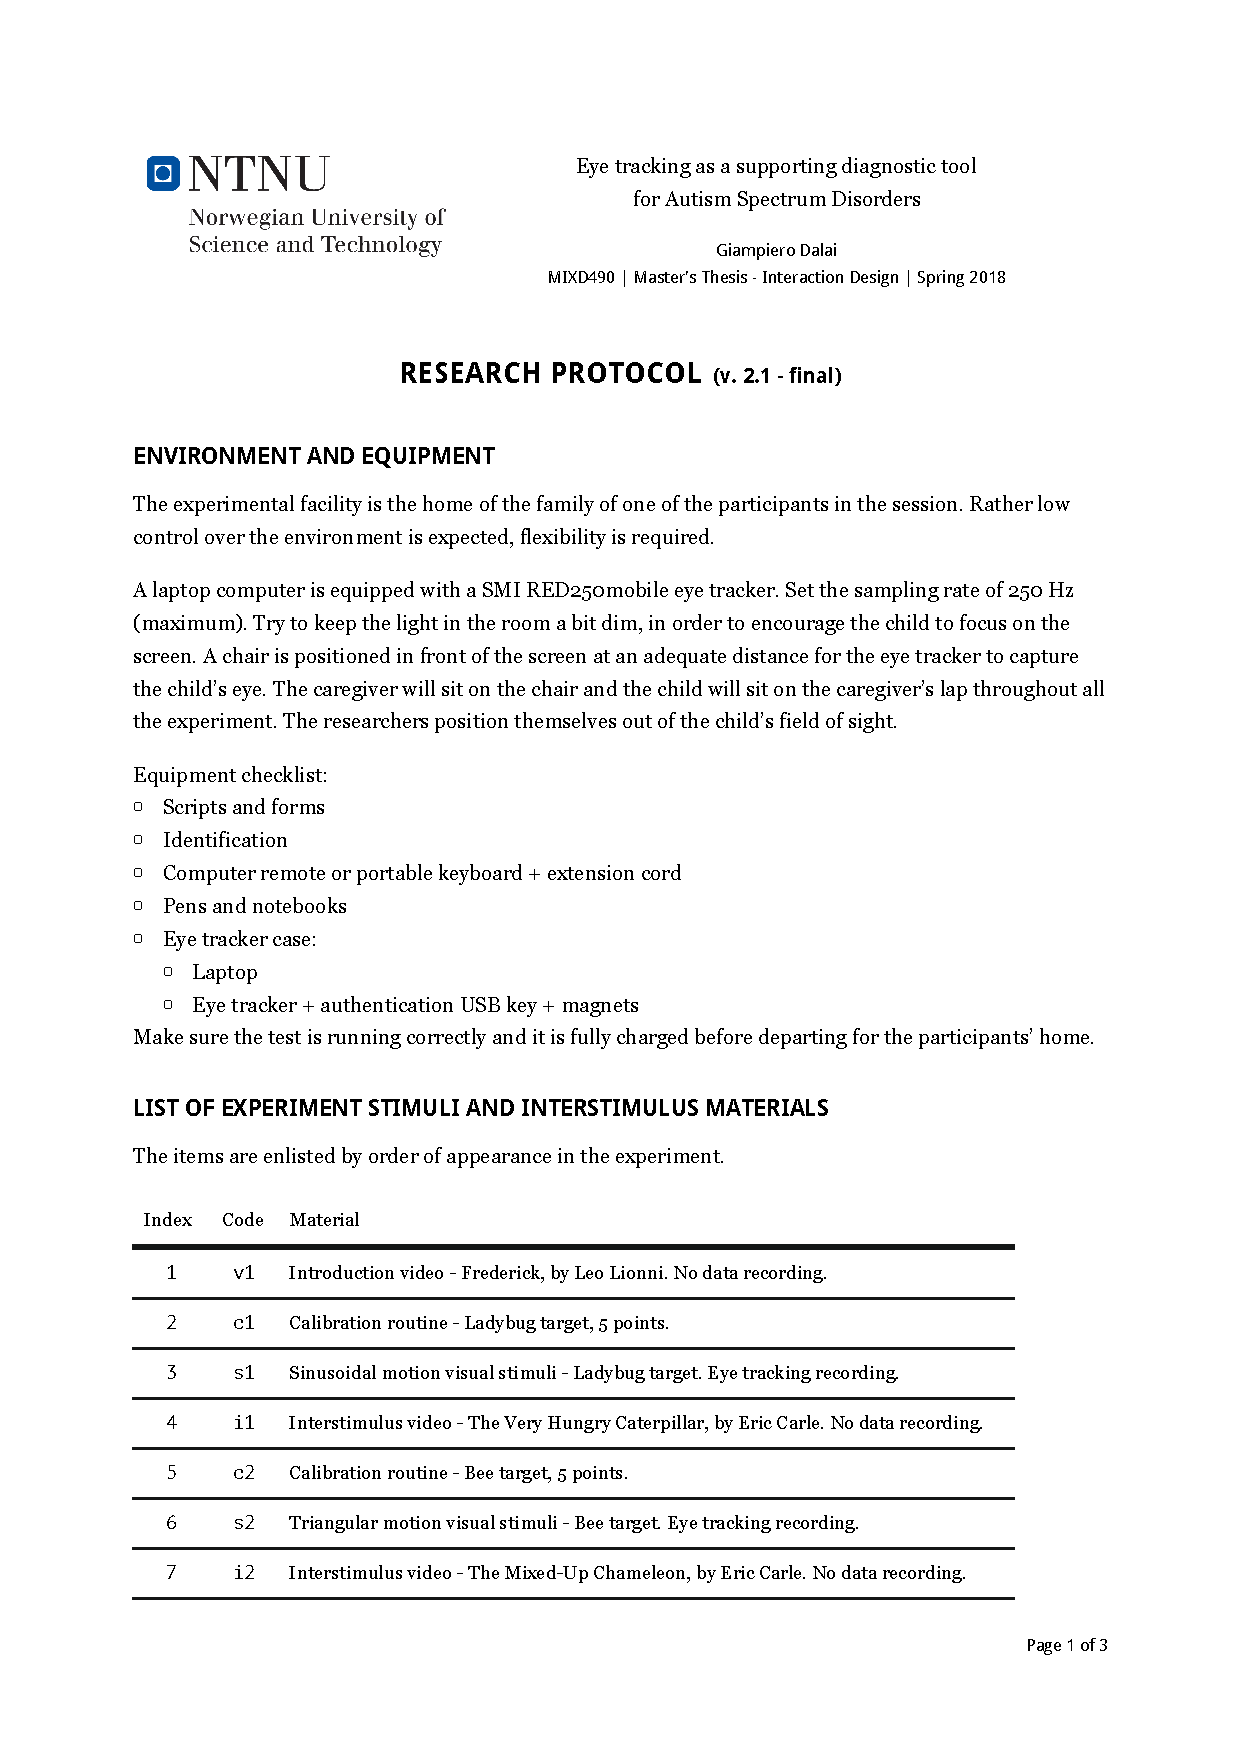
\includepdf[scale=1,pages={-}]{appendices/researchProtocol.pdf}
\chapter{Experiment stimuli detailed descriptions}
\label{app:stimulidescription}
The following appendix includes the detailed description of the visual stimuli used in the study. These data are generated by Processing 3 codes during the compilation of the executive files, which render the visual stimuli.

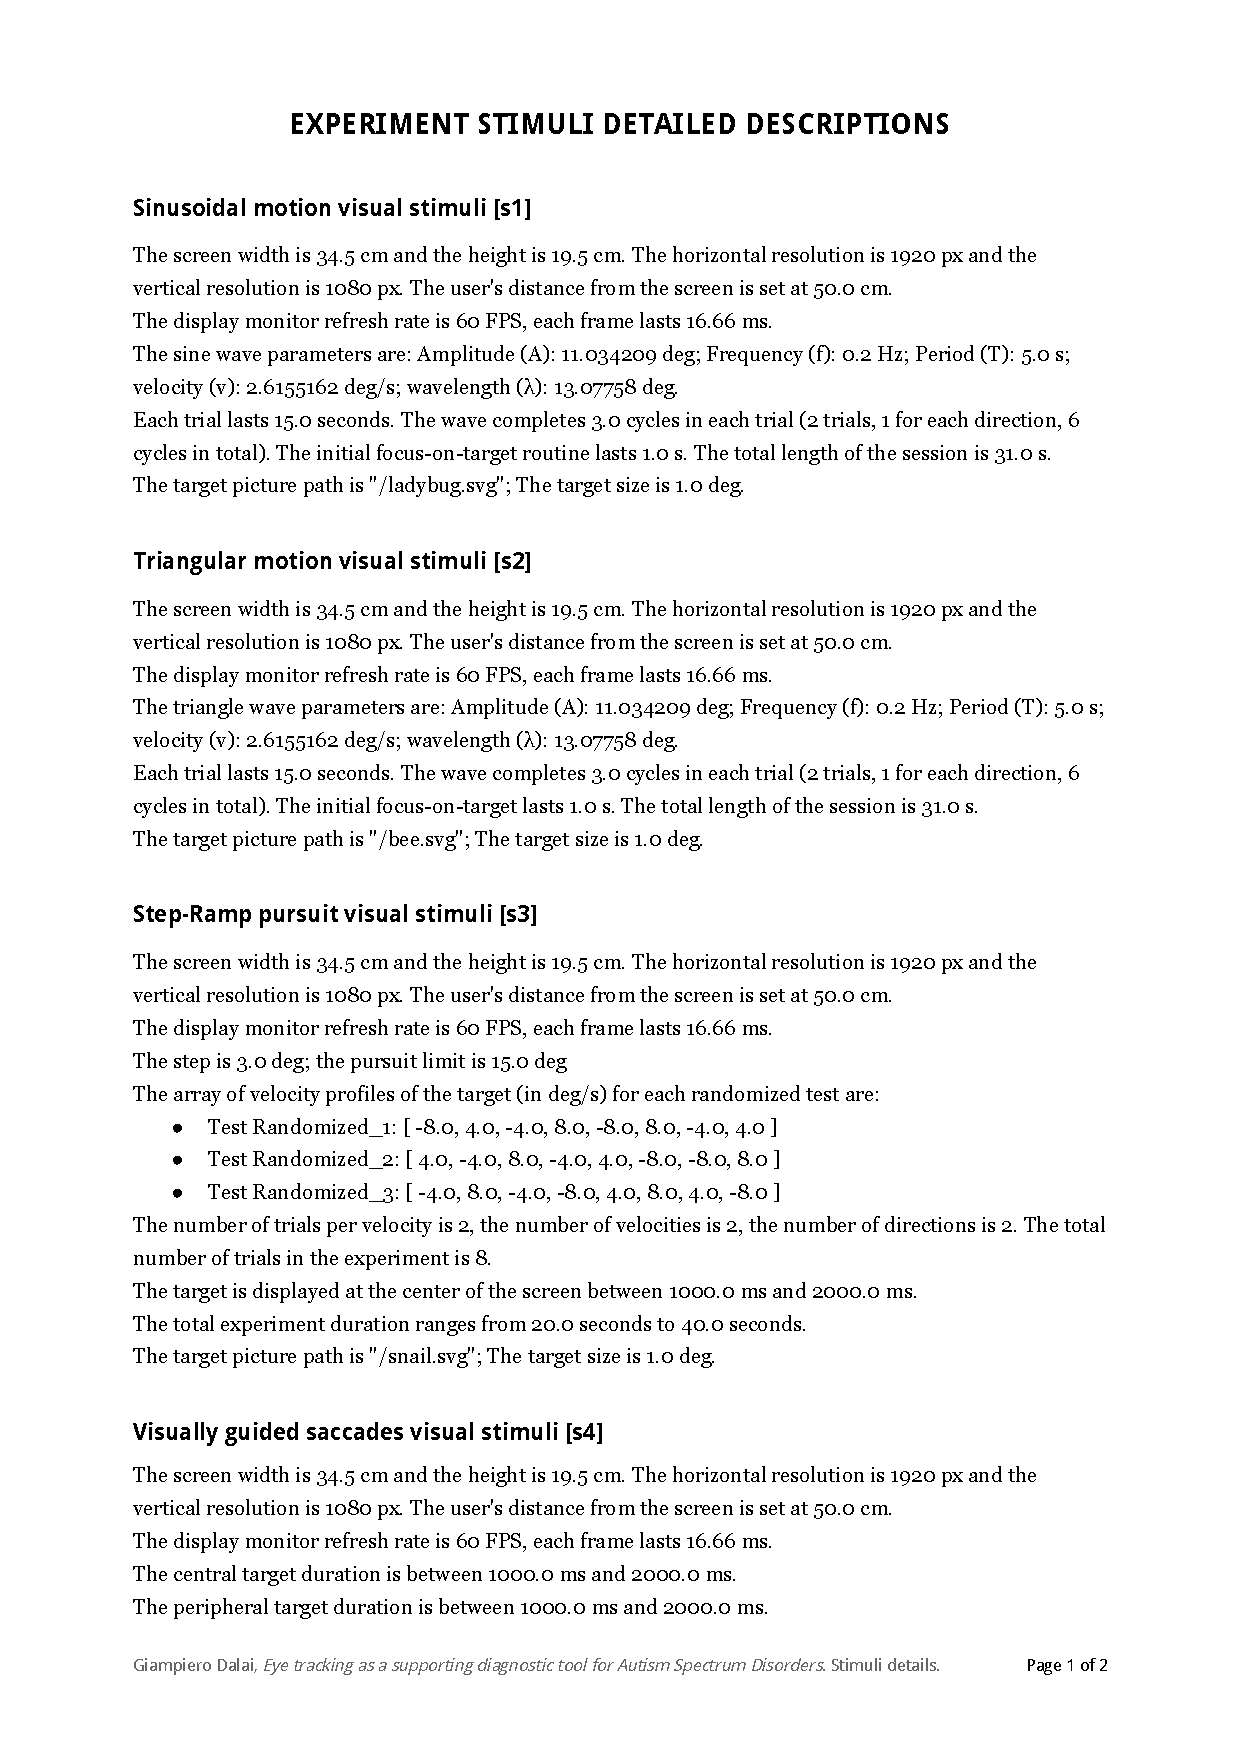
\includepdf[scale=1,pages={-}]{appendices/stimuliDescriptions.pdf}

\end{document}
